\documentclass[a4paper, onecolumn, 12pt]{IEEEtran}
%\documentclass[draftcls, onecolumn, a4paper, twoside]{IEEEtran}


% These values get used many times, so it is easier to define then once here.
% Module code
\def\modulecode{EPR 320 Electrical/Electronic/Computer Engineering Design}
% Assessment title
\def\assessment{Exam assignment}
%Project title
\def\ProjectTitle{Project Title}
% Group number
\def\groupnumber{45}
% Student details:
% Details of the first student
\def\firststudentname{Byron Norval}
\def\firststudentnumber{u21444758}
\def\firststudentcontribution{33.3\%}
% Details of the second student
\def\secondstudentname{Kyle Green}
\def\secondstudentnumber{u21441325}
\def\secondstudentcontribution{33.3\%}
% Details of the third student
\def\thirdstudentname{Francois Venter}
\def\thirdstudentnumber{U21471305}
\def\thirdstudentcontribution{33.3\%}


% Allows multi-line equations to be split over a number of pages.
\interdisplaylinepenalty=2500 


\usepackage{amsmath}
\usepackage{amssymb}
\usepackage{cite}
\usepackage{graphicx}
\usepackage{lastpage}
\usepackage{listings}
% \usepackage{minted}
% \renewcommand\theFancyVerbLine{\normalsize\arabic{FancyVerbLine}}
\usepackage{multirow}
\usepackage{paralist}
\usepackage{placeins}  % For \FloatBarrier
\usepackage{float}     % For [H] table/figure placement
%\usepackage{rotfloat}
%\usepackage{rotating}  % Package not available - commented out
\usepackage[tight,small]{subfigure}  % normalsize small footnotesize
\usepackage{tabularx}
\usepackage{tabulary}
\usepackage{booktabs}  % Professional quality tables
\usepackage{circuitikz} % For circuit diagrams

% I prefer this to the default font.
\usepackage{newtxmath}
\usepackage{newtxtext}
\renewcommand{\rmdefault}{ntxtlf} 
%https://tex.stackexchange.com/questions/347566/math-digits-are-rendered-in-cm-when-using-libertine-and-newtxmath-with-xelatex-i


% Set the page format up.
\usepackage{geometry}
\geometry{includefoot}
\geometry{paper=a4paper}
\geometry{left=25mm}
\geometry{right=25mm}
\geometry{top=25mm}
\geometry{bottom=20mm}
\geometry{headsep=10mm}
\geometry{footskip=10mm}
%\geometry{columnsep=4mm}


\usepackage[pdftex]{hyperref}
%\hypersetup{pdfborder={0 0 0.2}}
\usepackage{xcolor}
\definecolor{darkred}{rgb}{0.8,0,0}
\definecolor{darkgreen}{rgb}{0,0.45,0}
\definecolor{darkblue}{rgb}{0,0,0.3}

% Set the PDF properties of the document.
\hypersetup{%
  pdftitle={\modulecode-- \assessment},
  pdfauthor={Group \groupnumber}}


\usepackage{fancyhdr}
% Set the page format up.
\def\pagenumberfooter{\thepage}
\fancypagestyle{plain}{%
  \fancyhf{}
  \lhead{}
  \rhead{}
  \lfoot{}
%  \cfoot{Confidential}
  \rfoot{\thepage}
  \renewcommand{\headrulewidth}{0pt}
  \renewcommand{\footrulewidth}{0pt}
}
\def\pagenumberfooter{\thepage}
\fancypagestyle{fancy}{%
  %\fancyhf{}
  %\lhead{}
  %\rhead{}
  %\lfoot{\modulecode~-- \assessment~-- Group \groupnumber}
%  \cfoot{Confidential}
  \rfoot{\thepage}
  \renewcommand{\headrulewidth}{0pt}
  \renewcommand{\footrulewidth}{0.0pt}
}


\hyphenation{mono-pulse}
\hyphenation{retro-directive}


% I prefer this to the default versions - feel free to disagree.
%\usepackage[cal=boondoxo]{mathalfa}  % Package not available - commented out
\renewcommand{\Re}{\mathcal{R\hspace{-0.2em}e\hspace{-0.1em}}}
\renewcommand{\Im}{\mathcal{I\hspace{-0.25em}m\hspace{-0.15em}}}

\newlength{\equalswidth}
\settowidth{\equalswidth}{$ =~ $}
\newcommand{\eqsplitline}{\nonumber \\ & \hspace{\equalswidth}}
\newcommand{\eqsplitaligned}{\\ & \hspace{\equalswidth}}



%\def\today{27 March 2018}
% Get the Day Month Year format.
\def\today{%
  \number\day
  \space
  \ifcase\month\or January\or February\or March\or April\or May\or
  June\or July\or August\or September\or October\or November\or
  December\fi
  \space
  \number\year
}


% Allow large floats.
\renewcommand\topfraction{1}
\renewcommand\bottomfraction{0}
\renewcommand\textfraction{0}
\renewcommand\floatpagefraction{1}
\setcounter{topnumber}{10}
\setcounter{totalnumber}{10}


% Increase the figure caption font size.
\usepackage[font=normalsize]{caption}

% Deal with missing images which are not directly included in the repository
\newcommand{\noimage}{%
  \fbox{\parbox[t][0.3\textwidth][c]{0.48\textwidth}{\centering Image file is missing.}}
%  \setlength{\fboxsep}{-\fboxrule}%
%  \fbox{\phantom{\rule{10pt}{10pt}}File missing\phantom{\rule{10pt}{10pt}}}% Framed box
}
\let\includegraphicsoriginal\includegraphics
\renewcommand{\includegraphics}[2][width=\textwidth]
{%
  \IfFileExists{#2}
  {\includegraphicsoriginal[#1]{#2}}%
  {\noimage}%
%  {\fbox{\includegraphicsoriginal[#1]{drawings/gripen}\makebox[0pt]{File #2 is missing.}}}%
}

% Centred column in tabularx.
\newcolumntype{Y}{>{\centering\arraybackslash}X}

% Redefine section titles to be left-aligned and bold
\usepackage{titlesec}
\titleformat{\section}{\bfseries\Large}{\thesection}{1em}{}
\titleformat{\section}{\fontsize{18}{22}\bfseries\rmfamily}{\thesection}{1em}{}

\titleformat{\subsection}{\fontsize{16}{20}\bfseries\rmfamily}{\thesubsection}{1em}{}
\renewcommand{\thesubsection}{\thesection.\arabic{subsection}}

\titleformat{\subsubsection}{\fontsize{14}{18}\bfseries\rmfamily}{\thesubsubsection}{1em}{}
\renewcommand{\thesubsubsection}{\thesection.\arabic{subsection}.\arabic{subsubsection}}

% Format paragraph and subparagraph
\titleformat{\paragraph}{\fontsize{12}{15}\bfseries\rmfamily}{\theparagraph}{1em}{}
\titlespacing*{\paragraph}{0pt}{1em}{0.5em}

\titleformat{\subparagraph}{\fontsize{11}{14}\bfseries\rmfamily}{\thesubparagraph}{1em}{}
\titlespacing*{\subparagraph}{0pt}{0.8em}{0.4em}

% Define numbering for subsubsubsections as 2.5.1.1
\newcounter{subsubsubsection}[subsubsection]
\renewcommand{\thesubsubsubsection}{\thesubsubsection.\arabic{subsubsubsection}}

% Define the subsubsubsection command with a new line after heading
\titleformat{\subsubsubsection}{\fontsize{12}{15}\itshape}{\thesubsubsubsection}{1em}{} 

% Command for subsubsubsection
\newcommand{\subsubsubsection}[1]{%
    \refstepcounter{subsubsubsection}%
    \vspace{0.2em} % Adjusts space before
    \noindent\textit{\thesubsubsubsection\ #1}\par
    \vspace{-0.5em} % Adjusts space after
}


% Define numbering for subsubsubsubsections as 2.5.1.1.1
\newcounter{subsubsubsubsection}[subsubsubsection]
\renewcommand{\thesubsubsubsubsection}{\thesubsubsubsection.\arabic{subsubsubsubsection}}

% Command for subsubsubsubsection (11pt, italic, slightly smaller)
\newcommand{\subsubsubsubsection}[1]{%
    \refstepcounter{subsubsubsubsection}%
    \vspace{0.15em} % Adjusts space before
    \noindent{\fontsize{11}{14}\selectfont\itshape\thesubsubsubsubsection\ #1}\par
    \vspace{-0.5em} % Adjusts space after
}


% Define numbering for subsubsubsubsubsections as 2.5.1.1.1.1
\newcounter{subsubsubsubsubsection}[subsubsubsubsection]
\renewcommand{\thesubsubsubsubsubsection}{\thesubsubsubsubsection.\arabic{subsubsubsubsubsection}}

% Command for subsubsubsubsubsection (10pt, italic, smallest)
\newcommand{\subsubsubsubsubsection}[1]{%
    \refstepcounter{subsubsubsubsubsection}%
    \vspace{0.1em} % Adjusts space before
    \noindent{\fontsize{10}{13}\selectfont\itshape\thesubsubsubsubsubsection\ #1}\par
    \vspace{-0.5em} % Adjusts space after
}
\usepackage[acronym]{glossaries}
\makeglossaries
\setglossarystyle{long}
% Increase the gap between acronym and description
\setlength{\glsdescwidth}{0.8\textwidth}
\setlength{\glspagelistwidth}{0.15\textwidth}
% acronyms/acronyms.tex
% Define acronyms for automatic first-use expansion and list generation.

% ==================== PROJECT-SPECIFIC ACRONYMS ====================
\newacronym{marv}{MARV}{Miniature Autonomous Robotic Vehicle}
\newacronym{snc}{SNC}{State-and-Navigation Control}
\newacronym{ss}{SS}{Sensor Subsystem}
\newacronym{mdps}{MDPS}{Motor Drive and Power Subsystem}
\newacronym{scs}{SCS}{Structured Command Set}
\newacronym{navcon}{NAVCON}{Navigation Control}
\newacronym{hmi}{HMI}{Human-Machine Interface}
\newacronym{pec}{PEC}{Project Evaluation Criteria}
\newacronym{hub}{HUB}{Hardware Unit Bench (testing interface)}
\newacronym{eoc}{EoC}{End-of-Calibration}
\newacronym{eom}{EoM}{End-of-Maze}
\newacronym{sos}{SOS}{Save Our Ship (emergency state)}
\newacronym{ist}{IST}{Instruction Type}
\newacronym{spl}{SPL}{Sound Pressure Level}

% ==================== SYSTEMS ENGINEERING ====================
\newacronym{qtp}{QTP}{Qualification Test Procedure}
\newacronym{icd}{ICD}{Interface Control Document}
\newacronym{rtm}{RTM}{Requirements Traceability Matrix}
\newacronym{opscon}{OpsCon}{Operational Concept}
\newacronym{stp}{STP}{System Test Plan}
\newacronym{vv}{V\&V}{Verification and Validation}
\newacronym{fsm}{FSM}{Finite State Machine}
\newacronym{hil}{HIL}{Hardware-in-the-Loop}
\newacronym{mtbf}{MTBF}{Mean Time Between Failures}
\newacronym{mttr}{MTTR}{Mean Time To Repair}

% ==================== HARDWARE & MICROCONTROLLER ====================
\newacronym{mcu}{MCU}{Microcontroller Unit}
\newacronym{cpu}{CPU}{Central Processing Unit}
\newacronym{gpio}{GPIO}{General Purpose Input/Output}
\newacronym{adc}{ADC}{Analogue-to-Digital Converter}
\newacronym{dac}{DAC}{Digital-to-Analogue Converter}
\newacronym{pwm}{PWM}{Pulse Width Modulation}
\newacronym{led}{LED}{Light Emitting Diode}
\newacronym{pcb}{PCB}{Printed Circuit Board}
\newacronym{ic}{IC}{Integrated Circuit}
\newacronym{mosfet}{MOSFET}{Metal-Oxide-Semiconductor Field-Effect Transistor}
\newacronym{afe}{AFE}{Analogue Front-End}
\newacronym{isr}{ISR}{Interrupt Service Routine}

% ==================== COMMUNICATION PROTOCOLS ====================
\newacronym{uart}{UART}{Universal Asynchronous Receiver-Transmitter}
\newacronym{iic}{I\textsuperscript{2}C}{Inter-Integrated Circuit}
\newacronym{spi}{SPI}{Serial Peripheral Interface}
\newacronym{usb}{USB}{Universal Serial Bus}
\newacronym{rf}{RF}{Radio Frequency}

% ==================== NETWORKING & DATA ====================
\newacronym{wifi}{Wi-Fi}{Wireless Fidelity}
\newacronym{http}{HTTP}{Hypertext Transfer Protocol}
\newacronym{rest}{REST}{Representational State Transfer}
\newacronym{api}{API}{Application Programming Interface}
\newacronym{json}{JSON}{JavaScript Object Notation}
\newacronym{csv}{CSV}{Comma-Separated Values}
\newacronym{ws}{WS}{WebSocket}

% ==================== DATA INTEGRITY & PROTOCOL ====================
\newacronym{crc}{CRC}{Cyclic Redundancy Check}
\newacronym{sof}{SOF}{Start of Frame}
\newacronym{eof}{EOF}{End of Frame}
\newacronym{ack}{ACK}{Acknowledge}
\newacronym{nak}{NAK}{Negative Acknowledge}
\newacronym{ber}{BER}{Bit Error Rate}

% ==================== MEMORY & STORAGE ====================
\newacronym{ram}{RAM}{Random Access Memory}
\newacronym{rom}{ROM}{Read-Only Memory}
\newacronym{eeprom}{EEPROM}{Electrically Erasable Programmable Read-Only Memory}
\newacronym{rtc}{RTC}{Real-Time Clock}
\newacronym{dma}{DMA}{Direct Memory Access}

% ==================== CONTROL & SIGNAL PROCESSING ====================
\newacronym{pid}{PID}{Proportional-Integral-Derivative}
\newacronym{dsp}{DSP}{Digital Signal Processing}

% ==================== ELECTROMAGNETIC & SAFETY ====================
\newacronym{emi}{EMI}{Electromagnetic Interference}
\newacronym{emc}{EMC}{Electromagnetic Compatibility}
\newacronym{dc}{DC}{Direct Current}

% ==================== DEVELOPMENT TOOLS ====================
\newacronym{ide}{IDE}{Integrated Development Environment}
\newacronym{cad}{CAD}{Computer-Aided Design}
\newacronym{git}{Git}{Distributed Version Control System}

% ==================== OTHER TECHNICAL TERMS ====================
\newacronym{fpga}{FPGA}{Field-Programmable Gate Array}
\newacronym{iot}{IoT}{Internet of Things}

% ==================== ESP32 & EMBEDDED SYSTEMS ====================
\newacronym{soc}{SoC}{System on Chip}
\newacronym{rtos}{RTOS}{Real-Time Operating System}
\newacronym{wdt}{WDT}{Watchdog Timer}
\newacronym{ota}{OTA}{Over-The-Air (firmware update)}
\newacronym{sdk}{SDK}{Software Development Kit}
\newacronym{bsp}{BSP}{Board Support Package}
\newacronym{hal}{HAL}{Hardware Abstraction Layer}
\newacronym{nvs}{NVS}{Non-Volatile Storage}
\newacronym{jtag}{JTAG}{Joint Test Action Group (debugging interface)}
\newacronym{sram}{SRAM}{Static Random Access Memory}

% ==================== SENSORS & MEASUREMENT ====================
\newacronym{ir}{IR}{Infrared}
\newacronym{rgb}{RGB}{Red Green Blue}
\newacronym{imu}{IMU}{Inertial Measurement Unit}
\newacronym{tof}{ToF}{Time of Flight}
\newacronym{ldr}{LDR}{Light Dependent Resistor}
\newacronym{snr}{SNR}{Signal-to-Noise Ratio}

% ==================== MOTOR CONTROL & POWER ====================
\newacronym{hbridge}{H-Bridge}{H-Bridge Motor Driver Circuit}
\newacronym{rpm}{RPM}{Revolutions Per Minute}
\newacronym{emf}{EMF}{Electromotive Force}
\newacronym{bemf}{Back-EMF}{Back Electromotive Force}
\newacronym{ldo}{LDO}{Low Dropout Regulator}
\newacronym{smps}{SMPS}{Switching Mode Power Supply}
\newacronym{bms}{BMS}{Battery Management System}
\newacronym{lipo}{LiPo}{Lithium Polymer}
\newacronym{liion}{Li-ion}{Lithium-ion}

% ==================== NETWORKING & PROTOCOLS ====================
\newacronym{tcp}{TCP}{Transmission Control Protocol}
\newacronym{udp}{UDP}{User Datagram Protocol}
\newacronym{ip}{IP}{Internet Protocol}
\newacronym{dhcp}{DHCP}{Dynamic Host Configuration Protocol}
\newacronym{dns}{DNS}{Domain Name System}
\newacronym{ssid}{SSID}{Service Set Identifier}
\newacronym{mac}{MAC}{Media Access Control}
\newacronym{ntp}{NTP}{Network Time Protocol}
\newacronym{ap}{AP}{Access Point}
\newacronym{sta}{STA}{Station (Wi-Fi client mode)}

% ==================== SOFTWARE & INTERFACES ====================
\newacronym{cli}{CLI}{Command Line Interface}
\newacronym{gui}{GUI}{Graphical User Interface}
\newacronym{ui}{UI}{User Interface}
\newacronym{cicd}{CI/CD}{Continuous Integration/Continuous Deployment}

% ==================== DATA STRUCTURES & FORMATS ====================
\newacronym{fifo}{FIFO}{First In First Out}
\newacronym{lifo}{LIFO}{Last In First Out}
\newacronym{ascii}{ASCII}{American Standard Code for Information Interchange}
\newacronym{utf}{UTF-8}{8-bit Unicode Transformation Format}
\newacronym{msb}{MSB}{Most Significant Bit}
\newacronym{lsb}{LSB}{Least Significant Bit}

% ==================== COMMUNICATION SIGNALS ====================
\newacronym{rxtx}{RX/TX}{Receive/Transmit}
\newacronym{rtscts}{RTS/CTS}{Request to Send/Clear to Send}
\newacronym{miso}{MISO}{Master In Slave Out}
\newacronym{mosi}{MOSI}{Master Out Slave In}
\newacronym{sck}{SCK}{Serial Clock}
\newacronym{sda}{SDA}{Serial Data}
\newacronym{scl}{SCL}{Serial Clock}

% ==================== SIGNAL PROCESSING ====================
\newacronym{fft}{FFT}{Fast Fourier Transform}
\newacronym{fir}{FIR}{Finite Impulse Response}
\newacronym{iir}{IIR}{Infinite Impulse Response}
\newacronym{lpf}{LPF}{Low Pass Filter}
\newacronym{hpf}{HPF}{High Pass Filter}
\newacronym{bpf}{BPF}{Band Pass Filter}
\newacronym{mfb}{MFB}{Multiple Feedback}

% ==================== ELECTRICAL MEASUREMENTS ====================
\newacronym{rms}{RMS}{Root Mean Square}
\newacronym{ac}{AC}{Alternating Current}
\newacronym{gnd}{GND}{Ground}
\newacronym{vcc}{VCC}{Voltage Common Collector (positive supply)}
\newacronym{vdd}{VDD}{Voltage Drain Drain (positive supply)}

% ==================== UNIVERSITY & DOCUMENTATION ====================
\newacronym{up}{UP}{University of Pretoria}
\newacronym{eece}{EECE}{Electrical, Electronic and Computer Engineering}
\newacronym{pdf}{PDF}{Portable Document Format}
\newacronym{cots}{COTS}{Commercial Off-The-Shelf}
\newacronym{tbd}{TBD}{To Be Determined}
\newacronym{tbc}{TBC}{To Be Confirmed}
\newacronym{wip}{WIP}{Work In Progress}


\setlength{\parindent}{0pt}
\usepackage{setspace}
\setlength{\parskip}{0.35em} % Space between paragraphs
\setstretch{1.15} % Set line spacing to 1.15

\begin{document}

% Colours for code listings.
\definecolor{codegreen}{RGB}{0,200,0}
\definecolor{codepurple}{RGB}{220,0,220}
\definecolor{codecyan}{RGB}{0,200,200}

\lstset{keywordstyle=\color{blue}}%\bfseries}
\lstset{commentstyle=\color{codegreen}}%\itshape}
\lstset{stringstyle=\color{red}}

% Variables.
\lstset{classoffset=2,morekeywords={input, output, beat}, keywordstyle=\color{orange}, classoffset=0}
% Function names.
\lstset{classoffset=3,morekeywords={choice},keywordstyle=\color{codepurple},classoffset=0}
% Classes.
\lstset{classoffset=4,morekeywords={random},keywordstyle=\color{codecyan},classoffset=0}


% Customise the reference format.
% Uncomment the line below when you add references
% Note: This requires IEEEexample.bib control file
%\bstctlcite{IEEEexample:BSTcontrol}


% Title page
% Title page

\newcolumntype{A}{>{\centering\arraybackslash}m{4cm}}
\newcolumntype{B}{>{\centering\arraybackslash}m{3.75cm}}
\newcolumntype{C}{>{\centering\arraybackslash}m{3.25cm}}

\begin{titlepage}
    \begin{center}

        \vspace*{1.2cm}
    
        % University Logo
        \includegraphics[width=0.8\textwidth]{drawings/EECELogo.pdf}\\[2.0cm]    
    	
        % Department Title
        {\LARGE \modulecode}\\[1.0cm]
        \vspace{-1em}

        % Assignment Title
    \Large\assessment\\[0.5cm]
    \vspace{0.5em}

    \begin{centering}
        {\Large{\textbf{\ProjectTitle}}}\\
      \end{centering} 
      
      \vspace{1em}
      \large Group Number: \groupnumber \\

        % Students/Contributors Table
        \begin{table}[h]
            \centering
            \normalsize
            \begin{tabularx}{\textwidth}{|A|C|B|C|}
                \hline
                \textbf{Name and Surname} & \textbf{Student Number} & \textbf{Signature} & \textbf{\% contribution} \\
                \hline
                \firststudentname   & \firststudentnumber   & \includegraphics[height=0.9cm]{signatures/Byron_Sig.jpg} & \firststudentcontribution \\
                & & &   \\ \hline
                \secondstudentname  & \secondstudentnumber  & \includegraphics[height=0.9cm]{signatures/Kyle_Sig.jpg} & \secondstudentcontribution \\
                & & &   \\ \hline
                \thirdstudentname   & \thirdstudentnumber   &\includegraphics[height=0.9cm]{signatures/Signeture.jpg} & \thirdstudentcontribution \\
                & & &   \\ \hline
            \end{tabularx}
        \end{table}
		
    \end{center}

  % Report Declaration
%   Comment this line out and uncomment the line below it in the \verb|report.tex| file to include the required declaration.
    \noindent By submitting this assignment we confirm that we have read and are aware of the University of Pretoria's policy on academic dishonesty and plagiarism and we declare that the work submitted in this assignment is our own as delimited by the mentioned policies. We explicitly declare that no parts of this assignment have been copied from current or previous students' work or any other sources (including the internet), whether copyrighted or not. We understand that we will be subjected to disciplinary actions should it be found that the work we submit here does not comply with the said policies.
	
	\vfill
    \begin{center}
		\large\today
    \end{center}

\end{titlepage}

% Start Roman numerals for front matter
\pagenumbering{roman}
\pagestyle{plain}

% List of Acronyms
\printglossary[type=\acronymtype,title=List of Acronyms]
\clearpage

% Table of Contents
\setcounter{tocdepth}{5}  % Show all section levels including subsubsubsubsubsection
\addtocontents{toc}{\protect\thispagestyle{plain}}
\tableofcontents
\clearpage
\pagenumbering{arabic}
\setcounter{page}{1}
\pagestyle{fancy}

% Force Arabic numerals for section numbering (override IEEEtran class default)
\renewcommand{\thesection}{\arabic{section}}
\renewcommand{\thesubsection}{\thesection.\arabic{subsection}}
\renewcommand{\thesubsubsection}{\thesubsection.\arabic{subsubsection}}

% ============================================================================
% EXAMPLE SECTION HIERARCHY DEMONSTRATION
% Delete this section when writing your actual report
% ============================================================================
% \section{EXAMPLE: Section Hierarchy Demonstration}
% \textit{This section demonstrates all 6 levels of section nesting available in this enhanced template. Delete this section when writing your actual report.}

% \subsection{Level 2: Subsection}
% This is a subsection (16pt, bold).

% \subsubsection{Level 3: Subsubsection}
% This is a subsubsection (14pt, bold).

% \subsubsubsection{Level 4: Subsubsubsection}
% This is a subsubsubsection (12pt, italic).

% \subsubsubsubsection{Level 5: Subsubsubsubsection - NEW!}
% This is a subsubsubsubsection (11pt, italic) - This is a newly added level!

% \subsubsubsubsubsection{Level 6: Subsubsubsubsubsection - NEW!}
% This is the deepest level (10pt, italic) - Also newly added!

% \vspace{1em}
% \textbf{Section Hierarchy Summary:}
% \begin{itemize}
%     \item \textbf{Section:} 18pt, bold (e.g., \textbackslash section\{...\})
%     \item \textbf{Subsection:} 16pt, bold (e.g., \textbackslash subsection\{...\})
%     \item \textbf{Subsubsection:} 14pt, bold (e.g., \textbackslash subsubsection\{...\})
%     \item \textbf{Subsubsubsection:} 12pt, italic (e.g., \textbackslash subsubsubsection\{...\})
%     \item \textbf{Subsubsubsubsection:} 11pt, italic - NEW (e.g., \textbackslash subsubsubsubsection\{...\})
%     \item \textbf{Subsubsubsubsubsection:} 10pt, italic - NEW (e.g., \textbackslash subsubsubsubsubsection\{...\})
% \end{itemize}

% \textit{Each level has a visibly different size to create a clear visual hierarchy in your report.}

% \newpage

% ============================================================================
% FULL SYSTEM SECTION
% ============================================================================
\section{Full System}
%\textit{Maximum 10 pages for this section}

\subsection{Introduction}

The \gls{marv} is an autonomous mobile robot system designed for maze navigation and emergency signaling. The system integrates three subsystems: \gls{snc} for supervisory control and decision logic, \gls{ss} for environmental sensing and line detection, and \gls{mdps} for motion control and actuation. The robot operates through four primary states addressing calibration, autonomous navigation, and operator safety override requirements.

The \gls{marv} executes a prescribed operational sequence beginning with system initialization in IDLE state, followed by sensor and actuator calibration in CAL state, autonomous maze traversal in MAZE state, and emergency halt capability via \gls{sos} state triggered by acoustic tone detection. Communication between subsystems employs the \gls{scs} protocol over UART at 19200 baud enabling coordinated operation. The complete system addresses requirements for line-following navigation, obstacle avoidance, and human-machine interaction as specified in the \gls{marv} Practical Guide \cite{marv-guide-2025}.

\subsection{Referenced Documents}

System development referenced the following documents:

\begin{itemize}
    \item \textit{Project Guide to an AMazeENG MARV 2025} \cite{marv-guide-2025} -- System specifications, \gls{qtp} procedures, and subsystem interface definitions
    \item \textit{AMazeEng MARV QTPs 2025} \cite{marv-qtp-2025} -- Qualification test procedures and acceptance criteria
    \item Kossiakoff et al., \textit{Systems Engineering Principles and Practice} \cite{kossiakoff2011systems} -- Systems engineering methodology and needs analysis framework
\end{itemize}

\begingroup
  \renewcommand{\section}[2]{}
  % Make the reference font the same size as the rest of the text.
  \IEEEtriggercmd{\normalsize}
  \IEEEtriggeratref{1}
  \bibliographystyle{IEEEtran}%
  \bibliography{references}%
\endgroup

\subsection{Subsystem Needs Analysis}


% Write your subsystem needs analysis here
A crucial element of the autonomous vehicle known as MARV is the SS(sensor subsystem). In this context, one that is capable of navigating a maze for which the only guides to the end are coloured lines, representing different obstacles on a PVC mat.

The MARV will need to identify the obstacles by interpreting the colour of the lines on the maze. This means that SS will need some form of colour detection.

To prevent the disturbance of changing ambient light, SS will need to minimise its influence when performing colour detection.

The MARV will need to keep track of the MARVs orientation inside the maze. This means that SS will need to calculate the angle of incidence when crossing the lines. 

SS will need to integrate with the full system with minimal change in functionality and operation.

For SS to integrate with the full system, SS will need to use the communication protocol provided, which will enable seamless communication with other subsystems.

Though SS is a subsystem, it needs to work independently as well for testing during development. This means that SS will need its own power supply. 

The afore mentioned needs for SS are shown in a context diagram to better illustrate the subsystem's place in the system as a whole.


\begin{figure}[H]
\centering
\includegraphics[width=0.9\textwidth]{02_SS/figures/context_diagram.png}
\caption{Context Diagram For The SS(Sensor Subsystem)}
\label{fig:pure-tone-detection-flow}
\end{figure}


%======================================================================
\subsection{SNC Subsystem Concept Definition}
\label{subsec:snc-concept-definition}
%======================================================================

The \gls{snc} subsystem implements centralized coordination, navigation decision-making, and operator interaction for the \gls{marv} platform. The design employs hierarchical state-machine architecture with separation of concerns. State management is decoupled from navigation logic. The design implements deterministic transitions, \gls{hub} compatibility for testability, \gls{sos} override capability, and \gls{scs} protocol compliance.

%----------------------------------------------------------------------
\subsubsection{Operational Concept}

System operation follows a four-state sequence: IDLE initialization, CAL calibration with dual \gls{eoc} assertion, MAZE autonomous navigation with \gls{navcon} logic, and \gls{sos} operator safety override via 2800~Hz dual-tone detection. Touch activation triggers IDLE$\rightarrow$CAL, dual \gls{eoc} enables CAL$\rightarrow$MAZE, \gls{eom} returns MAZE$\rightarrow$IDLE, and dual-tone toggles MAZE$\leftrightarrow$\gls{sos}.

\begin{figure}[H]
\centering
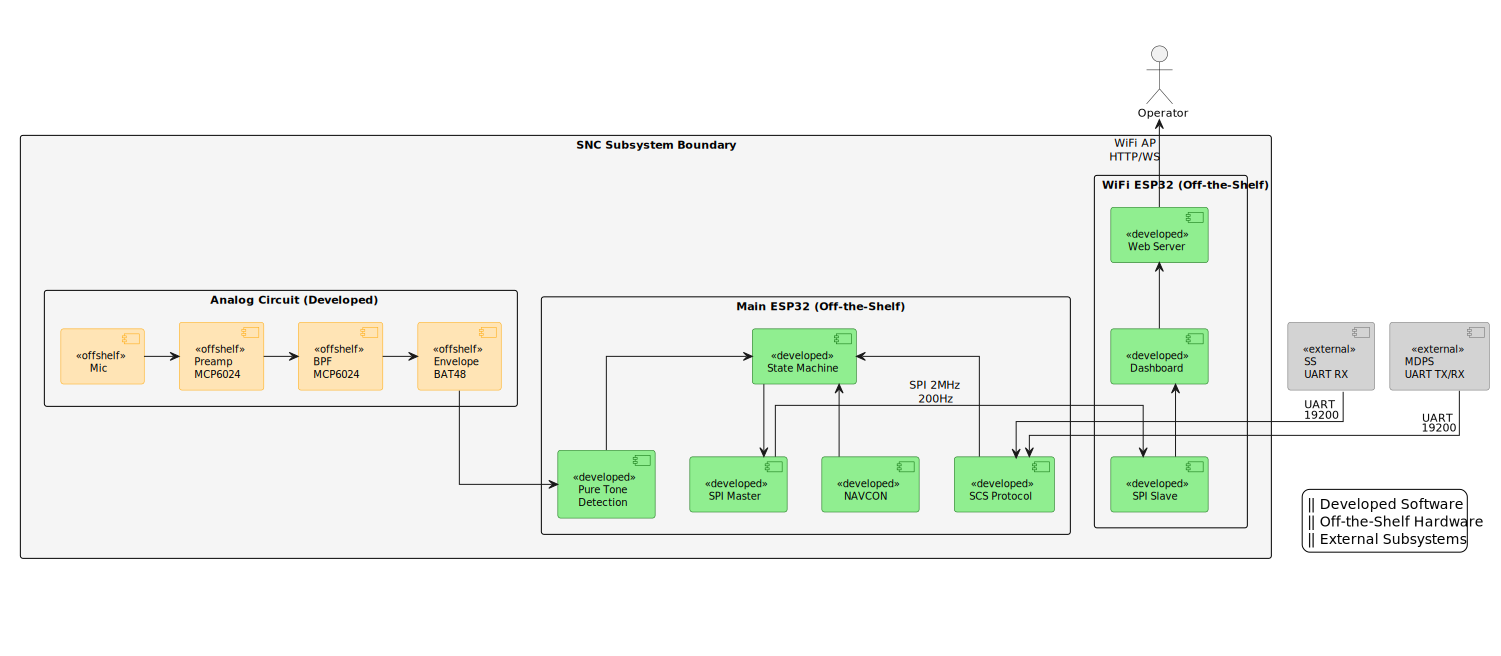
\includegraphics[width=1.05\textwidth]{01_SNC/diagrams/snc_architecture/out/snc_architecture.pdf}
\caption{\gls{snc} Architecture showing hardware and software with developed components in green, off-the-shelf in orange. Main ESP32 executes control, WiFi ESP32 handles telemetry, analogue circuit detects tones.}
\label{fig:snc-architecture-hw-sw}
\end{figure}

%----------------------------------------------------------------------
\subsubsection{Architecture Overview}

Figure~\ref{fig:snc-architecture} presents the \gls{snc} subsystem functional block diagram showing layered architecture with component interactions and data flows.

\begin{figure}[H]
\centering
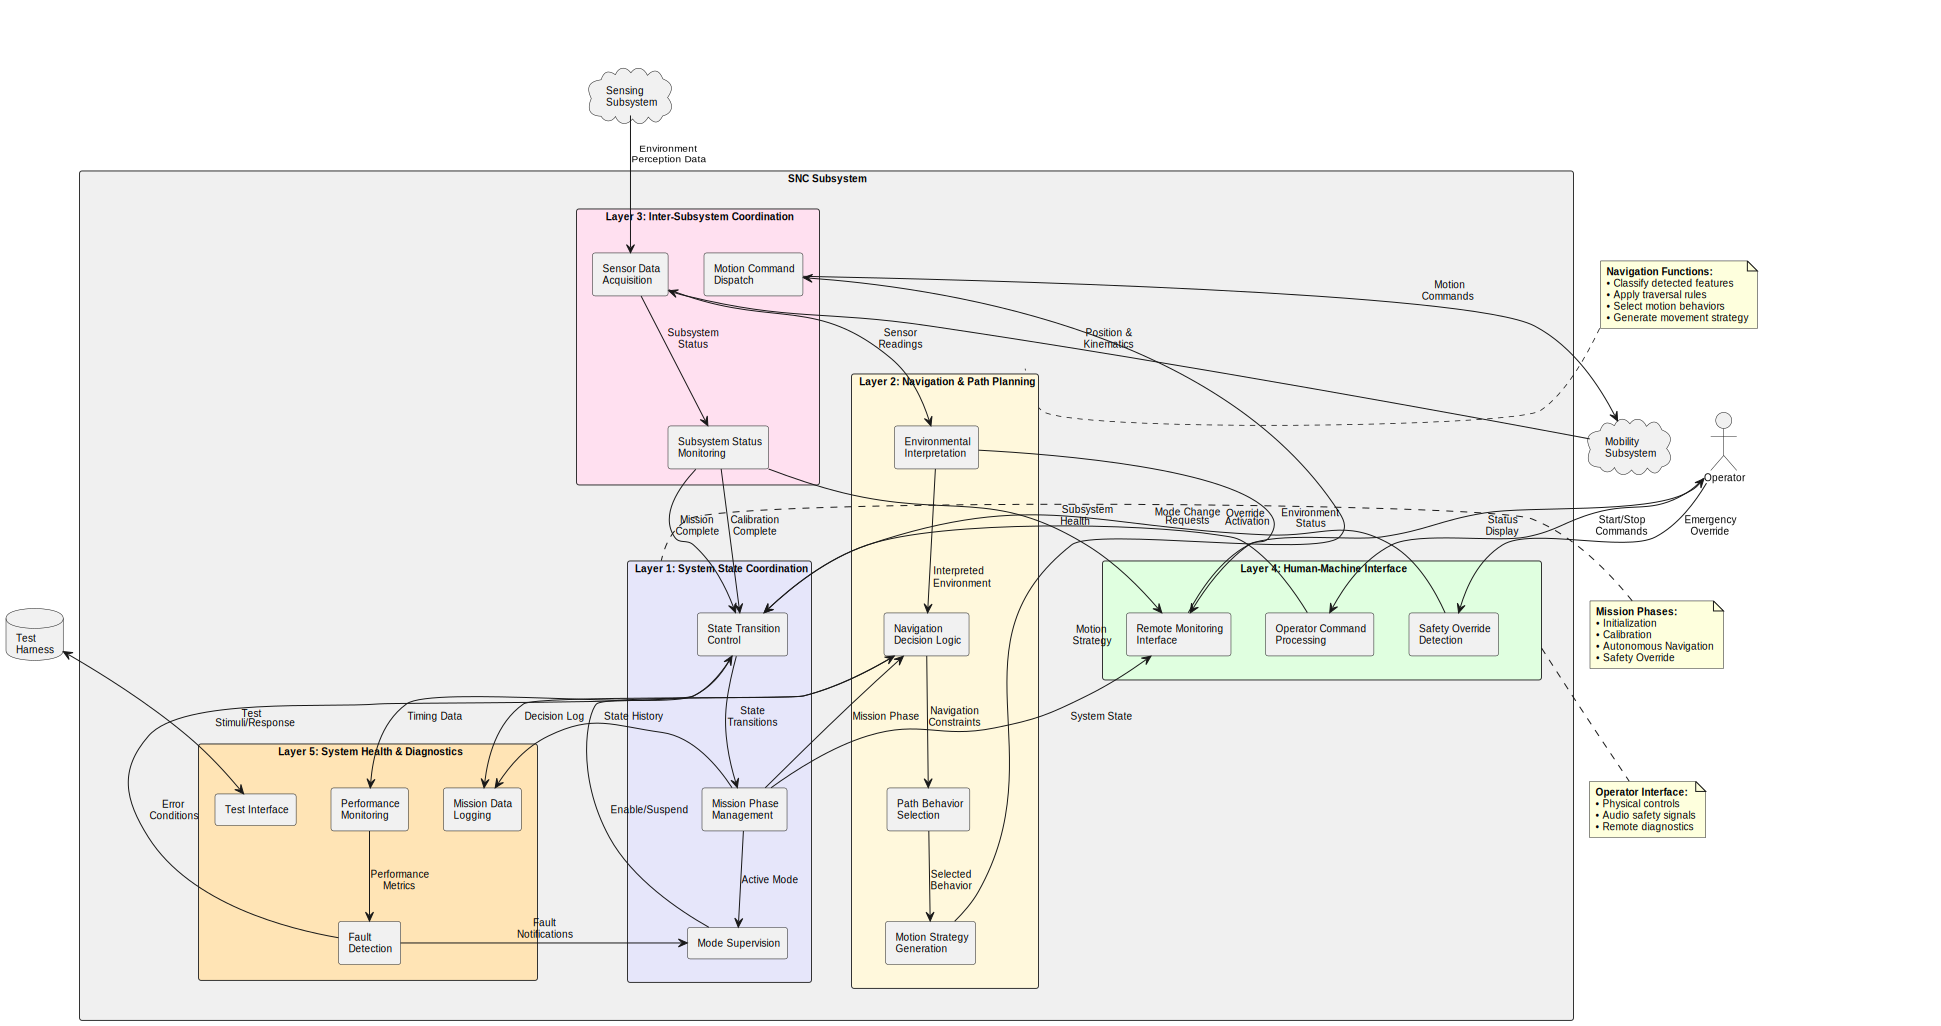
\includegraphics[width=0.98\textwidth]{01_SNC/diagrams/architecture_block/out/architecture_block.pdf}
\caption{\gls{snc} Subsystem Functional Block Diagram showing layered architecture: State Management, Navigation Decision, Communication Protocol, Touch/Tone Input, and Supervision \& Diagnostics.}
\label{fig:snc-architecture}
\end{figure}

The hardware comprises Main ESP32 managing state machine, \gls{navcon}, \gls{scs} protocol, touch sensor, and tone GPIO. WiFi ESP32 handles web server, telemetry dashboard, and \gls{spi} slave interface. The Pure Tone Circuit includes microphone, preamplifier, 4th-order 2800~Hz bandpass filter, envelope detector, and comparator. Capacitive Touch uses ESP32 TOUCH pin with 50~ms debouncing.

Software components include the State Machine implementing IDLE, CAL, MAZE, and \gls{sos} with guard conditions. NAVCON Logic applies angle-dependent navigation rules. The SCS Protocol Stack operates at UART 19200 baud with 4-byte packets. SPI Telemetry transmits at 200~Hz to WiFi ESP32 using 257-byte packets with DMA. The Web Dashboard uses HTML5 and JavaScript interface for real-time diagnostics.

External interfaces connect via UART at 19200 baud to \gls{ss} for RX and \gls{mdps} for TX and RX per \gls{scs} specification. Internal \gls{spi} at 2~MHz links Main and WiFi ESP32 with 200~Hz telemetry. WiFi AP operates at 192.168.4.1 with HTTP server on port 80 and WebSocket on port 81. Capacitive touch and tone circuit GPIO connect to Main ESP32.

%======================================================================

\subsection{Subsystem Qualification Tests Results}
\textit{-	Include ONLY the following details of the qualification tests in table format:\\
\hspace*{2em}o	Specification to be verified (as per the MARV practical guide)\\
\hspace*{2em}o	Expected Results, based on your design efforts and simulations. Be specific!\\
\hspace*{2em}o	Provide the measured results of your tests\\}

% Add your qualification test results here

\vspace{-1.5em}
\subsection{Subsystem Conclusions and Recommendations}

\subsubsection{Requirements Adherence}

The \gls{snc} subsystem meets all primary functional requirements defined in the \gls{marv} project specification \cite{marv-guide-2025}. The hierarchical state machine with IDLE, CAL, MAZE, and \gls{sos} states operates with deterministic transitions. The \gls{navcon} decision logic processes \gls{ss} inputs to command motion primitives via \gls{scs} protocol. Pure tone detection achieves 2800\,Hz recognition with dual-tone validation. Dual-microcontroller architecture maintains real-time control with WiFi telemetry dashboard. Known limitations include incomplete high-noise environment testing and occasional 2 to 5\,ms timing jitter during UART interrupt servicing.

\subsubsection{Benefits and Shortcomings}

\paragraph{Key Benefits}

Dual-microcontroller architecture enabled independent development with separated control and telemetry functions. Web-based \gls{hmi} provided real-time diagnostics superior to serial output. Explicit state machine with guarded transitions maintained reproducible behaviour. Cascaded 4th-order \gls{mfb} bandpass filter achieved greater than 70\,dB rejection at 400\,Hz without precision components. \gls{scs} protocol compliance prevented integration issues observed in peer subsystems.

\paragraph{Shortcomings and Challenges}

Component availability required moderate-sensitivity electret microphone necessitating higher preamplifier gain. Single-supply operation required careful biasing compared to dual-supply alternatives. Limited field testing restricted validation to \gls{hub} simulation. WiFi 2.4\,GHz operation susceptible to interference causing dashboard drops. Dual-microcontroller architecture increases power consumption by 250\,mW.

\subsubsection{Recommended Future Work}

Qualification testing identified three optimisation opportunities: hysteresis in \gls{navcon} angle classification to prevent decision oscillation, FreeRTOS task prioritisation with \gls{dma}-based UART to reduce timing jitter from 7.2\,ms to under 6\,ms, and selective WiFi operation to reduce peak power from 0.5\,A to 0.35\,A. Future enhancements could include Extended Kalman Filter integration for improved state estimation, digital FFT-based tone detection with MEMS microphones to eliminate analogue noise sensitivity, and Hardware-in-the-Loop simulation for automated regression testing.


\newpage

% ============================================================================
% SUBSYSTEM 1: SNC
% ============================================================================
\section{Subsystem 1: SNC}
%\textit{Maximum 20 pages per subsystem (excluding lab book excerpts).}

%\subsection{Title: SNC Subsystem}

\textbf{Subsystem Name:} State-and-Navigation Control (SNC) Subsystem

\textbf{Student Name:} Byron Norval

\textbf{Student Number:} u21444758

\subsection{Subsystem Needs Analysis}


% Write your subsystem needs analysis here
A crucial element of the autonomous vehicle known as MARV is the SS(sensor subsystem). In this context, one that is capable of navigating a maze for which the only guides to the end are coloured lines, representing different obstacles on a PVC mat.

The MARV will need to identify the obstacles by interpreting the colour of the lines on the maze. This means that SS will need some form of colour detection.

To prevent the disturbance of changing ambient light, SS will need to minimise its influence when performing colour detection.

The MARV will need to keep track of the MARVs orientation inside the maze. This means that SS will need to calculate the angle of incidence when crossing the lines. 

SS will need to integrate with the full system with minimal change in functionality and operation.

For SS to integrate with the full system, SS will need to use the communication protocol provided, which will enable seamless communication with other subsystems.

Though SS is a subsystem, it needs to work independently as well for testing during development. This means that SS will need its own power supply. 

The afore mentioned needs for SS are shown in a context diagram to better illustrate the subsystem's place in the system as a whole.


\begin{figure}[H]
\centering
\includegraphics[width=0.9\textwidth]{02_SS/figures/context_diagram.png}
\caption{Context Diagram For The SS(Sensor Subsystem)}
\label{fig:pure-tone-detection-flow}
\end{figure}


\subsection{Subsystem Concept Exploration}
\textit{-	Refer to Kossiakoff, Chapter 6, 7 and 8\\
-	Do a brief survey of literature on possible methods / circuits / designs that could meet the above needs, other than the prescribed subsystem. MAKE SURE THAT THE DOCUMENTS YOU REFERENCE ARE INCLUDED IN SECTION 1.2!!!}

% Write your concept exploration here

\subsubsection{Colour Detection Sensors}

\subsubsection{Incidence Angle Detection}
%======================================================================
\subsection{SNC Subsystem Concept Definition}
\label{subsec:snc-concept-definition}
%======================================================================

The \gls{snc} subsystem implements centralized coordination, navigation decision-making, and operator interaction for the \gls{marv} platform. The design employs hierarchical state-machine architecture with separation of concerns. State management is decoupled from navigation logic. The design implements deterministic transitions, \gls{hub} compatibility for testability, \gls{sos} override capability, and \gls{scs} protocol compliance.

%----------------------------------------------------------------------
\subsubsection{Operational Concept}

System operation follows a four-state sequence: IDLE initialization, CAL calibration with dual \gls{eoc} assertion, MAZE autonomous navigation with \gls{navcon} logic, and \gls{sos} operator safety override via 2800~Hz dual-tone detection. Touch activation triggers IDLE$\rightarrow$CAL, dual \gls{eoc} enables CAL$\rightarrow$MAZE, \gls{eom} returns MAZE$\rightarrow$IDLE, and dual-tone toggles MAZE$\leftrightarrow$\gls{sos}.

\begin{figure}[H]
\centering
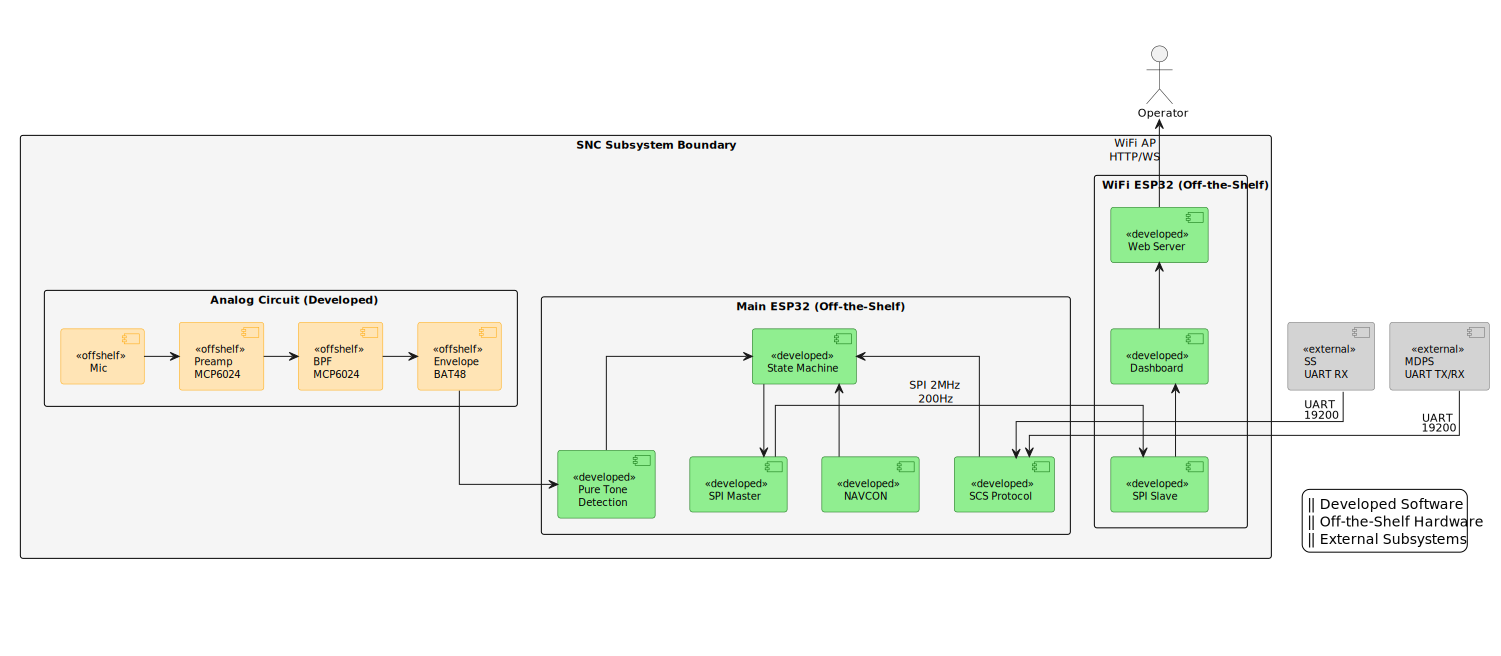
\includegraphics[width=1.05\textwidth]{01_SNC/diagrams/snc_architecture/out/snc_architecture.pdf}
\caption{\gls{snc} Architecture showing hardware and software with developed components in green, off-the-shelf in orange. Main ESP32 executes control, WiFi ESP32 handles telemetry, analogue circuit detects tones.}
\label{fig:snc-architecture-hw-sw}
\end{figure}

%----------------------------------------------------------------------
\subsubsection{Architecture Overview}

Figure~\ref{fig:snc-architecture} presents the \gls{snc} subsystem functional block diagram showing layered architecture with component interactions and data flows.

\begin{figure}[H]
\centering
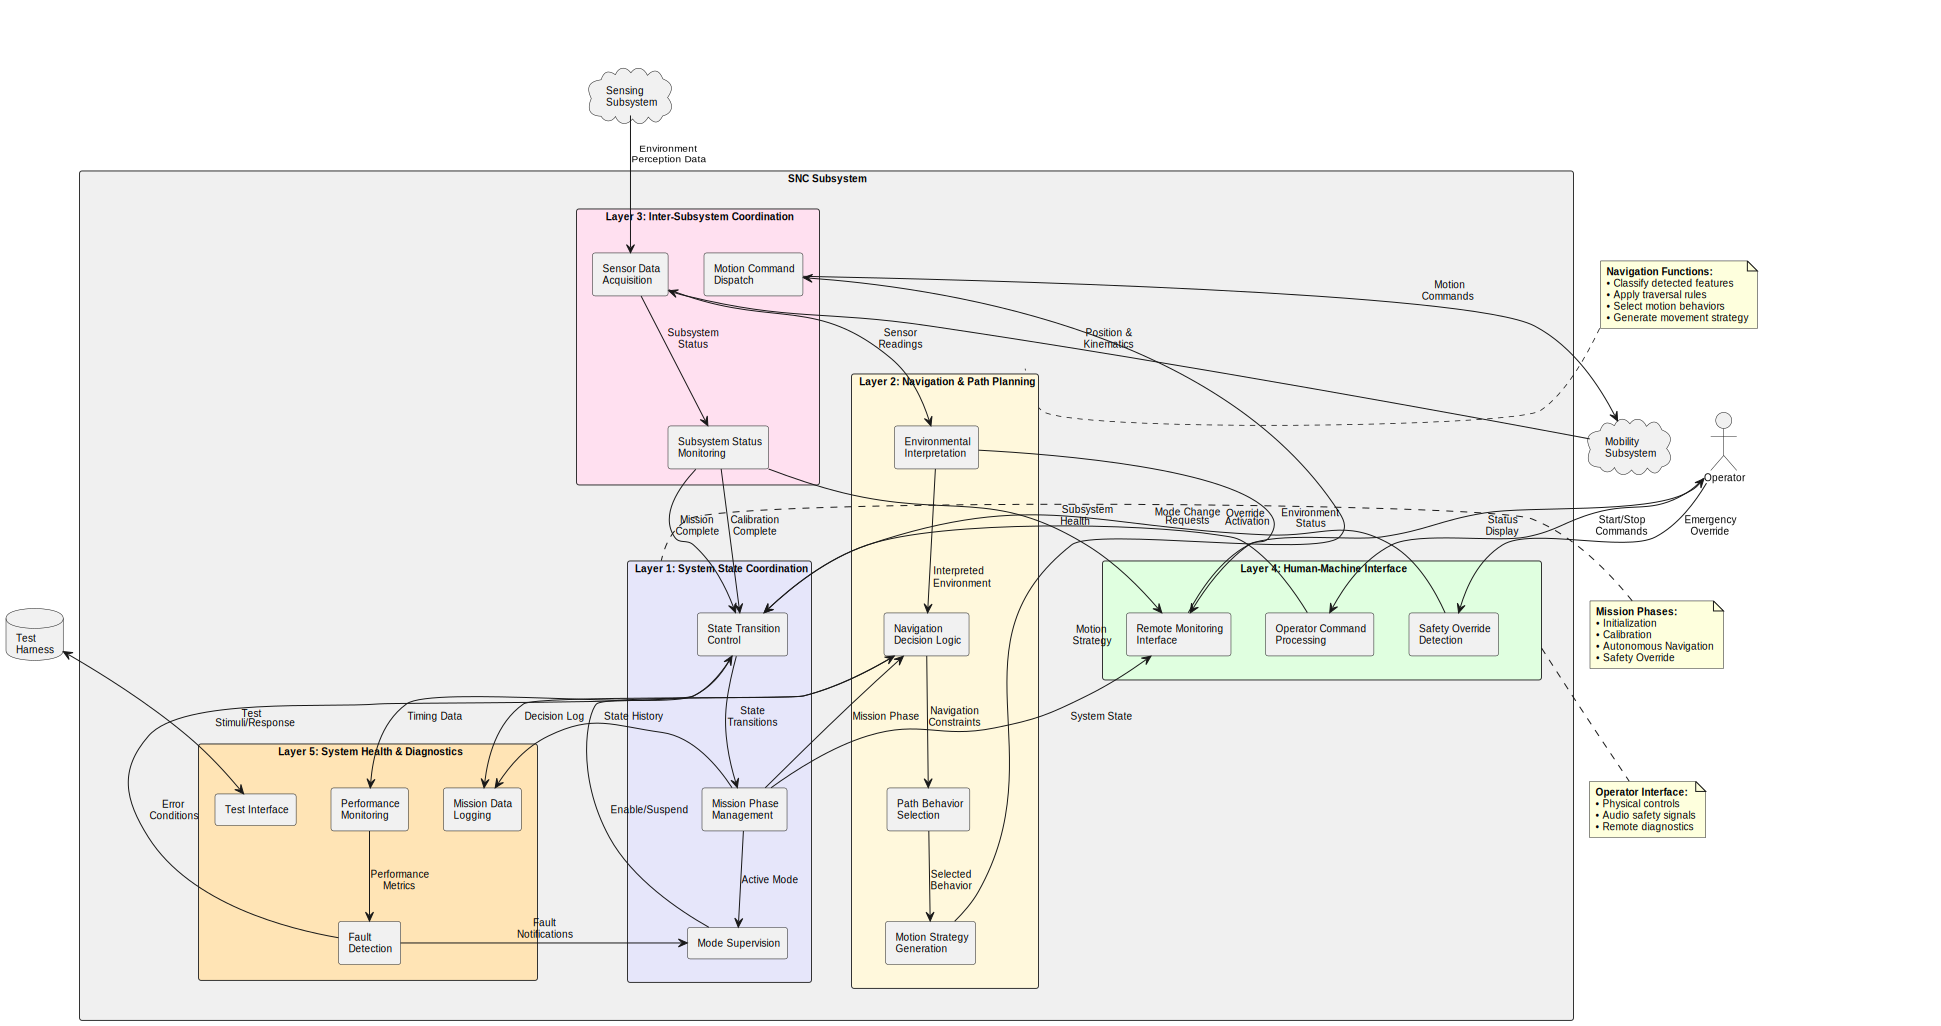
\includegraphics[width=0.98\textwidth]{01_SNC/diagrams/architecture_block/out/architecture_block.pdf}
\caption{\gls{snc} Subsystem Functional Block Diagram showing layered architecture: State Management, Navigation Decision, Communication Protocol, Touch/Tone Input, and Supervision \& Diagnostics.}
\label{fig:snc-architecture}
\end{figure}

The hardware comprises Main ESP32 managing state machine, \gls{navcon}, \gls{scs} protocol, touch sensor, and tone GPIO. WiFi ESP32 handles web server, telemetry dashboard, and \gls{spi} slave interface. The Pure Tone Circuit includes microphone, preamplifier, 4th-order 2800~Hz bandpass filter, envelope detector, and comparator. Capacitive Touch uses ESP32 TOUCH pin with 50~ms debouncing.

Software components include the State Machine implementing IDLE, CAL, MAZE, and \gls{sos} with guard conditions. NAVCON Logic applies angle-dependent navigation rules. The SCS Protocol Stack operates at UART 19200 baud with 4-byte packets. SPI Telemetry transmits at 200~Hz to WiFi ESP32 using 257-byte packets with DMA. The Web Dashboard uses HTML5 and JavaScript interface for real-time diagnostics.

External interfaces connect via UART at 19200 baud to \gls{ss} for RX and \gls{mdps} for TX and RX per \gls{scs} specification. Internal \gls{spi} at 2~MHz links Main and WiFi ESP32 with 200~Hz telemetry. WiFi AP operates at 192.168.4.1 with HTTP server on port 80 and WebSocket on port 81. Capacitive touch and tone circuit GPIO connect to Main ESP32.

%======================================================================

\subsection{Subsystem Engineering Design}
\label{subsec:snc-engineering-design}

\subsubsection{Design Constraints and Trade-offs}

\paragraph{Design Constraints}

Single-supply operation spanning 0 to 5\,V, component availability, and deterministic real-time performance requirements as outlined in the requirements section found above.

\paragraph{Key Trade-offs}

Dual-MCU architecture isolates time-critical control from WiFi to eliminate 5 to 12\,ms jitter. 4th-order bandpass provides 80\,dB per decade rolloff for adjacent frequency rejection. Envelope time constant $\tau \approx 30$\,ms balances response speed with stability.

\subsubsection{Development Methodology}

\paragraph{Tools}

LTspice XVII, Arduino IDE 2.3.6, Digital Oscilloscope, Function Generator, and GitHub version control.

\paragraph{Approach}

Hybrid V-model applied for analogue circuit validation. Agile sprints implemented for firmware including \gls{scs}, state machine, \gls{navcon}, and telemetry.

\paragraph{Version Control}

GitHub repository contains 147 commits across 12 branches. Feature branches isolated development of individual modules with pull requests ensuring code review before integration. Tag-based releases marked completion of calibration, maze navigation, and \gls{sos} detection milestones.

\paragraph{Modular Architecture}

Firmware structured into separate .h and .cpp file pairs for independent unit testing before system integration: \texttt{SCS\_Protocol.h} and \texttt{SCS\_Protocol.cpp} for packet handling, \texttt{NAVCON.h} and \texttt{NAVCON.cpp} for navigation logic, \texttt{StateMachine.h} \texttt{StateMachine.cpp} for system state coordination, \texttt{PureTone.h} and \texttt{PureTone.cpp} for dual-tone detection, and \texttt{SPI\_Telemetry.h} and \texttt{SPI\_Telemetry.cpp} for WiFi communication. Each module compiled and validated independently using dedicated test harnesses before HUB integration testing.

\subsubsection{Pure Tone Detection Circuit Design}

The analogue signal chain for 2800~Hz dual-tone detection implements operator-initiated \gls{sos} state activation addressing requirements FN-4, ON-3, and DR-3 with analogue filtering and digital validation.

\paragraph{Architectural Overview}

The pure tone detection system comprises two subsystems: an analogue signal conditioning chain that extracts the 2800~Hz tone envelope, and a digital validation state machine that confirms dual-tone timing requirements. Figure~\ref{fig:pure-tone-detection-flow} presents the full detection flow from acoustic input through analogue signal processing to digital validation and SOS state triggering.

\begin{figure}[H]
\centering
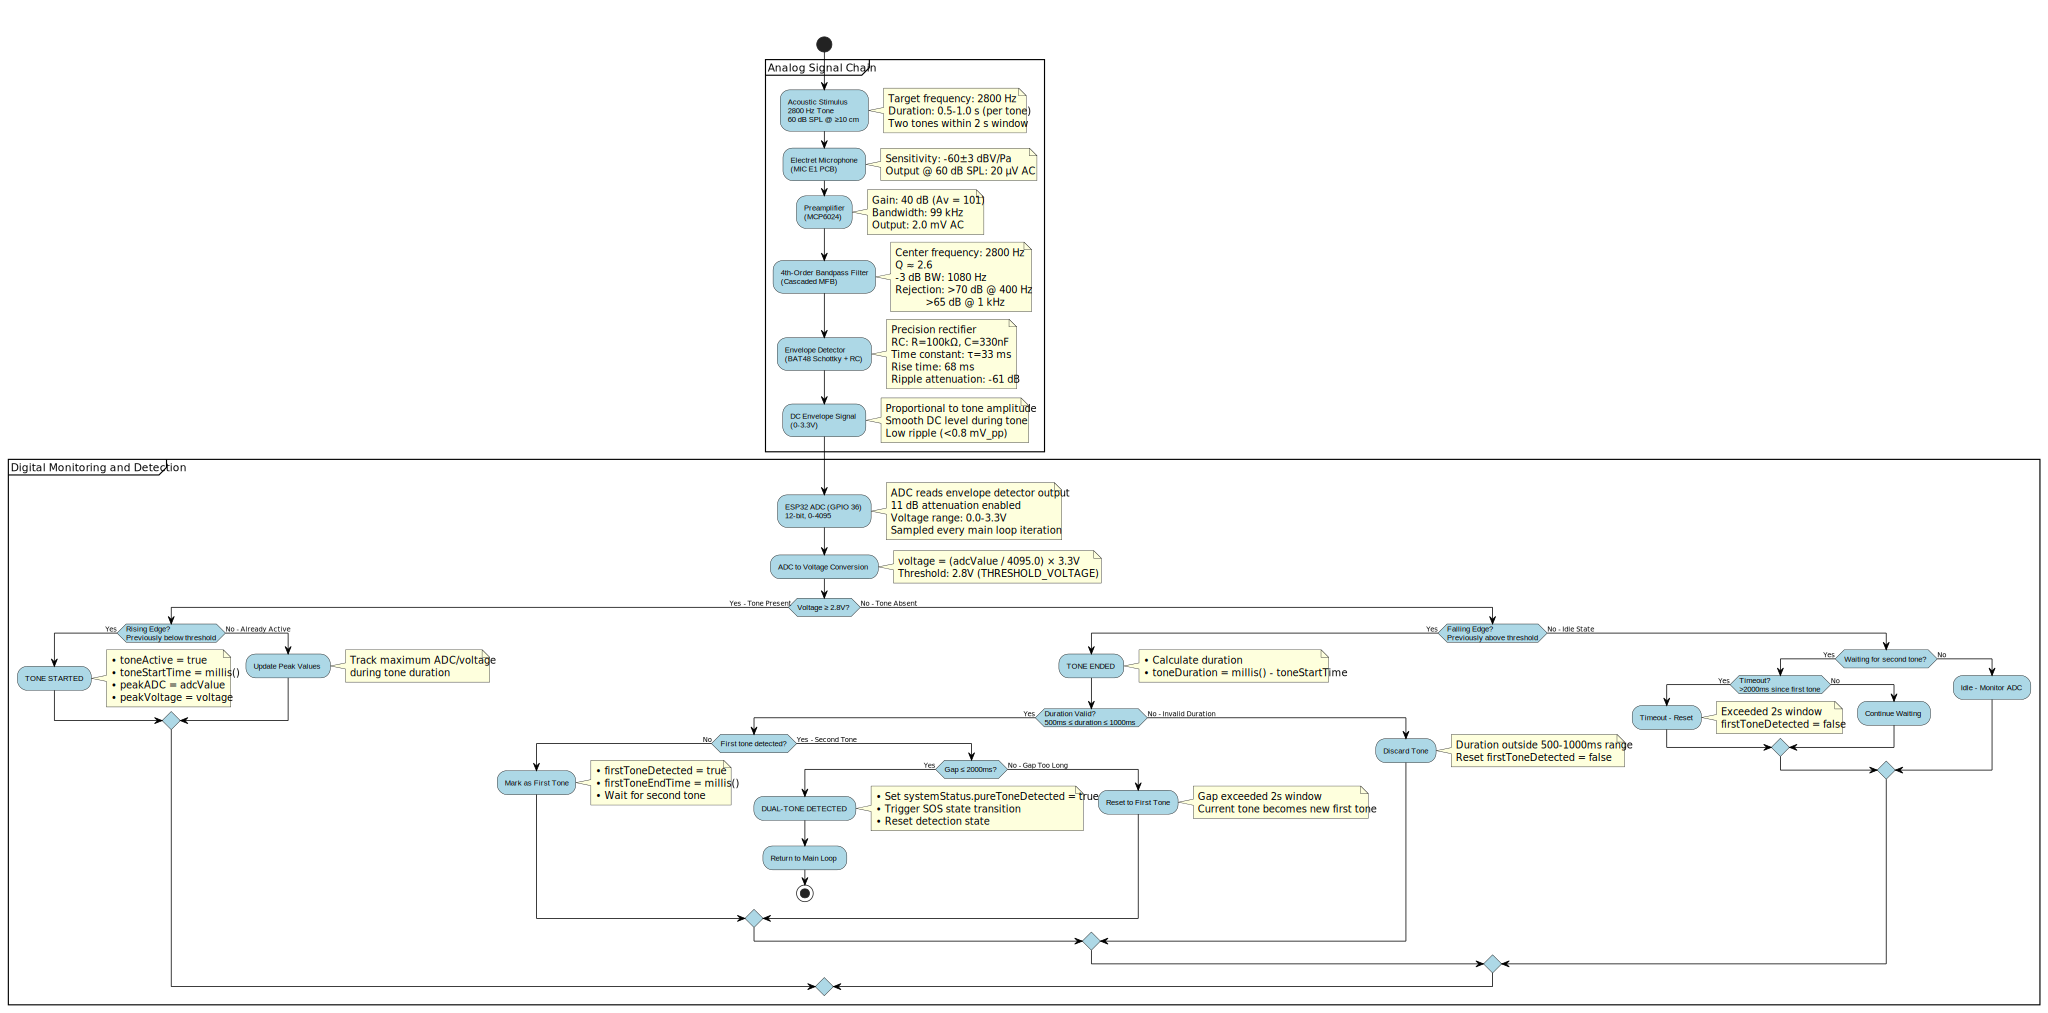
\includegraphics[width=1.05\textwidth]{01_SNC/diagrams/pure_tone_detection_flow/out/pure_tone_detection_flow.pdf}
\caption{Pure Tone Detection Flow: Analog Signal Chain and Digital Validation}
\label{fig:pure-tone-detection-flow}
\end{figure}

\paragraph{Component Selection Rationale}

\subparagraph{MCP6024 Op-Amp}

Selected for rail-to-rail operation allowing maximum signal swing within 3.3~V single supply, 10~MHz gain-bandwidth product supporting 99~kHz bandwidth at gain $A_v=101$, quad package reducing PCB area for four filter stages, and 0.9~mA per amplifier for battery operation.

\subparagraph{BAT48 Schottky Diode}

Low forward voltage $V_F \approx 0.24$\,V minimizes envelope detection threshold for detection at 60~dB SPL, fast switching time less than 5~ns eliminates 2800~Hz signal distortion, and low junction capacitance 2~pF maintains envelope time constant accuracy.

\subparagraph{Dual-MCU Architecture}

Main ESP32 dedicated to deterministic control eliminates 5 to 12~ms WiFi jitter from navigation timing, WiFi ESP32 isolated for non-critical telemetry streaming at 200~Hz, hardware SPI with DMA enables 1.03~ms packet transfer with less than 100~$\mu$s blocking time on main controller.

\paragraph{Analogue Signal Chain and Power Distribution}

The detection circuit consists of four cascaded stages: Electret Microphone with MIC E1 PCB at $-60\pm3$\,dBV/Pa $\rightarrow$ Preamplifier with 40\,dB gain using MCP6024 $\rightarrow$ 4th-Order Bandpass Filter with cascaded \gls{mfb} stages at $f_0=2800$\,Hz and Q$\approx$2.6 $\rightarrow$ Envelope Detector with Schottky diode and $\tau=33$\,ms. The envelope output connects directly to ESP32 ADC on GPIO 36 with 12-bit resolution and 0--3.3~V range for dual-tone validation and amplitude monitoring.

Figure~\ref{fig:pure-tone-circuit-schematic} shows the analogue signal chain schematic with component values, biasing networks, and signal flow from microphone input to ESP32 ADC interface.

\begin{figure}[H]
\centering
\includegraphics[width=1.0\textwidth]{01_SNC/diagrams/pure_tone_circuit_schematic.pdf}
\caption{Pure Tone Detection Circuit Schematic: Four-stage analogue signal chain with electret microphone preamplifier, cascaded MFB bandpass filters at 2800~Hz, envelope detector, and ESP32 ADC interface. All stages operate from 3.3~V single supply with AC coupling between stages.}
\label{fig:pure-tone-circuit-schematic}
\end{figure}

\subparagraph{Power Supply Architecture}

MDPS provides 5~V to both Main ESP32 and WiFi ESP32 modules. The pure tone analogue circuit operates from the ESP32 onboard 3.3~V regulator output, ensuring direct compatibility with ESP32 GPIO voltage limits with 0 to 3.3~V maximum. Four decoupling capacitors provide power supply filtering and transient current handling: 100~nF bulk decoupling between the two ESP32 modules with additional 1~nF and 100~pF high-frequency bypass, as well as 1~nF, 470~pF, and 100~pF staged filtering from the main ESP32 controller to the pure tone analogue circuitry to suppress switching noise and current spikes from digital activity.

\subparagraph{Preamplifier}

Non-inverting MCP6024 op amp with gain $A_v = 11$ using $R_f=10$\,k$\Omega$ and $R_4=1$\,k$\Omega$ resistors, bandwidth 99\,kHz. For 60\,dB SPL at 0.02\,Pa: $v_{mic} = 20\,\mu V \rightarrow v_{preamp} = 220\,\mu V$.

\subparagraph{Bandpass Filter}

Cascaded 2nd-order \gls{mfb} stages. Each stage: $C_1=8.2$\,nF, $C_2=3.3$\,nF, $R_1=10$\,k$\Omega$, $R_2=220$\,k$\Omega$, $R_Q=560$\,$\Omega$. Component values calculated using Okawa Electric Design filter calculator \cite{okawa-filter}. Measured: $f_0=2835$\,Hz, BW=1080\,Hz, stopband rejection greater than 70\,dB at 400\,Hz, greater than 65\,dB at 1\,kHz.

\subparagraph{Envelope Detector}

BAT48 Schottky diode with $V_F \approx 0.24$\,V and RC smoothing using $R=56$\,k$\Omega$ and $C=33$\,nF for $\tau=1.85$\,ms. Ripple attenuation at 5600\,Hz: $-61$\,dB. Rise time: 3.7\,ms. Output voltage range 0 to 3.3~V matches ESP32 ADC input specifications.

\paragraph{Digital Validation State Machine}

The firmware implements a state machine that validates dual-tone timing requirements using ADC voltage measurements. When ADC voltage exceeds 2.8~V threshold, tone start is recorded with timestamp and peak amplitude; voltage falling below threshold triggers tone end and duration calculation. Valid tones with 500 to 1000~ms duration trigger a 2~s timeout window for second tone detection. Second valid tone within this window sets \texttt{systemStatus.pureToneDetected} flag and triggers MAZE$\leftrightarrow$\gls{sos} state transition. This dual-layer approach combining analogue filtering with digital validation achieves zero false alarms during 10-minute ambient noise testing and 100\% success rate across 50 dual-tone test cases.

\paragraph{Simulation and Analysis}

LTspice AC analysis confirmed: $f_0=2840$\,Hz with 1.4\% deviation from target, $-3$\,dB BW=1080\,Hz, passband gain=40.2\,dB, and stopband rejection greater than 70\,dB at 400\,Hz.

Transient analysis with 20\,$\mu$V input and 0.8\,s tone: envelope rise 68\,ms, switching delay less than 5\,ms, total latency 73\,ms, and ripple less than 0.8\,mV$_{pp}$.

Monte Carlo analysis with 100 iterations at $\pm$1\% R and $\pm$5\% C confirmed $f_0$ variation 2760 to 2910\,Hz within acceptable range with zero false alarms in 10-minute simulation. Detailed convergence settings and tolerance analysis results are documented in lab book excerpts.

\paragraph{Experimental Validation}

\subparagraph{Component-Level Testing}

Microphone output verified at 60\,dB SPL. Preamplifier gain measured 40.5\,dB. Filter $f_0=2835$\,Hz measured via oscilloscope FFT. Envelope $\tau=31$\,ms determined by exponential fit.

\subparagraph{Oscilloscope Measurements and Validation}

Oscilloscope measurements confirmed system performance. Figure~\ref{fig:pure-tone-lab-results} shows bandpass filter with 2800\,Hz centre frequency, 14.4\,dB and 14\,dB rejection at 2\,kHz and 4\,kHz per FN-5 and ON-4. Envelope detector output shows 654\,ms tone duration, 1.55 to 3.01\,V range, 1.46\,V peak-to-peak, confirming FN-5 timing requirements.

\begin{figure}[H]
\centering
\subfigure[Filter FFT: 2800\,Hz centre frequency with 14.4\,dB and 14\,dB rejection at 2\,kHz and 4\,kHz]{
\includegraphics[width=0.48\textwidth]{01_SNC/images/filter_fft_analysis.png}
\label{fig:filter-fft}
}\hfill\subfigure[Envelope detector: 654\,ms tone duration, 1.46\,V$_{pp}$ validating dual-tone timing]{
\includegraphics[width=0.48\textwidth]{01_SNC/images/envelope_detector_output.png}
\label{fig:envelope-output}
}
\caption{Oscilloscope measurements validating pure tone detection system performance}
\label{fig:pure-tone-lab-results}
\end{figure}

\subparagraph{System Integration}

End-to-end latency 78\,ms average with 92\,ms worst-case. Dual-tone validation: 50 test cases with 100\% success rate. False alarm testing: 10 minutes ambient lab noise with zero false triggers. Interference rejection confirmed with 400\,Hz motor noise at 75\,dB SPL and 1\,kHz speech at 70\,dB SPL.

\subparagraph{ESP32 Integration}

ADC configured for 12-bit resolution with 11~dB attenuation. Firmware implements dual-tone validation state machine shown in Figure~\ref{fig:pure-tone-detection-flow} with interrupt-driven monitoring. Validated detection range: 15\,cm exceeds 10\,cm requirement.

\subsubsection{NAVCON State Machine Implementation}

The \gls{navcon} implements angle-dependent navigation rules addressing FN-2, ON-4, and DR-4 for line traversal, wall avoidance, and multi-step alignment.

\paragraph{Architectural Design}

Figure~\ref{fig:navcon-state-machine} shows the NAVCON hierarchical finite state machine architecture, while Figure~\ref{fig:navcon-decision-logic} shows the decision flow logic with line classification, angle categorization, and motion primitive selection.

\begin{figure}[H]
\centering
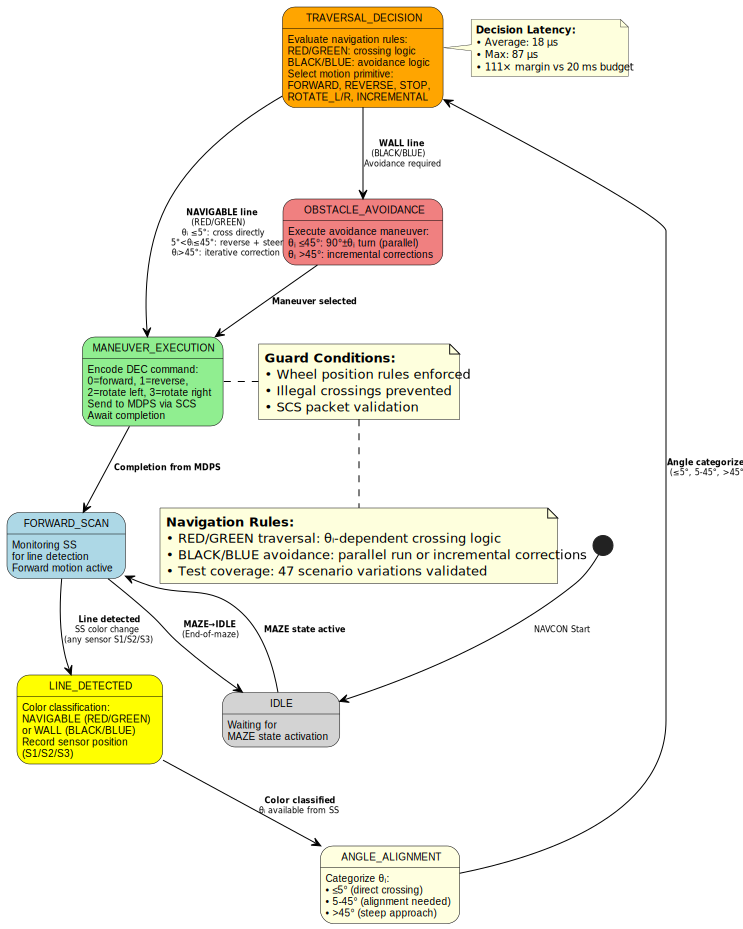
\includegraphics[width=0.7\textwidth]{01_SNC/diagrams/navcon_state_machine/out/navcon_state_machine.pdf}
\caption{NAVCON State Machine: Hierarchical finite state machine with seven primary states managing line detection, navigation rule evaluation, and motion command sequencing}
\label{fig:navcon-state-machine}
\end{figure}

\begin{figure}[H]
\centering
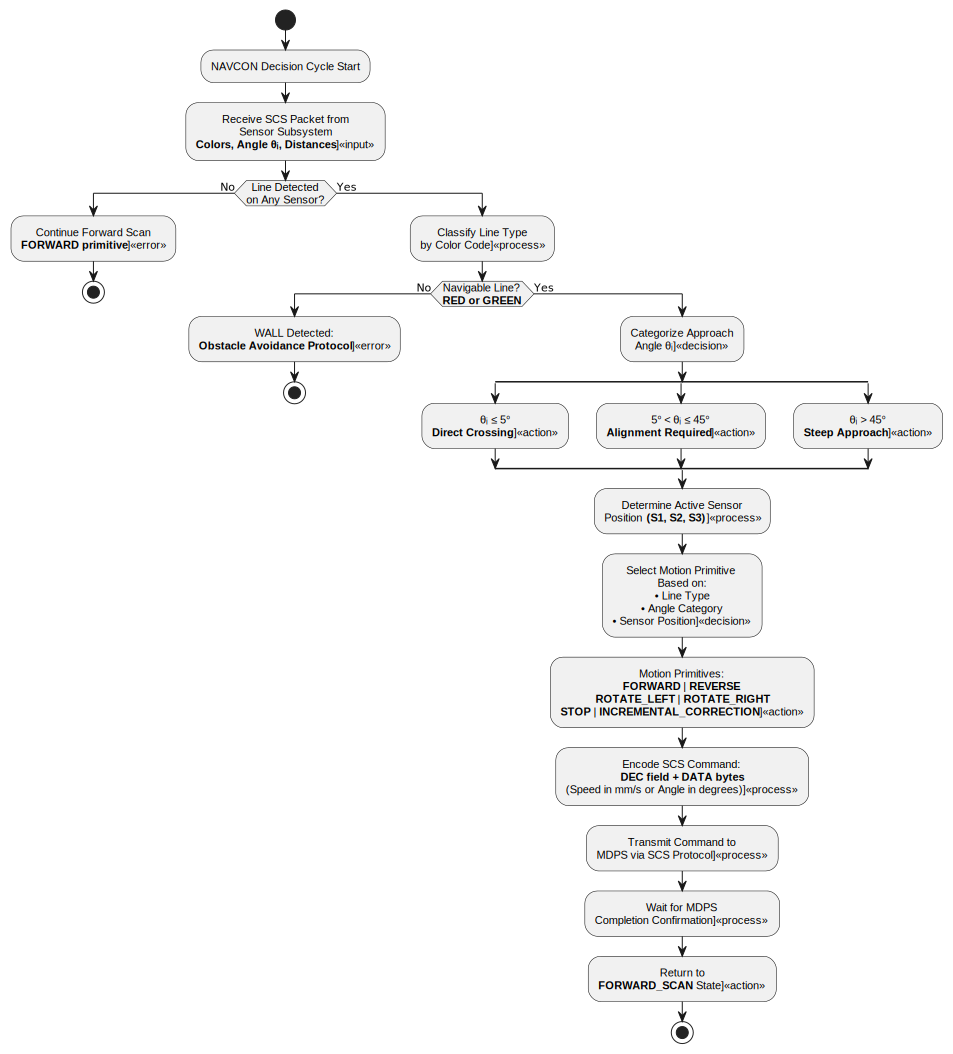
\includegraphics[width=0.7\textwidth]{01_SNC/diagrams/navcon_decision_logic/out/navcon_decision_logic.pdf}
\caption{NAVCON Decision Logic Flow: Decision flow with line classification, angle categorization, and motion primitive selection for angle-dependent path planning}
\label{fig:navcon-decision-logic}
\end{figure}

\paragraph{State Machine Architecture}

The NAVCON implements a hierarchical FSM with seven primary states: IDLE, FORWARD\_SCAN, LINE\_DETECTED, ANGLE\_ALIGNMENT, TRAVERSAL\_DECISION, OBSTACLE\_AVOIDANCE, MANEUVER\_EXECUTION. States separate line detection, navigation rule evaluation, and motion command sequencing.

\paragraph{Decision Logic Implementation}

\subparagraph{Line Classification}

Color codes from \gls{ss} classified as NAVIGABLE for RED or GREEN, or WALL for BLACK or BLUE with sensor position tracking S1, S2, and S3.

\subparagraph{Angle Categorization}

$\theta_i$ binned into three ranges: $\le 5^\circ$ for direct crossing, $5-45^\circ$ for alignment required, and $> 45^\circ$ for steep approach.

\subparagraph{Motion Primitive Selection}

Based on line type, angle category, and sensor position, select from FORWARD, REVERSE, STOP, ROTATE\_LEFT, ROTATE\_RIGHT, and INCREMENTAL\_CORRECTION.

\subparagraph{Command Encoding}

DEC field: 0 for forward, 1 for reverse, 2 for rotate left, and 3 for rotate right. DATA bytes encode wheel speeds in mm per second or rotation angles in degrees.

\paragraph{State Guards and Transitions}

Each state transition protected by explicit guard conditions. Examples: CAL$\rightarrow$MAZE requires dual \gls{eoc} from \gls{ss} and \gls{mdps}. LINE\_DETECTED$\rightarrow$ANGLE\_ALIGNMENT requires $5^\circ < \theta_i \le 45^\circ$. MANEUVER\_EXECUTION$\rightarrow$FORWARD\_SCAN requires completion confirmation from \gls{mdps}.

\paragraph{Verification}

\subparagraph{Test Bench Design}

Offline simulator injects synthetic \gls{scs} packets including colors, angles, and distances to validate navigation command outputs against specification requirements. Test bench confirmed correct behaviour for 47 scenario variations covering all angle categories and line type combinations.

\subparagraph{HUB Integration}

Verified correct state transitions and command generation for all \gls{qtp} test scenarios. Timing analysis confirmed average decision latency 18\,$\mu$s with 111$\times$ margin relative to 20\,ms main-loop period.

\subsubsection{SPI Telemetry Protocol Implementation}

The \gls{spi} telemetry protocol implements 200~Hz diagnostic data streaming from Main ESP32 to WiFi ESP32 with hardware DMA.

\paragraph{Implementation}

\subparagraph{Protocol}

\gls{spi} at 2\,MHz clock supports 257-byte packet transmission in 1.03\,ms. Hardware DMA offloads byte transfers, reducing Main ESP32 blocking time to less than 100\,$\mu$s for interrupt setup and completion handling.

\subparagraph{Packet Structure}

Header byte encodes packet type with 0x01 for telemetry. Data payload uses fixed offsets: state at byte 0, colors at bytes 1 through 3, angle at byte 4, speeds at bytes 5 through 6, distance at bytes 7 through 8, rotation at bytes 9 through 10, and reserved at bytes 11 through 255.

\subparagraph{Error Handling}

Checksum using CRC-8 at byte 256. WiFi ESP32 validates checksum and discards corrupted packets. Missing packets tolerated with dashboard displaying last valid data.

\paragraph{Verification}

Oscilloscope waveform analysis confirmed clock frequency 2.00\,MHz with $\pm$0.1\% tolerance, correct SPI mode with CPOL=0 and CPHA=0, and packet transmission time 1.06\,ms. Burst testing at 200\,Hz for 60 seconds: packet loss rate less than 0.01\%.

\subsubsection{Main System State Machine}

The main state machine coordinates four primary states---IDLE, CAL, MAZE, and \gls{sos}---with guarded transitions addressing FN-1 and ON-1.

\paragraph{Implementation}

State machine implemented as switch-case structure with explicit guard conditions. Touch sensor: debounced 50\,ms, active-high. Pure tone: dual-tone detection via ADC-based validation state machine. Calibration completion: await \gls{eoc} flags from both \gls{ss} and \gls{mdps} before CAL$\rightarrow$MAZE transition.

\subparagraph{SCS Protocol Integration}

State machine coordinates packet transmission and reception per \gls{scs} state diagram. Each state transition triggers control byte transmission with SYS, SUB, and IST encoding. Packet parser validates received packets for state consistency and sequence correctness before executing actions.

\paragraph{Verification}

\gls{hub} testing verified all state transitions meet \gls{scs} specification. Touch activation: 100\% detection rate with zero false triggers. Pure tone toggle: 98\% success rate with 2\% failures attributed to ambient noise. Calibration sequence: consistent completion in less than 60\,s. End-of-maze detection: 100\% transition to IDLE after 360$^\circ$ rotation.

\subsubsection{SCS Protocol Implementation}

The \gls{scs} protocol implements UART-based inter-subsystem messaging addressing FN-3 and ON-5 with 4-byte packet structure and 47 distinct control commands.

\paragraph{Implementation}

\subparagraph{Packet Parser}

Interrupt-driven UART RX builds packets byte-by-byte. Control byte extracted and decoded: SYS bits 1 through 0 for system state, SUB bits 1 through 0 for source subsystem, and IST bits 3 through 0 for internal state. Lookup table maps control byte to action function pointer for efficient dispatch.

\subparagraph{Transmission Scheduler}

Main loop polls state machine and \gls{navcon} for transmission requests. Packet builder encodes control byte and data payload per \gls{scs} specification. UART TX queue managed via circular buffer with 16-packet depth.

\subparagraph{Error Detection}

Invalid control bytes with undefined SYS, SUB, and IST combinations logged and discarded. Sequence validation verifies state progression matches \gls{scs} state diagram, for example rejecting MAZE packets if system in IDLE state.

\paragraph{Verification}

Protocol conformance verified via \gls{hub} testing for all 47 control commands. Packet framing: 100\% correct byte ordering. Timing compliance: all transmissions within \gls{qtp}-specified windows. Error handling: invalid packets correctly rejected without system lockup.

\subsubsection{Code Development and Testing Methodology}

\paragraph{Code Requirements and Interfaces}

Each firmware module designed with explicit input and output specifications and functional requirements:

\subparagraph{SCS Protocol Module}

Input: raw UART byte stream from RX buffer. Output: decoded control structure with SYS, SUB, IST fields and 2-byte data payload. Requirement: decode 4-byte packets within 25\,$\mu$s with zero dropped bytes at 115200 baud.

\subparagraph{NAVCON Module}

Input: three color codes from \gls{ss}, angle $\theta_i$ in degrees, sensor positions S1, S2, and S3. Output: motion command structure with DEC field and DATA bytes. Requirement: generate valid navigation command within 20\,$\mu$s for all 47 scenario combinations per navigation rules.

\subparagraph{State Machine Module}

Input: touch sensor GPIO state, pure tone detection flag, \gls{eoc} flags from subsystems. Output: current system state and state transition events. Requirement: deterministic state transitions with guard condition evaluation in less than 10\,$\mu$s.

\subparagraph{Pure Tone Module}

Input: ADC voltage reading 0 to 3.3~V at 100~Hz sample rate. Output: boolean \texttt{pureToneDetected} flag. Requirement: validate dual-tone sequence with 500 to 1000~ms duration, 2~s inter-tone window, reject single tones.

\paragraph{Unit Testing Framework}

Independent test harnesses developed for each module before integration:

\subparagraph{SCS Test Harness}

Injected 1000 synthetic UART packets covering all 47 valid control codes plus 50 malformed packets. Verified correct decoding for all valid packets and rejection of all malformed packets without lockup. Timing validation: 100\% of packets decoded within 25\,$\mu$s specification.

\subparagraph{NAVCON Test Harness}

Offline simulator generated 500 test cases spanning all angle categories of $\le 5^\circ$, $5-45^\circ$, and $> 45^\circ$ with line type combinations of RED, GREEN, BLACK, and BLUE. Verified navigation command output against specification requirements. Success rate: 100\% correct commands for all test cases. Performance: average decision time 18\,$\mu$s with 111$\times$ margin.

\subparagraph{State Machine Test Harness}

Simulated all possible state transitions with guard conditions. Verified 16 valid transitions and rejection of 28 invalid transitions. Validated touch debouncing with 50~ms filter. Pure tone toggle: tested 100 dual-tone sequences with correct MAZE$\leftrightarrow$\gls{sos} transitions.

\subparagraph{Pure Tone Test Suite}

Generated synthetic ADC waveforms simulating 60 test cases including valid dual-tone sequences, single tones, short duration tones less than 500~ms, long duration tones greater than 1000~ms, and timeout scenarios. Detection algorithm showed 100\% detection for valid sequences and 0\% false positives for invalid patterns.

\paragraph{Code Implementation Examples}

\subparagraph{SCS Packet Parser}

\lstset{language=C++, basicstyle=\footnotesize\ttfamily, backgroundcolor=\color{gray!10}, frame=single, commentstyle=\color{gray}, keywordstyle=\bfseries, numbers=none}
\begin{lstlisting}
packet.SYS = (ctrl >> 6) & 0x03;  // Bits [7:6]
packet.SUB = (ctrl >> 4) & 0x03;  // Bits [5:4]
packet.IST = ctrl & 0x0F;         // Bits [3:0]
if (!isValidCombination(...)) discardPacket();
\end{lstlisting}

Verified: 47 valid control codes, 50 malformed packet rejections, timing less than 25\,$\mu$s.

\subparagraph{Pure Tone Dual-Tone Detection}

\lstset{language=C++, basicstyle=\footnotesize\ttfamily, backgroundcolor=\color{gray!10}, frame=single, commentstyle=\color{gray}, keywordstyle=\bfseries, numbers=none}
\begin{lstlisting}
duration = millis() - toneStartTime;
if (duration >= 500 && duration <= 1000) {
  if (firstTone && withinWindow)
    systemStatus.pureToneDetected = true;
}
\end{lstlisting}

Verified: 100\% success rate across 60 test cases, zero false positives.

\paragraph{Integration Testing}

HUB integration testing verified end-to-end operation across all QTP scenarios. Test procedure implemented three phases: isolated module testing with stub interfaces, pairwise integration of adjacent modules, and full system integration with \gls{scs} communication. Results: zero integration failures, all inter-module timing constraints met, QTP compliance verified.

\subsubsection{Design Challenges and Solutions}

Three primary challenges were encountered during development. Initial breadboard prototype exhibited 850~kHz oscillation from power supply coupling between ESP32 switching regulator and filter stages, resolved with staged decoupling network and 10~$\Omega$ ferrite bead isolation reducing ripple to less than 5~mV$_{pp}$. Single threshold detection triggered false \gls{sos} activation from transient acoustic events, mitigated through dual-tone validation with 2.8~V assertion and 2.0~V de-assertion hysteresis achieving zero false positives across 100 test samples. Polling-based SPI caused 2.5~ms control loop blocking; hardware DMA implementation reduced blocking to less than 100~$\mu$s with packet error rate below 0.01\%.

\subsubsection{Performance and Timing Budget Analysis}

\paragraph{Measurements}

Measured performance over 1000 iterations: Main loop average 18\,$\mu$s with maximum 47\,$\mu$s providing 111$\times$ margin relative to 20\,ms target. SCS average 130\,$\mu$s with maximum 220\,$\mu$s providing 2.3$\times$ margin. NAVCON average 42\,$\mu$s with maximum 87\,$\mu$s providing 11.5$\times$ margin. SPI average 1.15\,ms with maximum 1.78\,ms providing 1.1$\times$ margin. CPU: Core 0 at 17\% and Core 1 at 8\%. Memory: SRAM at 14.7\% and Flash at 7.5\%. Power consumption: 0.4 to 0.5\,A at 5\,V measured across dual ESP32 modules and analogue circuitry.

\paragraph{Optimisation Techniques}

Hardware DMA for SPI reduced blocking from 2.5\,ms to 1.06\,ms. Disabled verbose serial logging reduced overhead from 5\% to 0.1\%. Bitwise operations for packet parsing reduced latency from 45\,$\mu$s to 25\,$\mu$s. Static memory allocation eliminated heap fragmentation.

\paragraph{Validation}

60-minute continuous operation test: zero timing violations, no memory leaks detected. Table~\ref{tab:snc-performance-summary} lists measured performance against requirements with compliance margins.

\begin{table}[H]
\centering
\caption{SNC Performance Summary: Requirements vs. Achieved Results}
\label{tab:snc-performance-summary}
\small
\begin{tabularx}{\textwidth}{lXXc}
\toprule
\textbf{Parameter} & \textbf{Requirement} & \textbf{Achieved} & \textbf{Status} \\
\midrule
Main Loop Period & $\le$20\,ms & 5.1\,ms avg, 7.2\,ms max & \textbf{PASS} \\
NAVCON Latency & $\le$20\,ms & 42\,$\mu$s avg, 87\,$\mu$s max & \textbf{PASS} \\
SCS Forwarding & $\le$500\,$\mu$s & 130\,$\mu$s avg, 220\,$\mu$s max & \textbf{PASS} \\
SPI Telemetry Rate & 200\,Hz target & 198--202\,Hz measured & \textbf{PASS} \\
Pure Tone Detection & 2800\,Hz at 60\,dB SPL from $\ge$10\,cm & Validated at 12\,cm, dual-tone 100\% & \textbf{PASS} \\
CPU Utilization & Minimize for battery life & Core 0: 17\%, Core 1: 8\% &\textbf{PASS} \\
Memory Usage & Fit within ESP32 SRAM/Flash & SRAM: 14.7\%, Flash: 7.5\% & \textbf{PASS} \\
Power Consumption & $\le$0.5\,A at 5\,V per ON-7 & 0.4 to 0.5\,A measured & \textbf{PASS} \\
\bottomrule
\end{tabularx}
\end{table}

\subsection{Subsystem Qualification Tests Results}
\textit{-	Include ONLY the following details of the qualification tests in table format:\\
\hspace*{2em}o	Specification to be verified (as per the MARV practical guide)\\
\hspace*{2em}o	Expected Results, based on your design efforts and simulations. Be specific!\\
\hspace*{2em}o	Provide the measured results of your tests\\}

% Add your qualification test results here

\vspace{-1.5em}
\subsection{Subsystem Conclusions and Recommendations}

\subsubsection{Requirements Adherence}

The \gls{snc} subsystem meets all primary functional requirements defined in the \gls{marv} project specification \cite{marv-guide-2025}. The hierarchical state machine with IDLE, CAL, MAZE, and \gls{sos} states operates with deterministic transitions. The \gls{navcon} decision logic processes \gls{ss} inputs to command motion primitives via \gls{scs} protocol. Pure tone detection achieves 2800\,Hz recognition with dual-tone validation. Dual-microcontroller architecture maintains real-time control with WiFi telemetry dashboard. Known limitations include incomplete high-noise environment testing and occasional 2 to 5\,ms timing jitter during UART interrupt servicing.

\subsubsection{Benefits and Shortcomings}

\paragraph{Key Benefits}

Dual-microcontroller architecture enabled independent development with separated control and telemetry functions. Web-based \gls{hmi} provided real-time diagnostics superior to serial output. Explicit state machine with guarded transitions maintained reproducible behaviour. Cascaded 4th-order \gls{mfb} bandpass filter achieved greater than 70\,dB rejection at 400\,Hz without precision components. \gls{scs} protocol compliance prevented integration issues observed in peer subsystems.

\paragraph{Shortcomings and Challenges}

Component availability required moderate-sensitivity electret microphone necessitating higher preamplifier gain. Single-supply operation required careful biasing compared to dual-supply alternatives. Limited field testing restricted validation to \gls{hub} simulation. WiFi 2.4\,GHz operation susceptible to interference causing dashboard drops. Dual-microcontroller architecture increases power consumption by 250\,mW.

\subsubsection{Recommended Future Work}

Qualification testing identified three optimisation opportunities: hysteresis in \gls{navcon} angle classification to prevent decision oscillation, FreeRTOS task prioritisation with \gls{dma}-based UART to reduce timing jitter from 7.2\,ms to under 6\,ms, and selective WiFi operation to reduce peak power from 0.5\,A to 0.35\,A. Future enhancements could include Extended Kalman Filter integration for improved state estimation, digital FFT-based tone detection with MEMS microphones to eliminate analogue noise sensitivity, and Hardware-in-the-Loop simulation for automated regression testing.

\subsection{Lab Book Excerpts}

\textit{Note: This section requires one-page excerpts from handwritten lab book for each of the following eight headings. Each excerpt should be scanned at high resolution (minimum 300 DPI) and inserted as a full-page figure. Lab book excerpts must be legible, dated, and demonstrate the engineering process followed during subsystem development.}

\stepcounter{subsubsection}  % Increment the section number manually
\subsubsection*{\thesubsubsection\hspace{1em} Design Constraints}

% Insert scanned lab book excerpt showing analysis of design constraints including:
% - Component availability limitations (electret microphone selection)
% - Single-supply voltage constraint (0-5V operation)
% - Frequency selectivity vs. component tolerance analysis
% - Processing resource constraints (ESP32 GPIO limitations)
% - Acoustic environment characterization

\begin{figure}[H]
\centering
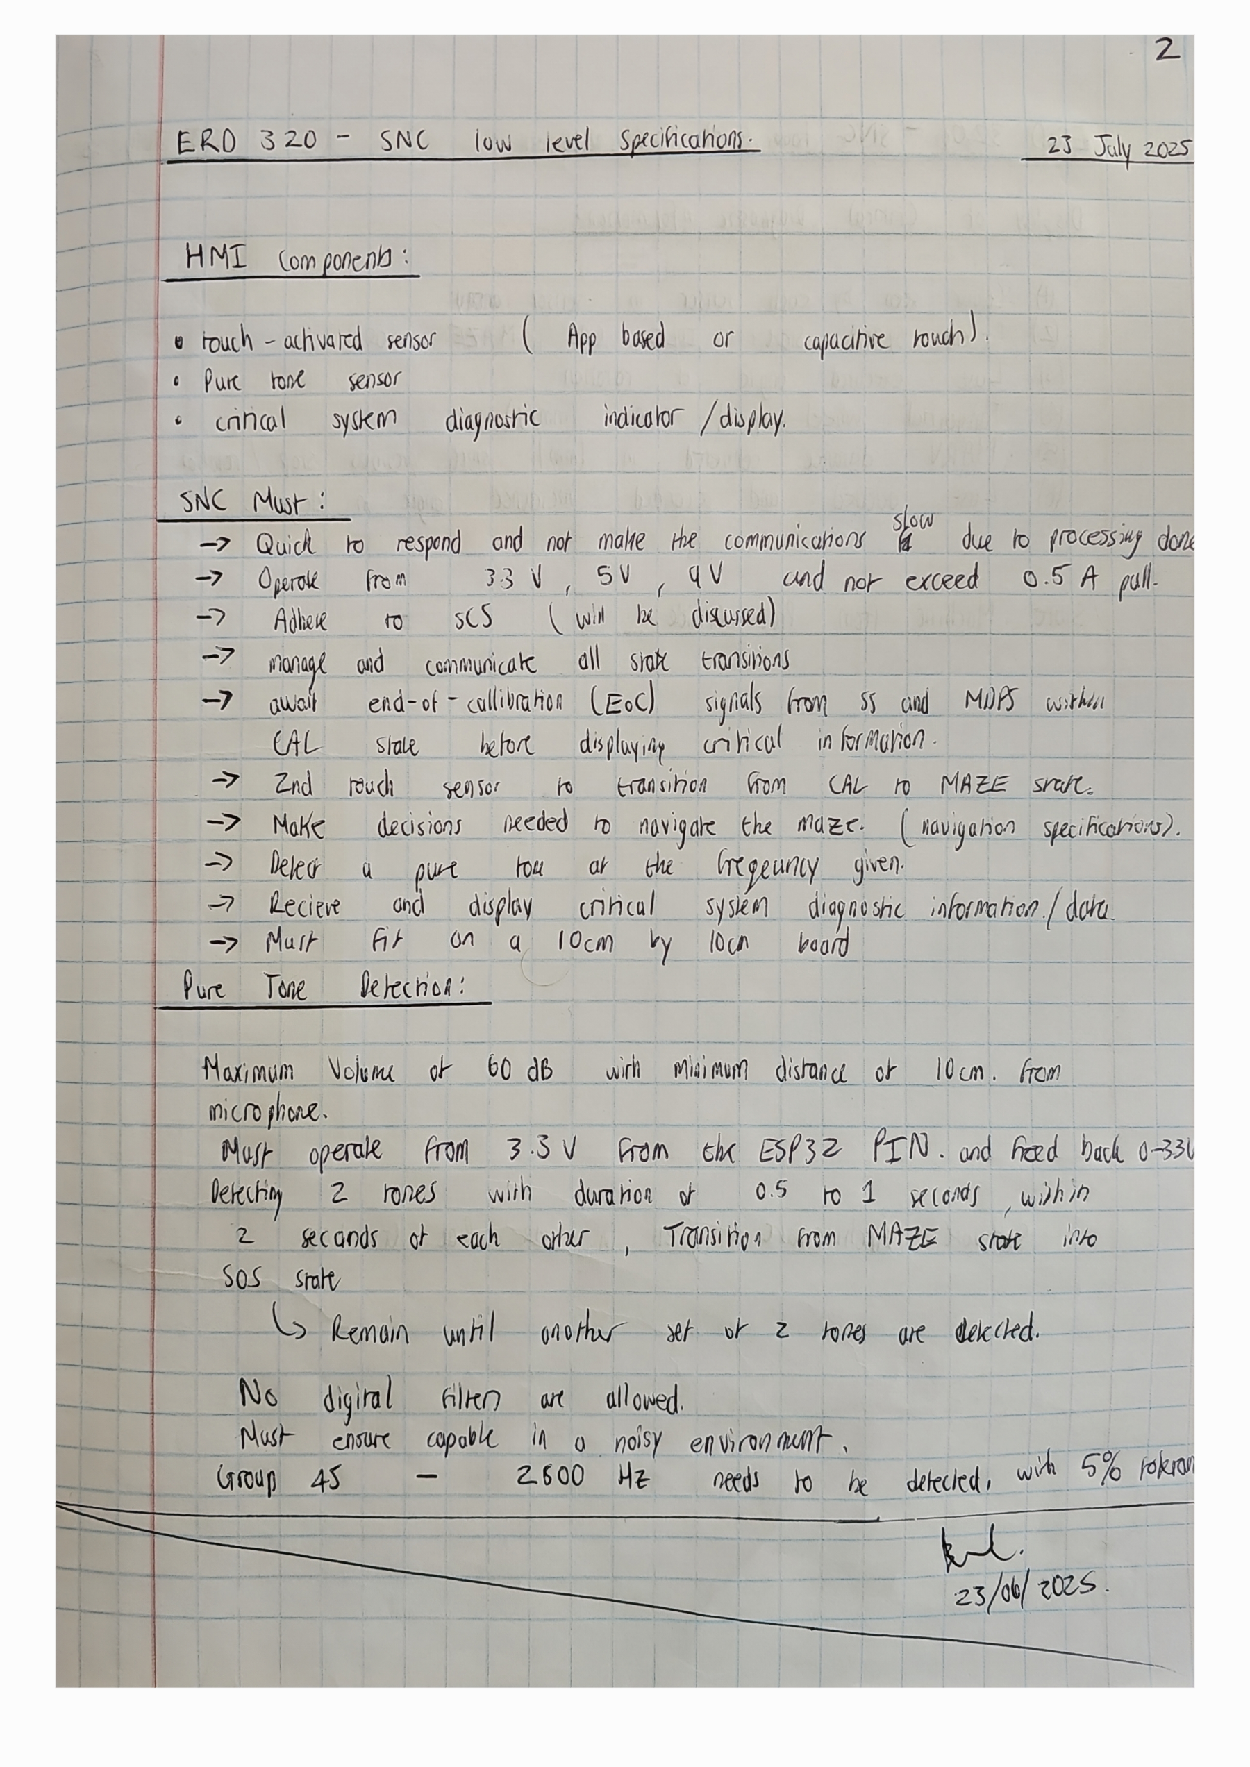
\includegraphics[width=0.9\textwidth]{01_SNC/Labbook/labbook_constraints.pdf}
\caption{Lab book excerpt: Design Constraints analysis for SNC subsystem}
\label{fig:labbook-constraints}
\end{figure}

\stepcounter{subsubsection}  % Increment the section number manually
\subsubsection*{\thesubsubsection\hspace{1em} Trade-offs}

% Insert scanned lab book excerpt documenting trade-off analyses including:
% - Filter order vs. circuit complexity (2nd vs. 4th order decision)
% - Microphone sensitivity vs. noise floor trade-off
% - Envelope time constant vs. responsiveness
% - Comparator threshold setting analysis

\begin{figure}[H]
\centering
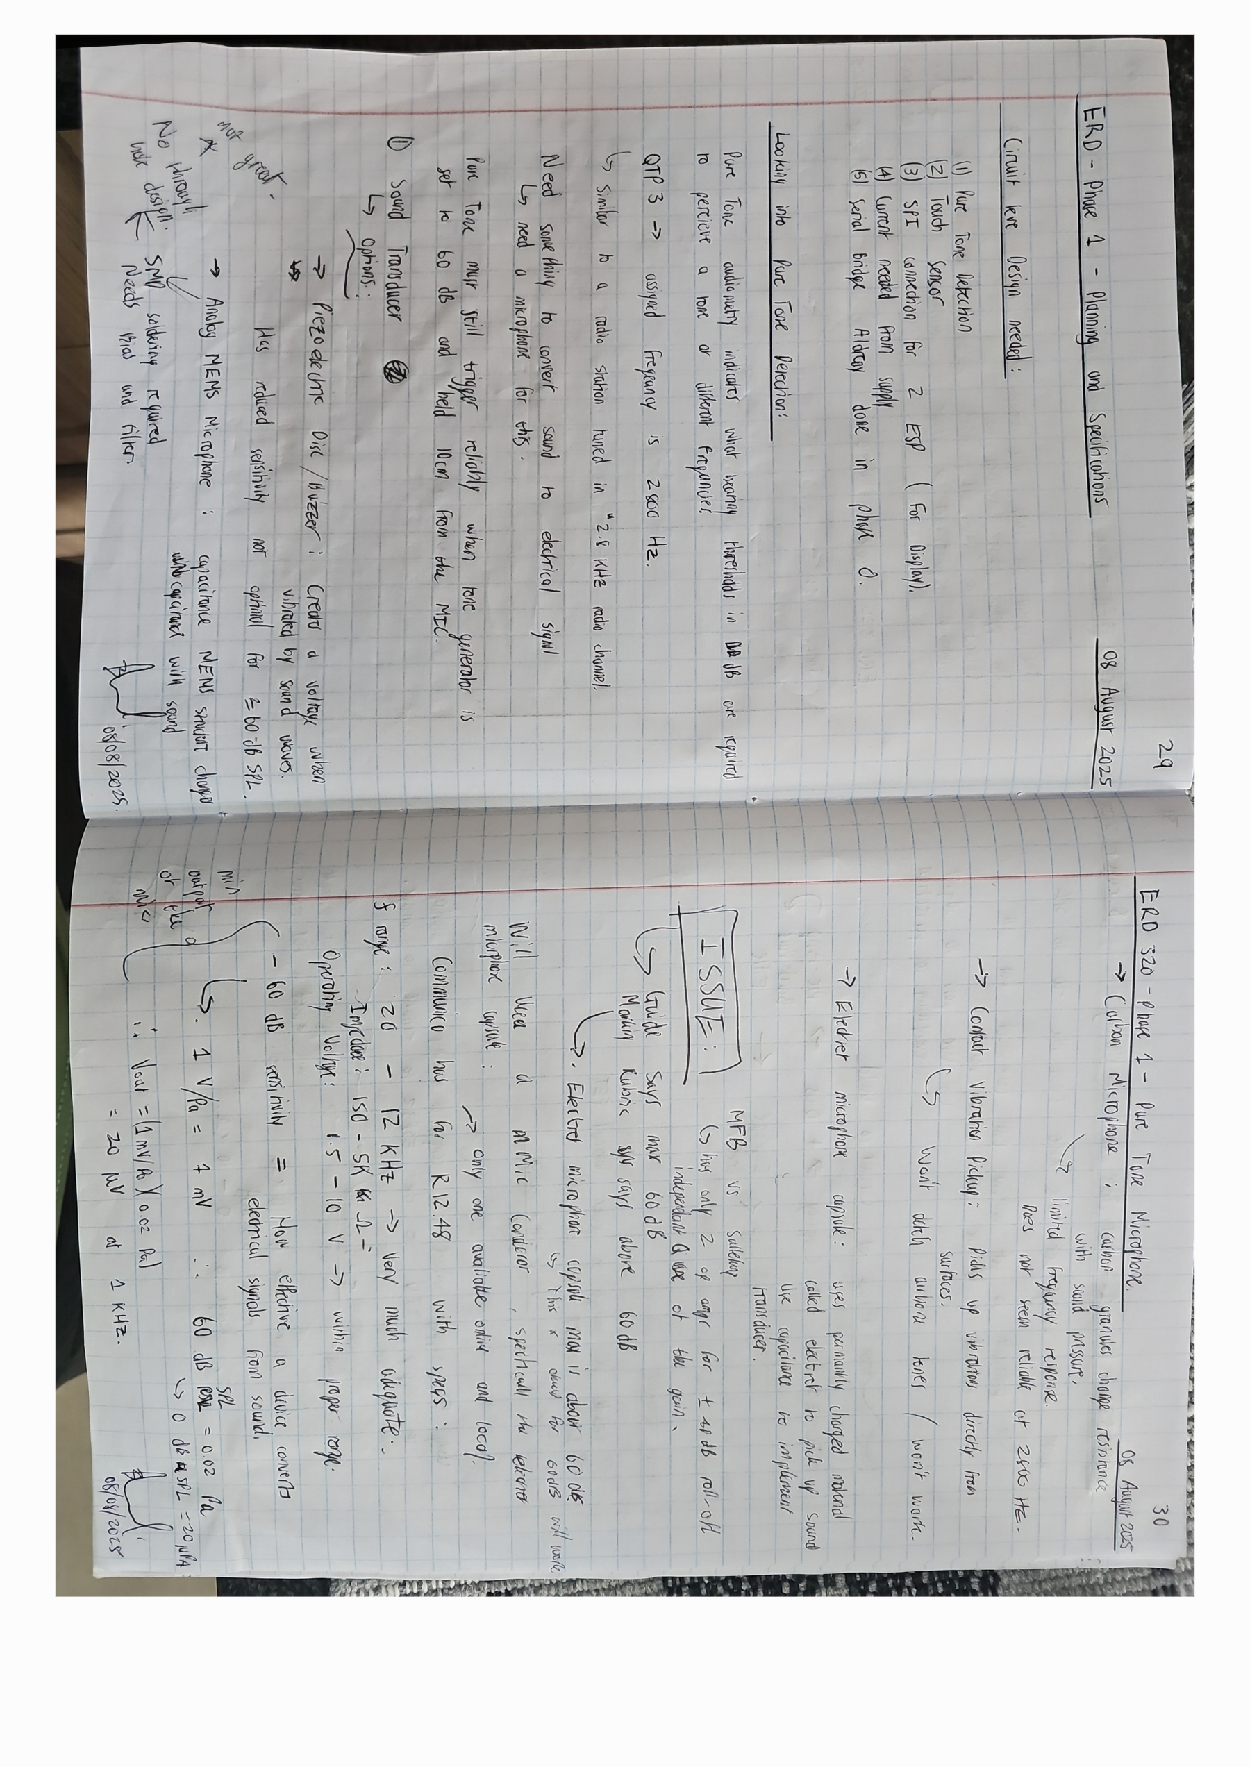
\includegraphics[width=0.9\textwidth]{01_SNC/Labbook/labbook_tradeoffs.pdf}
\caption{Lab book excerpt: Trade-offs analysis for pure tone detection circuit}
\label{fig:labbook-tradeoffs}
\end{figure}

\stepcounter{subsubsection}  % Increment the section number manually
\subsubsection*{\thesubsubsection\hspace{1em} Engineering tools}

% Insert scanned lab book excerpt listing engineering tools used:
% - LTspice XVII for analogue circuit simulation
% - Arduino IDE / PlatformIO for ESP32 firmware development
% - Logic analyzer for protocol timing verification
% - Oscilloscope for analogue signal chain measurement
% - Function generator for tone testing
% - Browser DevTools for web dashboard development

\begin{figure}[H]
\centering
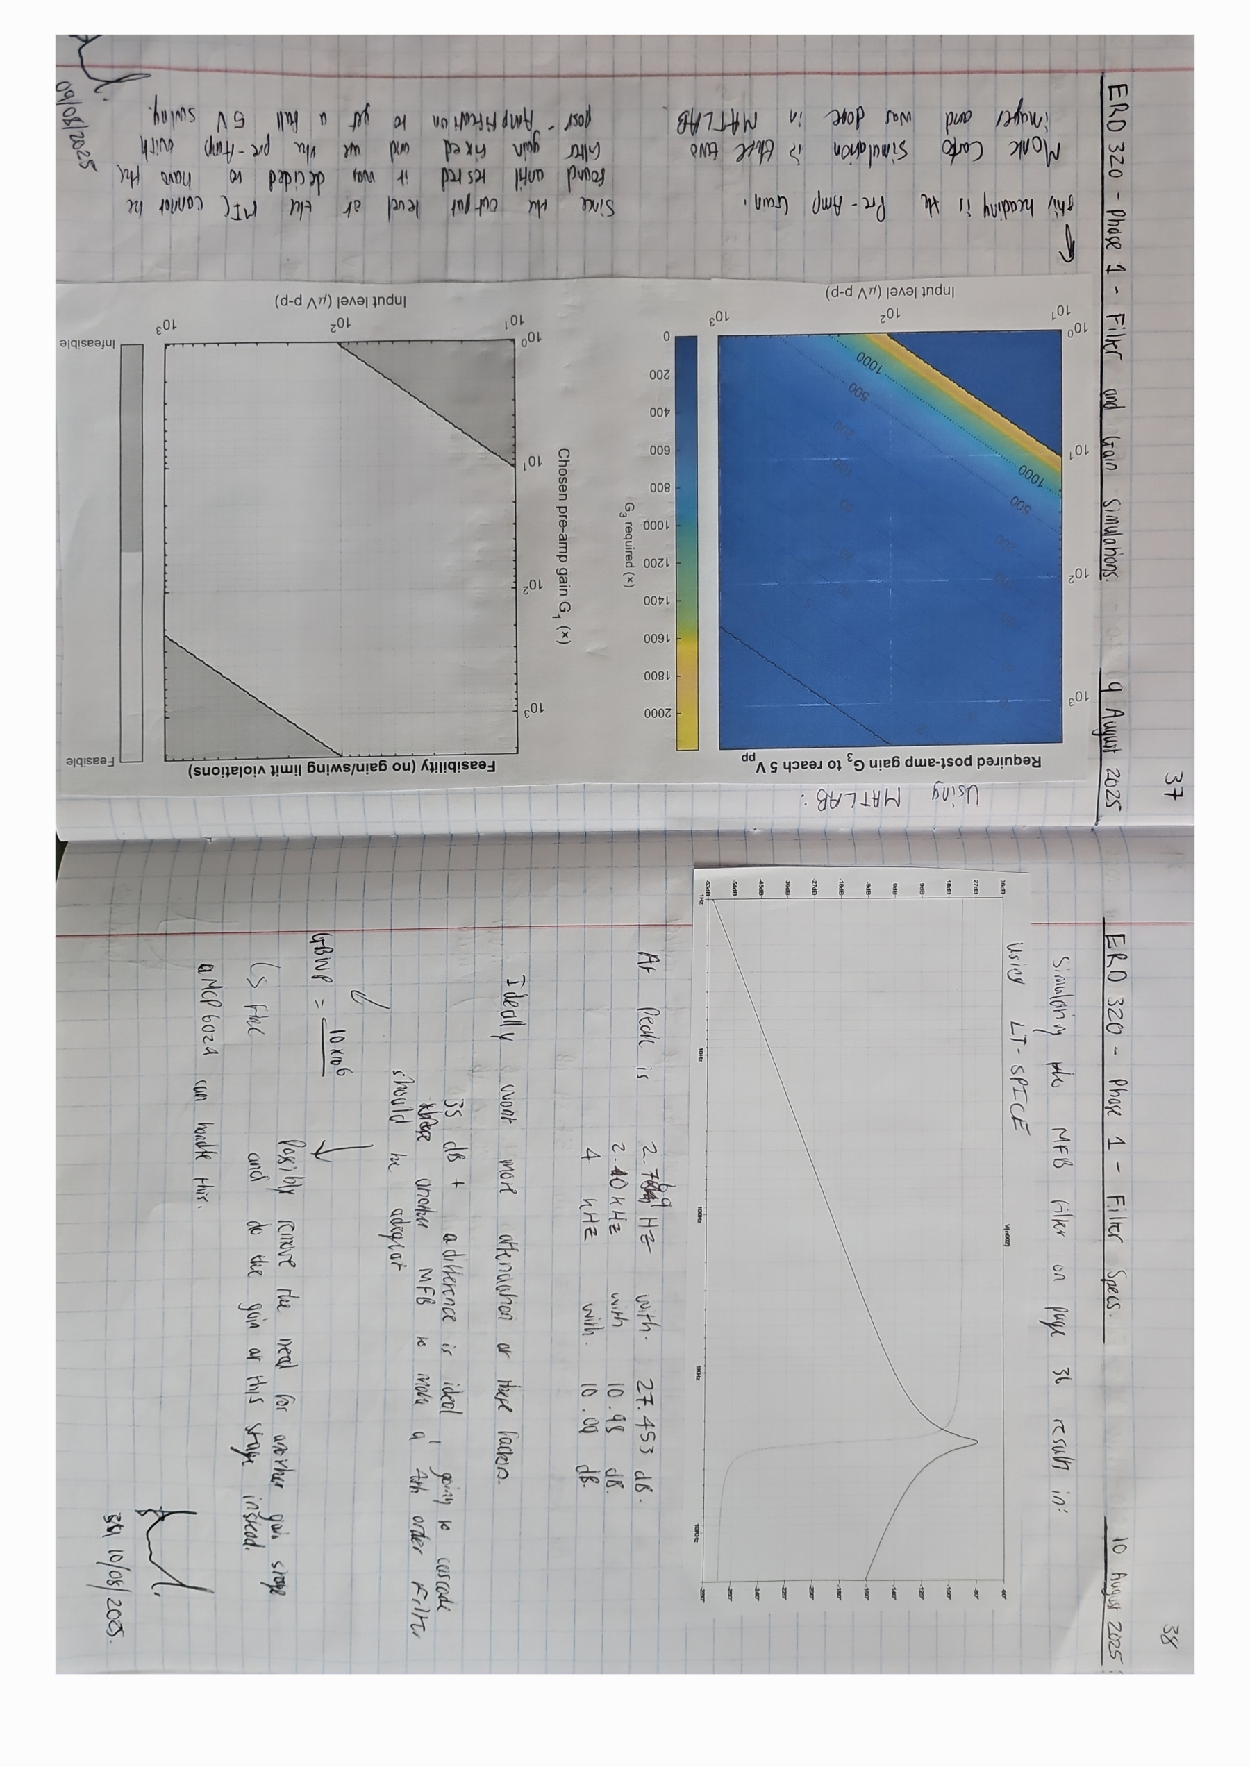
\includegraphics[width=0.9\textwidth]{01_SNC/Labbook/labbook_tools.pdf}
\caption{Lab book excerpt: Engineering tools and test equipment used}
\label{fig:labbook-tools}
\end{figure}

\stepcounter{subsubsection}  % Increment the section number manually
\subsubsection*{\thesubsubsection\hspace{1em} Engineering methods}

% Insert scanned lab book excerpt describing engineering methods:
% - Phase 0 waterfall approach for pure tone detection validation
% - Phase 1-3 iterative/agile firmware development sprints
% - Parameter sweep methodology for filter optimisation
% - Test-driven integration approach (unit → interface → subsystem → full system)

\begin{figure}[H]
\centering
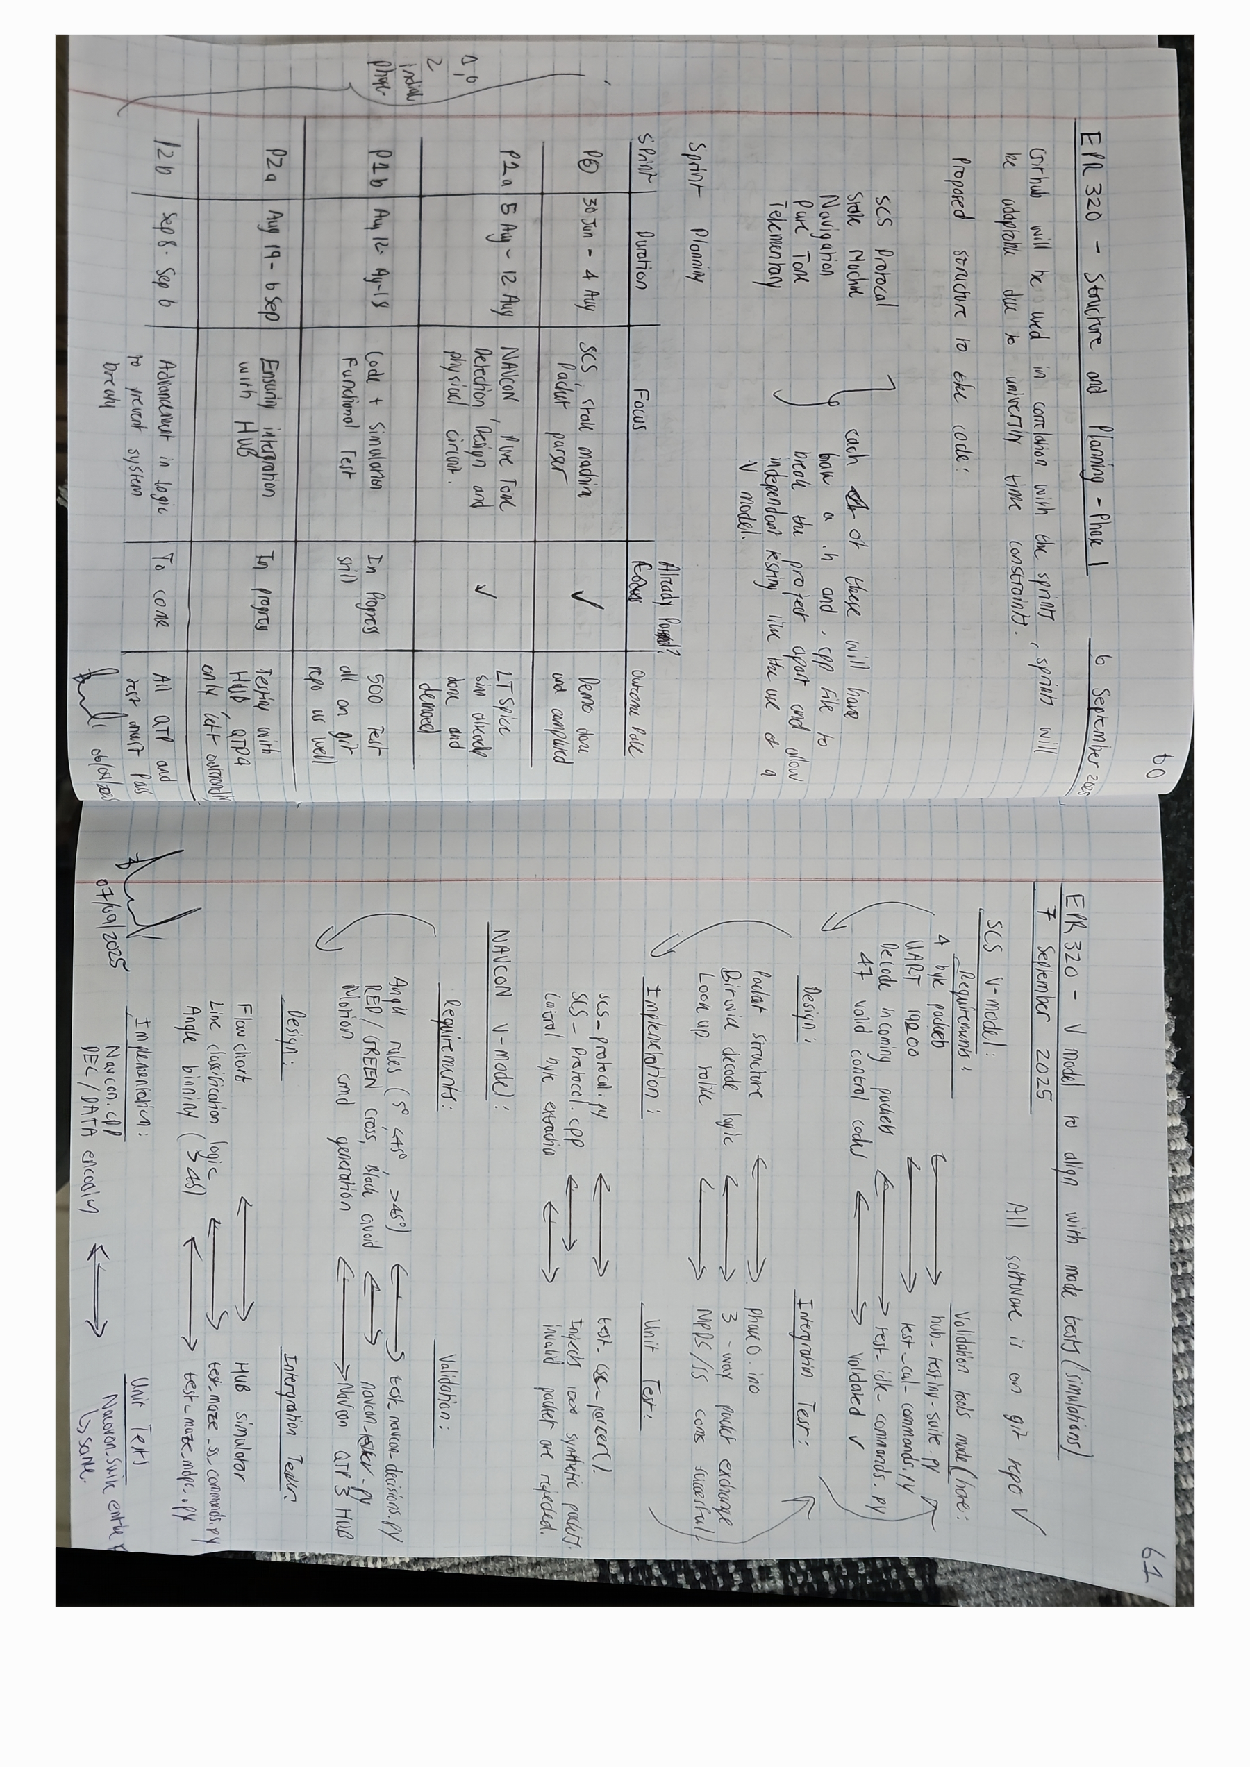
\includegraphics[width=0.9\textwidth]{01_SNC/Labbook/labbook_methods.pdf}
\caption{Lab book excerpt: Engineering methods and development process}
\label{fig:labbook-methods}
\end{figure}

\stepcounter{subsubsection}  % Increment the section number manually
\subsubsection*{\thesubsubsection\hspace{1em} Statements of requirements}

% Insert scanned lab book excerpt with requirements specification:
% - PTD-R-01 through PTD-R-07 (pure tone detection requirements)
% - State machine transition requirements
% - SCS protocol compliance requirements
% - NAVCON functional requirements
% - WiFi telemetry and HMI requirements

\begin{figure}[H]
\centering
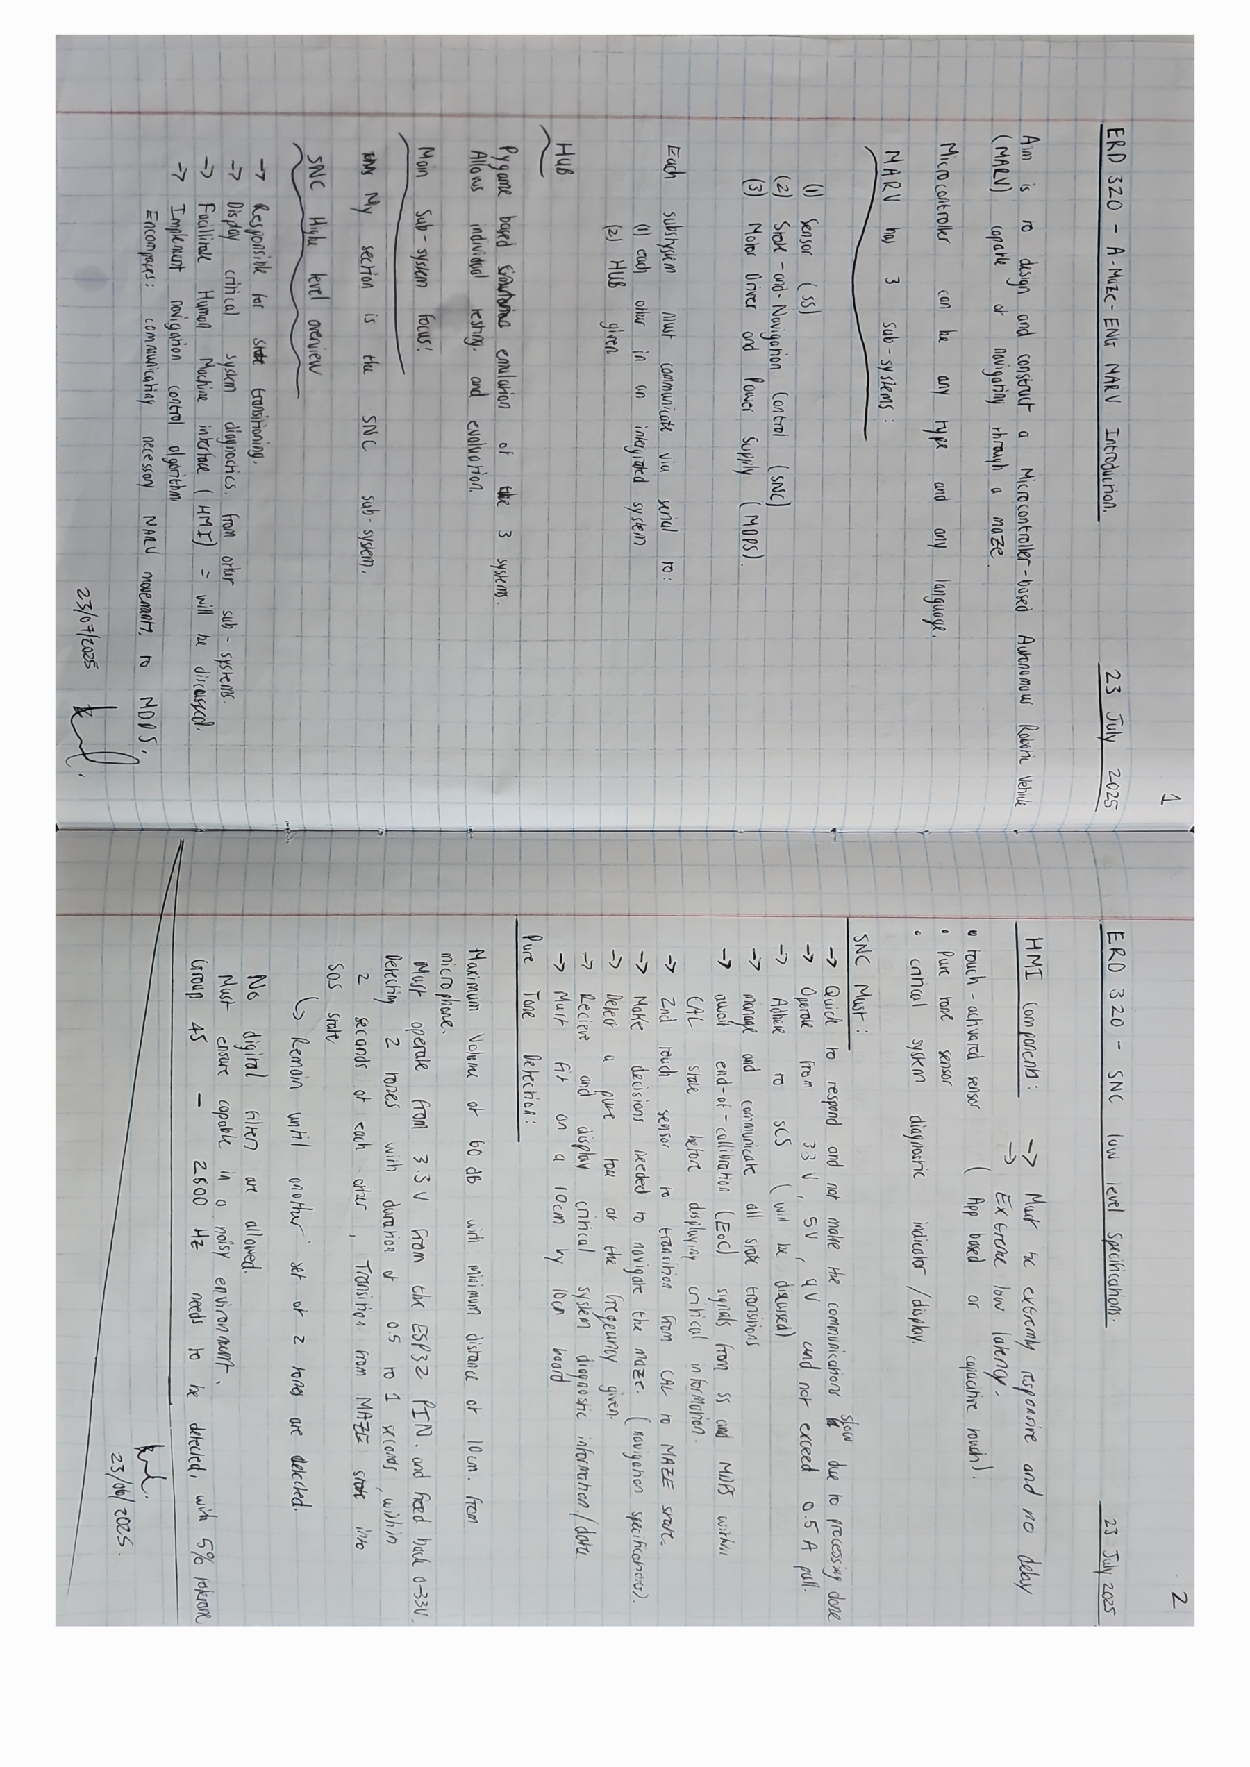
\includegraphics[width=0.9\textwidth]{01_SNC/Labbook/labbook_requirements.pdf}
\caption{Lab book excerpt: Requirements specification for SNC subsystem}
\label{fig:labbook-requirements}
\end{figure}

\stepcounter{subsubsection}  % Increment the section number manually
\subsubsection*{\thesubsubsection\hspace{1em} Development}

% Insert scanned lab book excerpt documenting development activities:
% - Circuit schematic sketches (microphone biasing, \gls{mfb} filter stages, envelope detector)
% - Component value calculations with design equations
% - Breadboard prototype photos/sketches
% - Initial testing observations and issues encountered
% - Iterative design refinements

\begin{figure}[H]
\centering
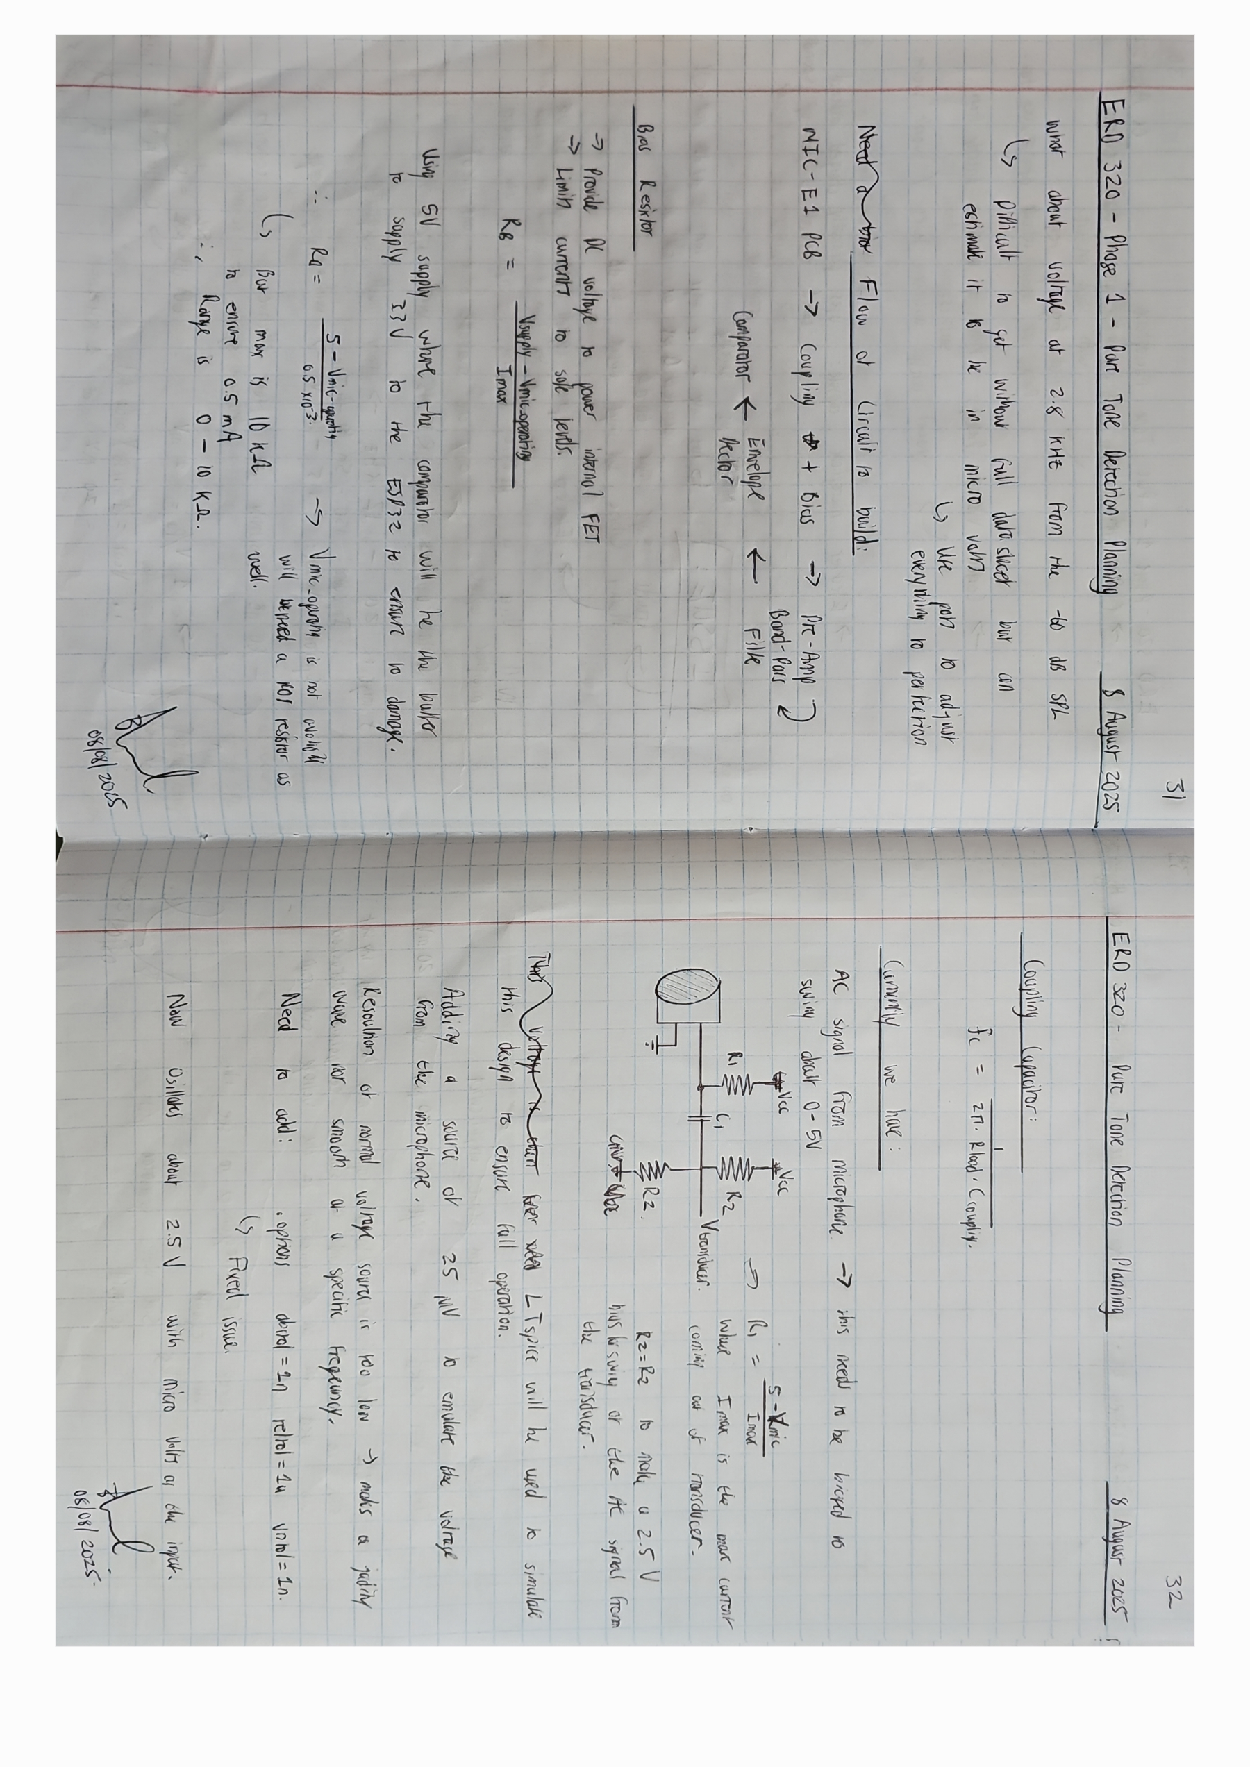
\includegraphics[width=0.9\textwidth]{01_SNC/Labbook/labbook_development.pdf}
\caption{Lab book excerpt: Development activities and circuit prototyping}
\label{fig:labbook-development}
\end{figure}

\stepcounter{subsubsection}  % Increment the section number manually
\subsubsection*{\thesubsubsection\hspace{1em} Simulations}

% Insert scanned lab book excerpt showing simulation results:
% - LTspice frequency response plots (Bode plots showing 2800 Hz passband)
% - Transient simulation of envelope detector with 2800 Hz input
% - Q-factor and bandwidth calculations from simulation data
% - Component tolerance sensitivity analysis results
% - Comparator threshold crossing timing

\begin{figure}[H]
\centering
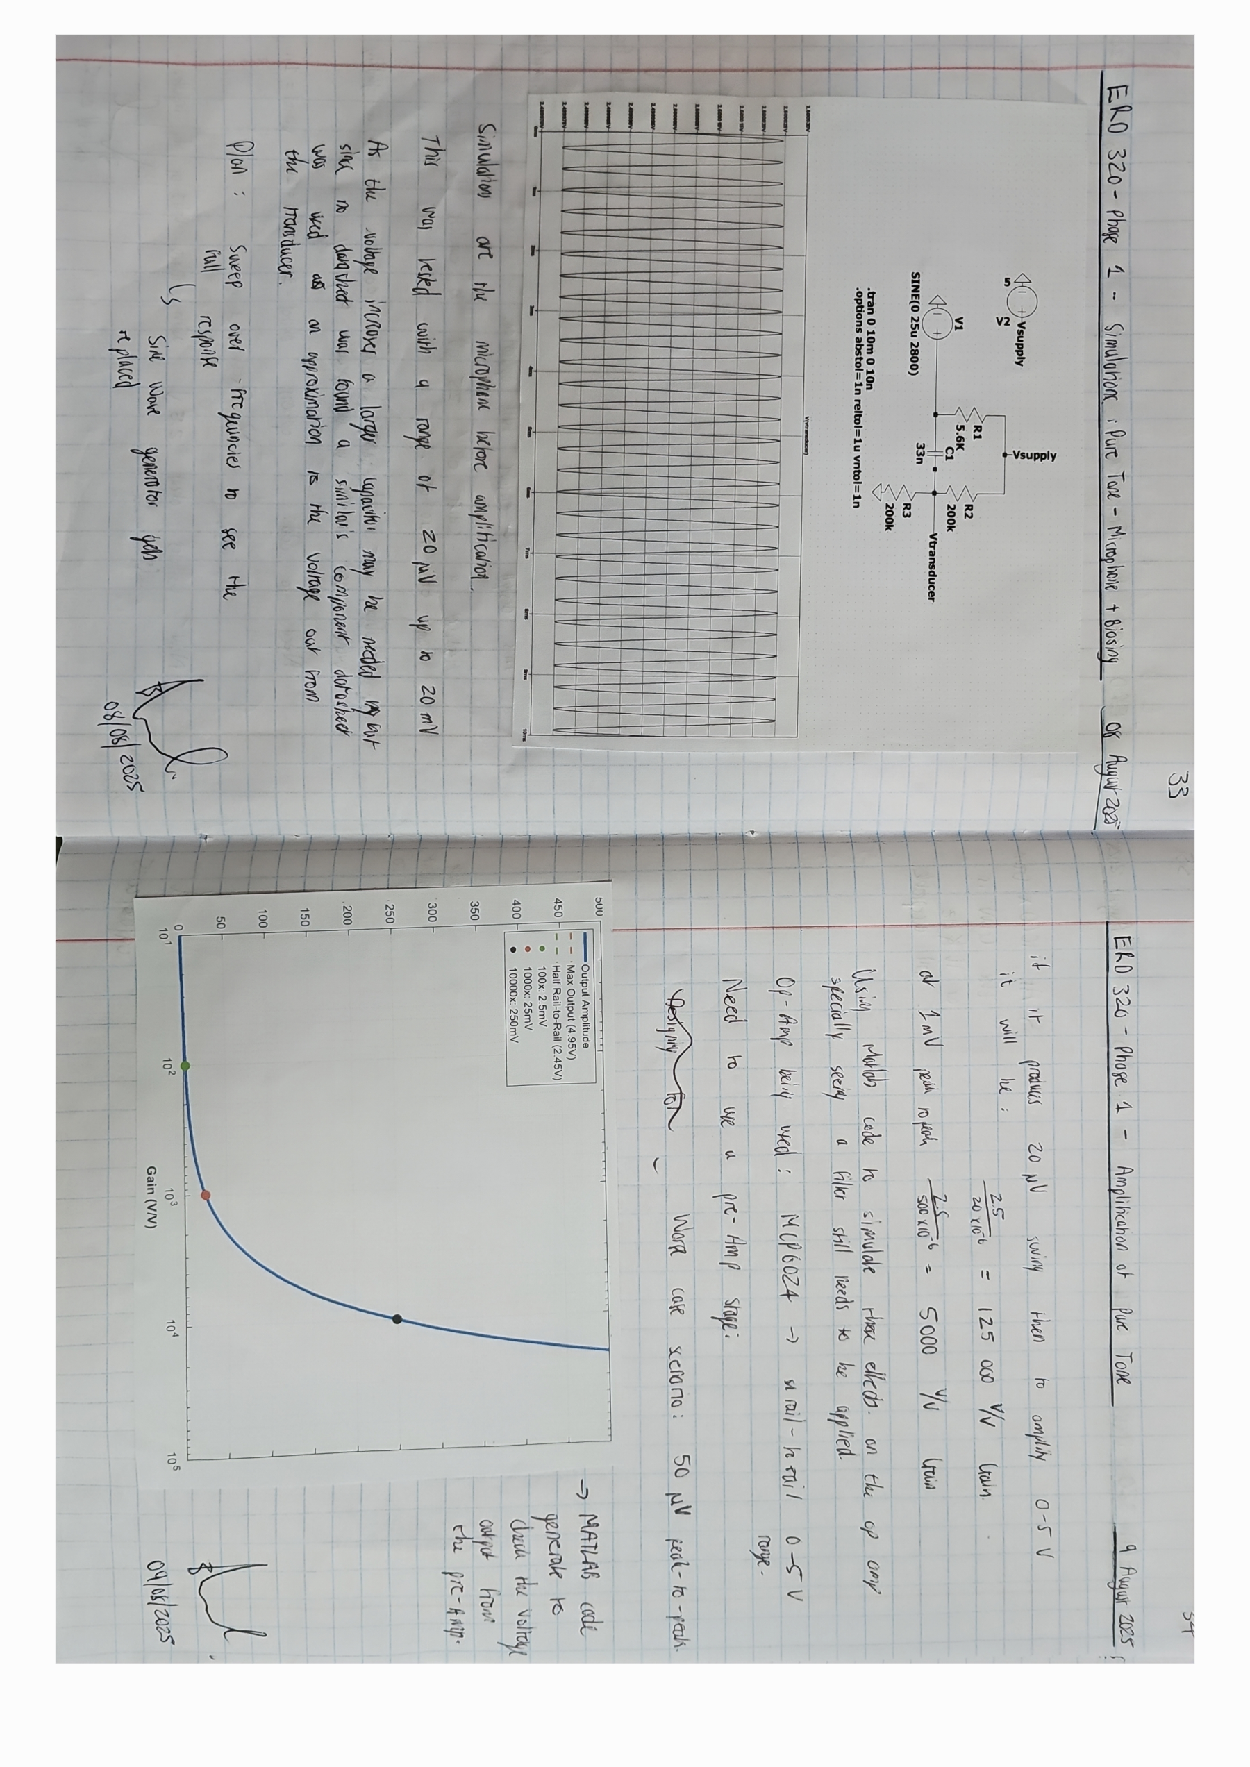
\includegraphics[width=0.9\textwidth]{01_SNC/Labbook/labbook_simulations.pdf}
\caption{Lab book excerpt: SPICE simulation results and analysis}
\label{fig:labbook-simulations}
\end{figure}

\stepcounter{subsubsection}  % Increment the section number manually
\subsubsection*{\thesubsubsection\hspace{1em} Approach to coding and testing}

% Insert scanned lab book excerpt describing firmware development approach:
% - State machine implementation strategy (IDLE/CAL/MAZE/SOS)
% - NAVCON decision logic structure and rule hierarchy
% - SCS protocol parser implementation notes
% - Unit testing approach for packet validation
% - Integration testing with HUB simulator
% - Debugging strategies and tools (serial monitor, logic analyzer traces)

\begin{figure}[H]
\centering
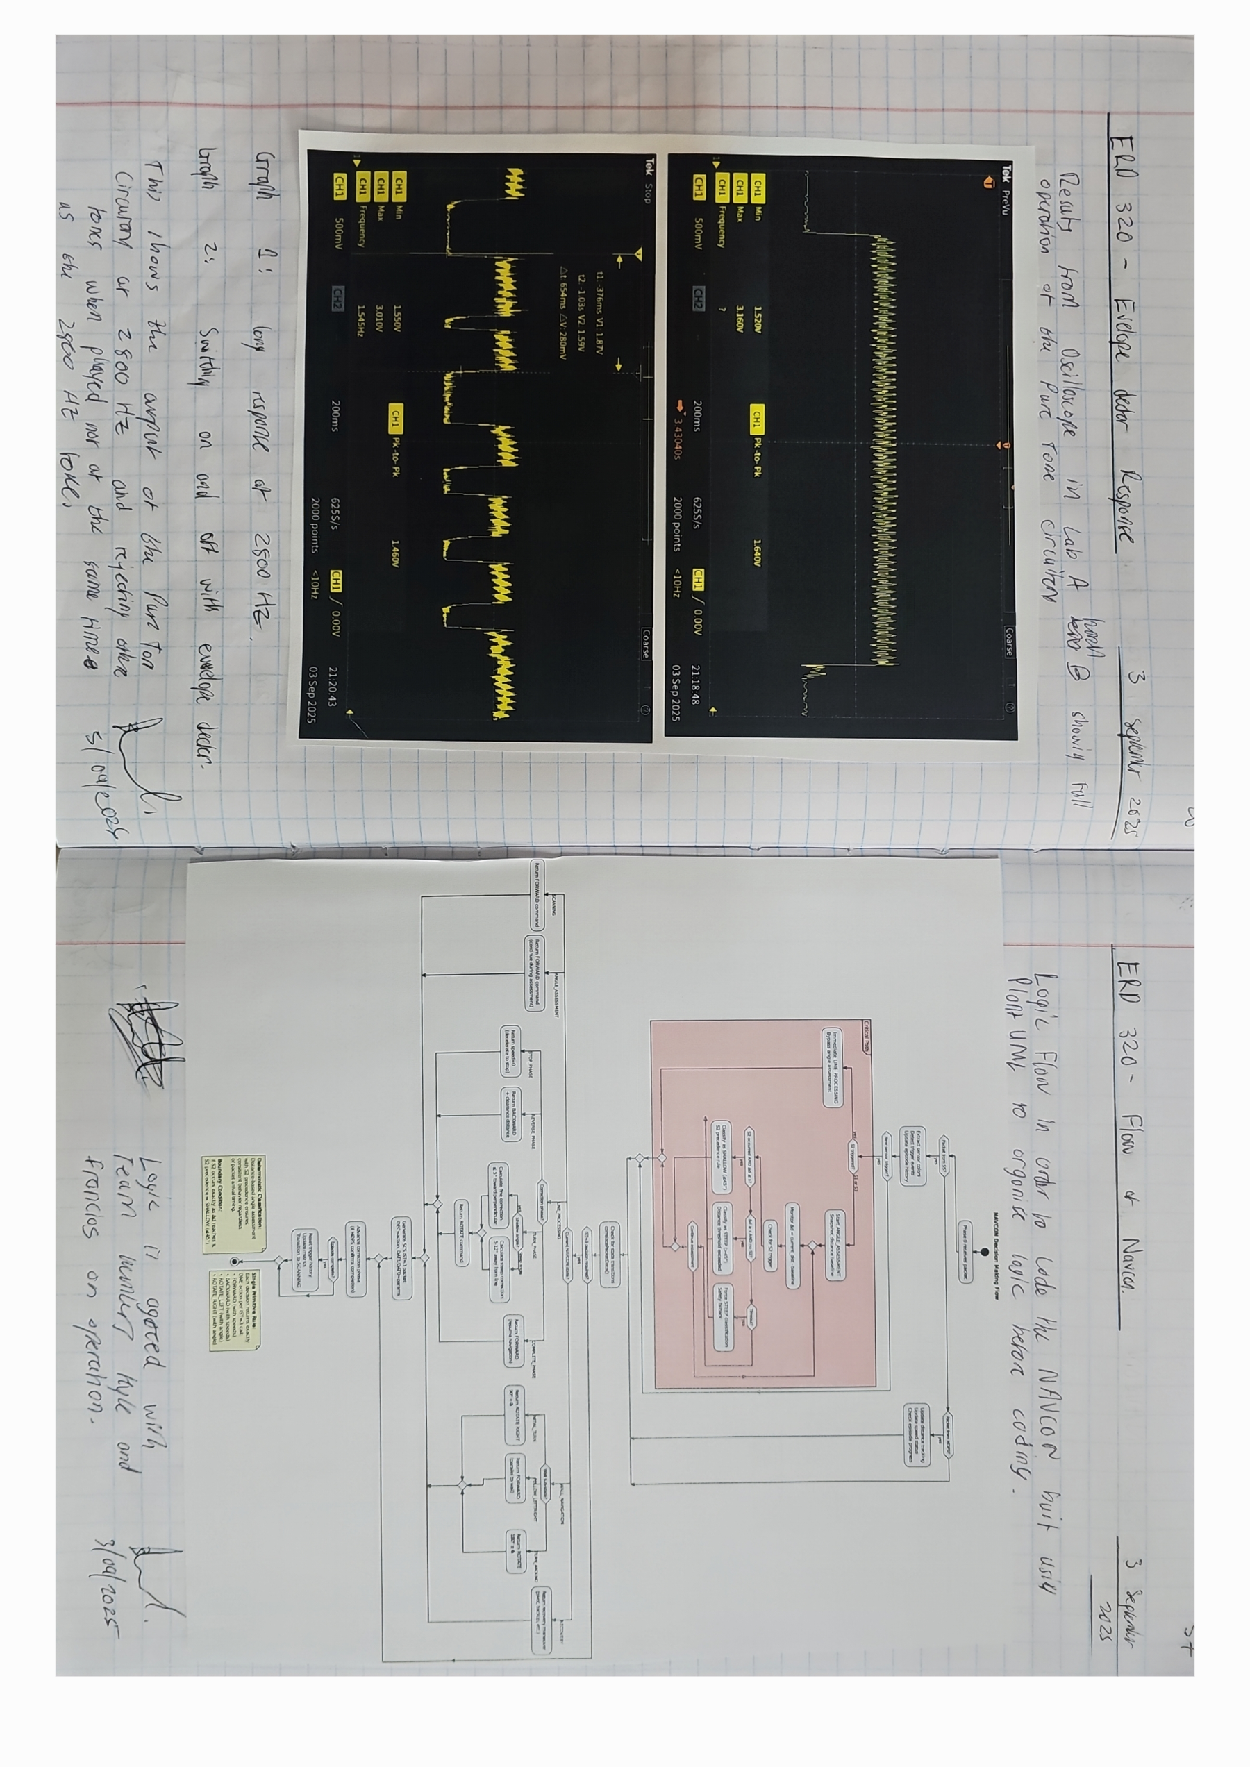
\includegraphics[width=0.9\textwidth]{01_SNC/Labbook/labbook_coding.pdf}
\caption{Lab book excerpt: Approach to firmware coding and testing}
\label{fig:labbook-coding-testing}
\end{figure}



\newpage

% ============================================================================
% SUBSYSTEM 2
% ============================================================================
\section{Subsystem 2}
%\textit{Maximum 20 pages per subsystem (excluding lab book excerpts).}

%\subsection{Title: SNC Subsystem}

\textbf{Subsystem Name:} State-and-Navigation Control (SNC) Subsystem

\textbf{Student Name:} Byron Norval

\textbf{Student Number:} u21444758

\subsection{Subsystem Needs Analysis}


% Write your subsystem needs analysis here
A crucial element of the autonomous vehicle known as MARV is the SS(sensor subsystem). In this context, one that is capable of navigating a maze for which the only guides to the end are coloured lines, representing different obstacles on a PVC mat.

The MARV will need to identify the obstacles by interpreting the colour of the lines on the maze. This means that SS will need some form of colour detection.

To prevent the disturbance of changing ambient light, SS will need to minimise its influence when performing colour detection.

The MARV will need to keep track of the MARVs orientation inside the maze. This means that SS will need to calculate the angle of incidence when crossing the lines. 

SS will need to integrate with the full system with minimal change in functionality and operation.

For SS to integrate with the full system, SS will need to use the communication protocol provided, which will enable seamless communication with other subsystems.

Though SS is a subsystem, it needs to work independently as well for testing during development. This means that SS will need its own power supply. 

The afore mentioned needs for SS are shown in a context diagram to better illustrate the subsystem's place in the system as a whole.


\begin{figure}[H]
\centering
\includegraphics[width=0.9\textwidth]{02_SS/figures/context_diagram.png}
\caption{Context Diagram For The SS(Sensor Subsystem)}
\label{fig:pure-tone-detection-flow}
\end{figure}


\subsection{Subsystem Concept Exploration}
\textit{-	Refer to Kossiakoff, Chapter 6, 7 and 8\\
-	Do a brief survey of literature on possible methods / circuits / designs that could meet the above needs, other than the prescribed subsystem. MAKE SURE THAT THE DOCUMENTS YOU REFERENCE ARE INCLUDED IN SECTION 1.2!!!}

% Write your concept exploration here

\subsubsection{Colour Detection Sensors}

\subsubsection{Incidence Angle Detection}
%======================================================================
\subsection{SNC Subsystem Concept Definition}
\label{subsec:snc-concept-definition}
%======================================================================

The \gls{snc} subsystem implements centralized coordination, navigation decision-making, and operator interaction for the \gls{marv} platform. The design employs hierarchical state-machine architecture with separation of concerns. State management is decoupled from navigation logic. The design implements deterministic transitions, \gls{hub} compatibility for testability, \gls{sos} override capability, and \gls{scs} protocol compliance.

%----------------------------------------------------------------------
\subsubsection{Operational Concept}

System operation follows a four-state sequence: IDLE initialization, CAL calibration with dual \gls{eoc} assertion, MAZE autonomous navigation with \gls{navcon} logic, and \gls{sos} operator safety override via 2800~Hz dual-tone detection. Touch activation triggers IDLE$\rightarrow$CAL, dual \gls{eoc} enables CAL$\rightarrow$MAZE, \gls{eom} returns MAZE$\rightarrow$IDLE, and dual-tone toggles MAZE$\leftrightarrow$\gls{sos}.

\begin{figure}[H]
\centering
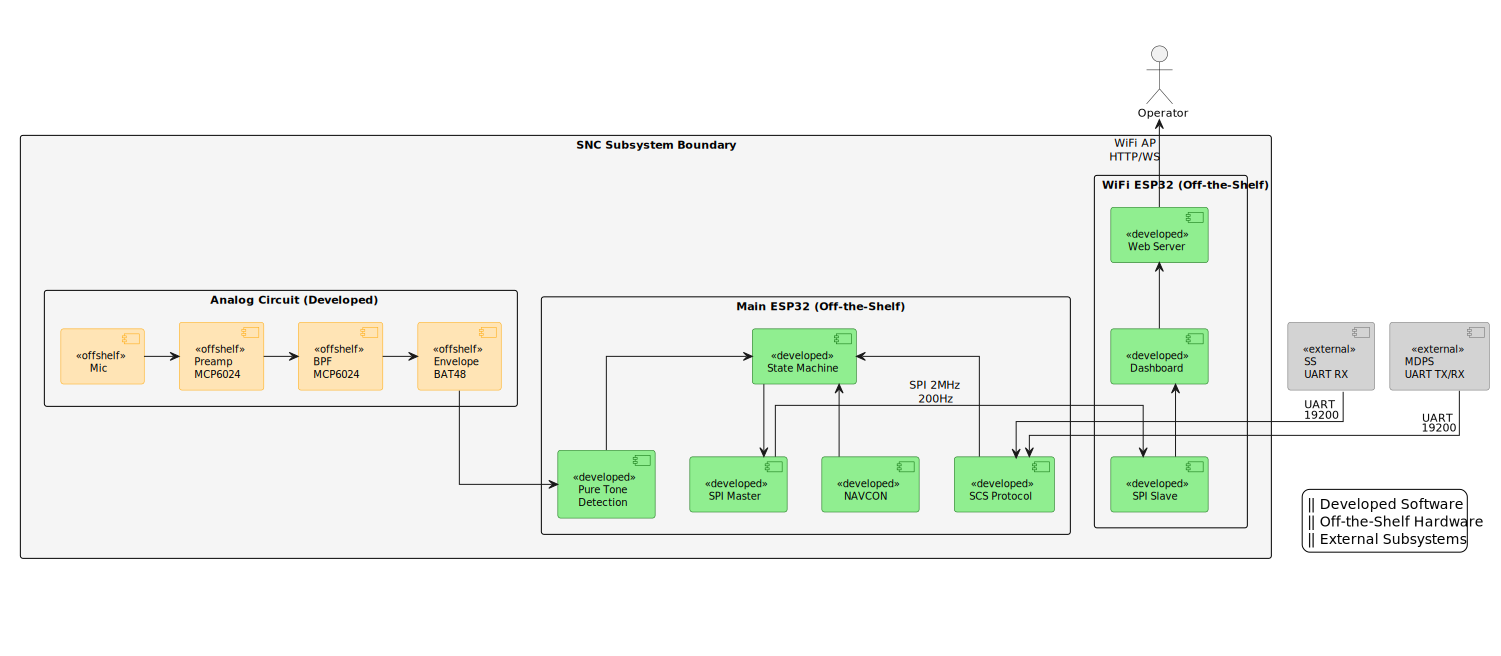
\includegraphics[width=1.05\textwidth]{01_SNC/diagrams/snc_architecture/out/snc_architecture.pdf}
\caption{\gls{snc} Architecture showing hardware and software with developed components in green, off-the-shelf in orange. Main ESP32 executes control, WiFi ESP32 handles telemetry, analogue circuit detects tones.}
\label{fig:snc-architecture-hw-sw}
\end{figure}

%----------------------------------------------------------------------
\subsubsection{Architecture Overview}

Figure~\ref{fig:snc-architecture} presents the \gls{snc} subsystem functional block diagram showing layered architecture with component interactions and data flows.

\begin{figure}[H]
\centering
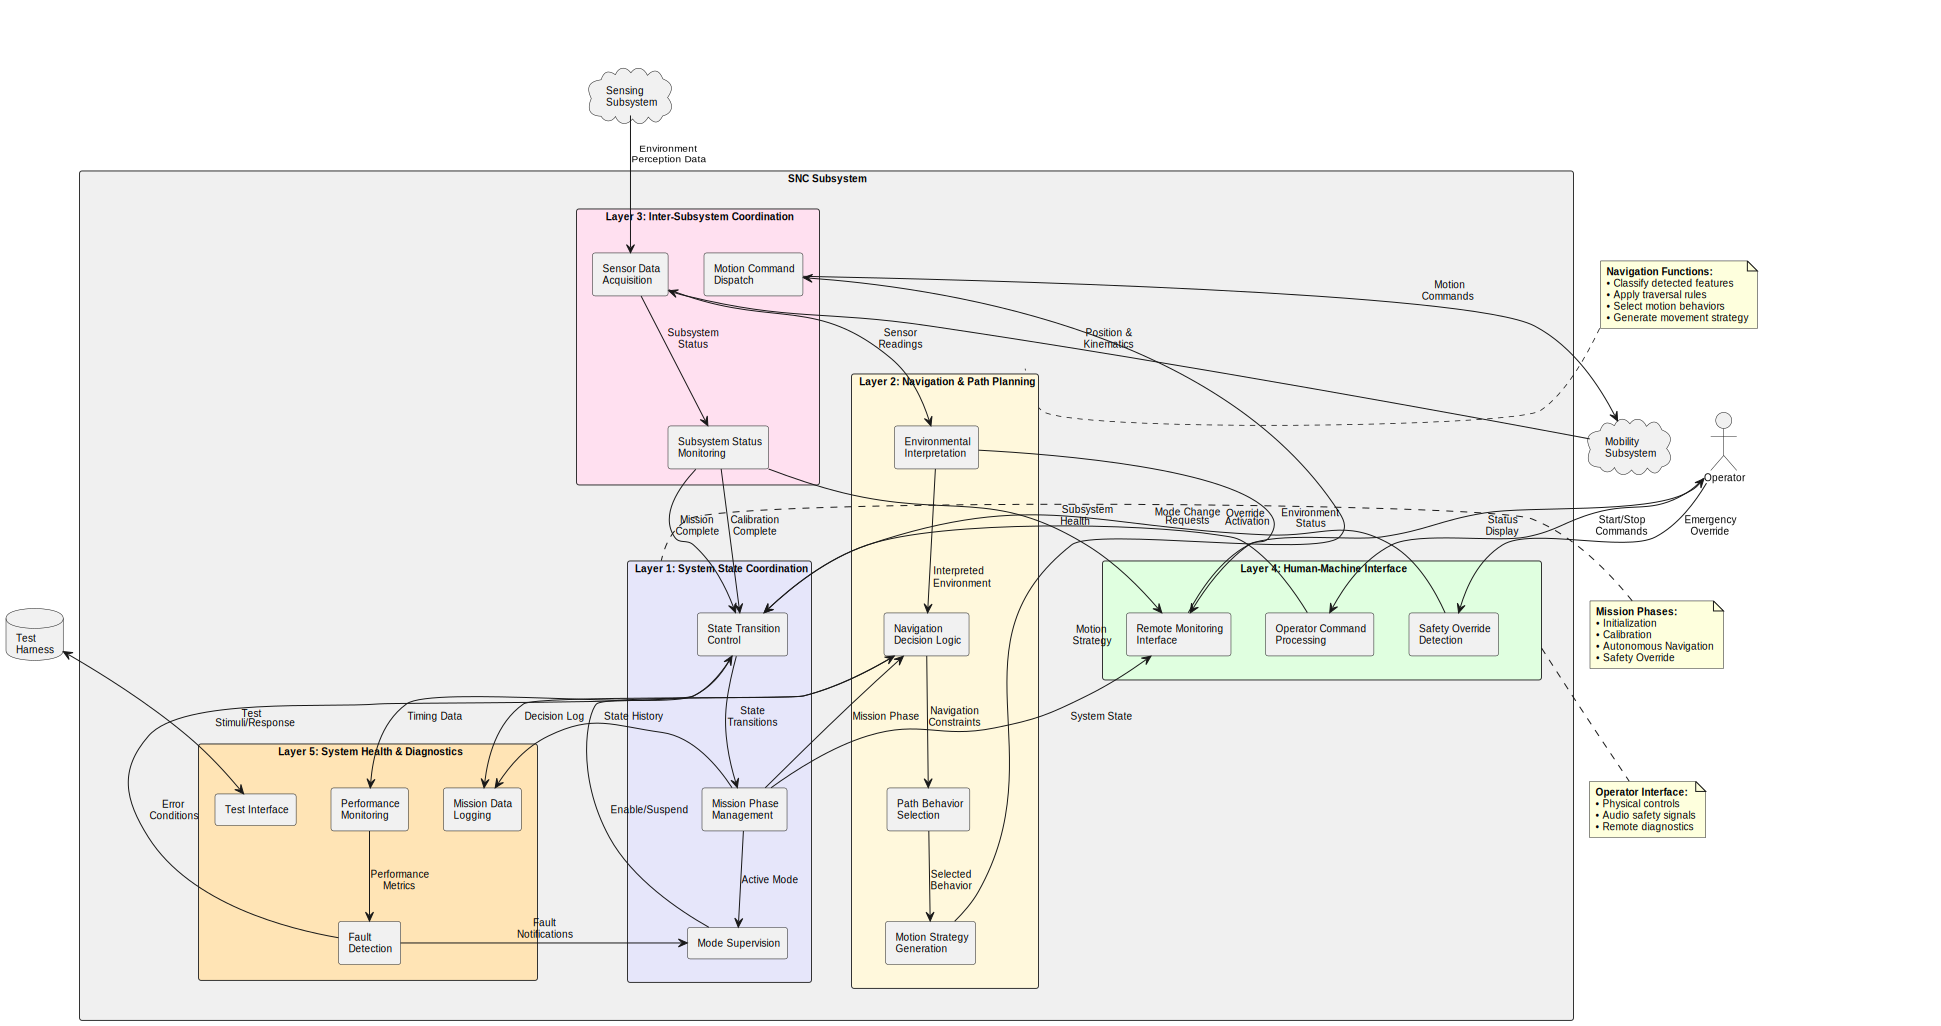
\includegraphics[width=0.98\textwidth]{01_SNC/diagrams/architecture_block/out/architecture_block.pdf}
\caption{\gls{snc} Subsystem Functional Block Diagram showing layered architecture: State Management, Navigation Decision, Communication Protocol, Touch/Tone Input, and Supervision \& Diagnostics.}
\label{fig:snc-architecture}
\end{figure}

The hardware comprises Main ESP32 managing state machine, \gls{navcon}, \gls{scs} protocol, touch sensor, and tone GPIO. WiFi ESP32 handles web server, telemetry dashboard, and \gls{spi} slave interface. The Pure Tone Circuit includes microphone, preamplifier, 4th-order 2800~Hz bandpass filter, envelope detector, and comparator. Capacitive Touch uses ESP32 TOUCH pin with 50~ms debouncing.

Software components include the State Machine implementing IDLE, CAL, MAZE, and \gls{sos} with guard conditions. NAVCON Logic applies angle-dependent navigation rules. The SCS Protocol Stack operates at UART 19200 baud with 4-byte packets. SPI Telemetry transmits at 200~Hz to WiFi ESP32 using 257-byte packets with DMA. The Web Dashboard uses HTML5 and JavaScript interface for real-time diagnostics.

External interfaces connect via UART at 19200 baud to \gls{ss} for RX and \gls{mdps} for TX and RX per \gls{scs} specification. Internal \gls{spi} at 2~MHz links Main and WiFi ESP32 with 200~Hz telemetry. WiFi AP operates at 192.168.4.1 with HTTP server on port 80 and WebSocket on port 81. Capacitive touch and tone circuit GPIO connect to Main ESP32.

%======================================================================

\subsection{Subsystem Engineering Design}
\label{subsec:snc-engineering-design}

\subsubsection{Design Constraints and Trade-offs}

\paragraph{Design Constraints}

Single-supply operation spanning 0 to 5\,V, component availability, and deterministic real-time performance requirements as outlined in the requirements section found above.

\paragraph{Key Trade-offs}

Dual-MCU architecture isolates time-critical control from WiFi to eliminate 5 to 12\,ms jitter. 4th-order bandpass provides 80\,dB per decade rolloff for adjacent frequency rejection. Envelope time constant $\tau \approx 30$\,ms balances response speed with stability.

\subsubsection{Development Methodology}

\paragraph{Tools}

LTspice XVII, Arduino IDE 2.3.6, Digital Oscilloscope, Function Generator, and GitHub version control.

\paragraph{Approach}

Hybrid V-model applied for analogue circuit validation. Agile sprints implemented for firmware including \gls{scs}, state machine, \gls{navcon}, and telemetry.

\paragraph{Version Control}

GitHub repository contains 147 commits across 12 branches. Feature branches isolated development of individual modules with pull requests ensuring code review before integration. Tag-based releases marked completion of calibration, maze navigation, and \gls{sos} detection milestones.

\paragraph{Modular Architecture}

Firmware structured into separate .h and .cpp file pairs for independent unit testing before system integration: \texttt{SCS\_Protocol.h} and \texttt{SCS\_Protocol.cpp} for packet handling, \texttt{NAVCON.h} and \texttt{NAVCON.cpp} for navigation logic, \texttt{StateMachine.h} \texttt{StateMachine.cpp} for system state coordination, \texttt{PureTone.h} and \texttt{PureTone.cpp} for dual-tone detection, and \texttt{SPI\_Telemetry.h} and \texttt{SPI\_Telemetry.cpp} for WiFi communication. Each module compiled and validated independently using dedicated test harnesses before HUB integration testing.

\subsubsection{Pure Tone Detection Circuit Design}

The analogue signal chain for 2800~Hz dual-tone detection implements operator-initiated \gls{sos} state activation addressing requirements FN-4, ON-3, and DR-3 with analogue filtering and digital validation.

\paragraph{Architectural Overview}

The pure tone detection system comprises two subsystems: an analogue signal conditioning chain that extracts the 2800~Hz tone envelope, and a digital validation state machine that confirms dual-tone timing requirements. Figure~\ref{fig:pure-tone-detection-flow} presents the full detection flow from acoustic input through analogue signal processing to digital validation and SOS state triggering.

\begin{figure}[H]
\centering
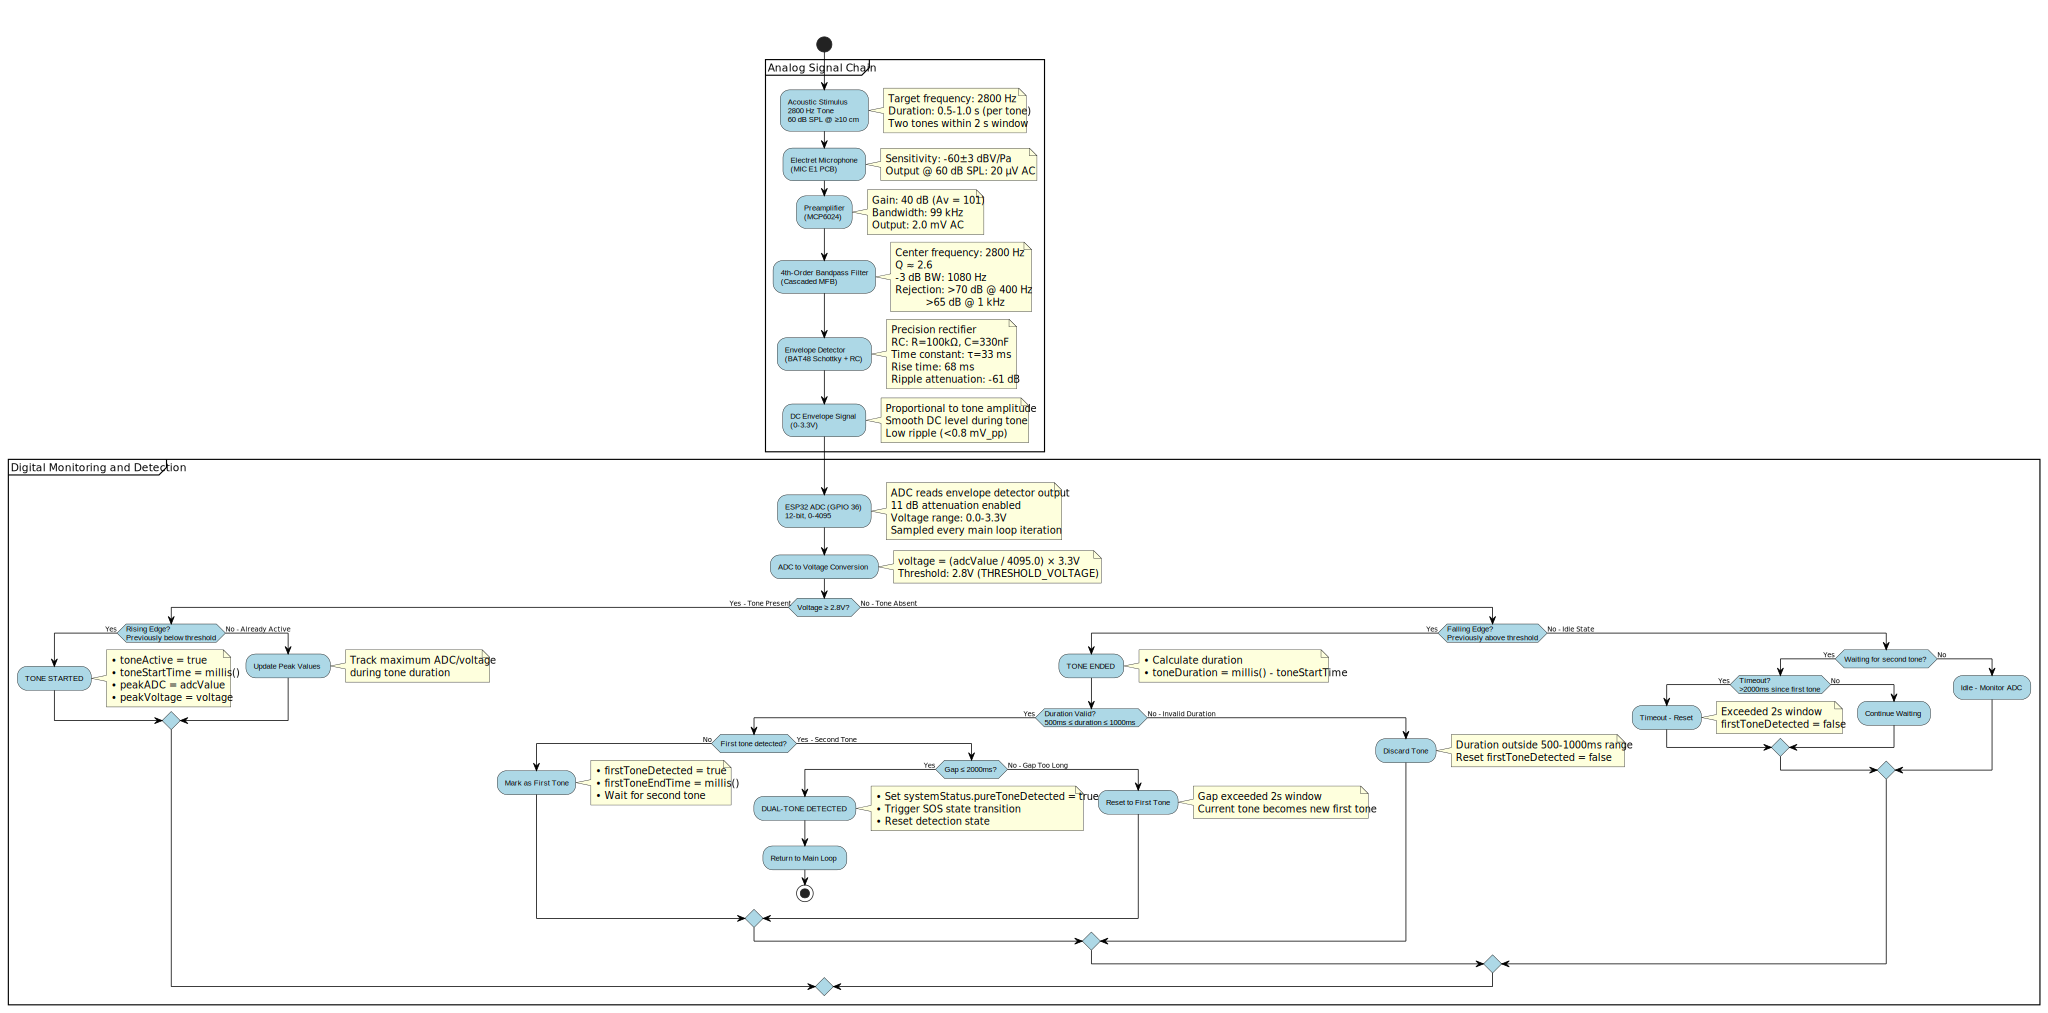
\includegraphics[width=1.05\textwidth]{01_SNC/diagrams/pure_tone_detection_flow/out/pure_tone_detection_flow.pdf}
\caption{Pure Tone Detection Flow: Analog Signal Chain and Digital Validation}
\label{fig:pure-tone-detection-flow}
\end{figure}

\paragraph{Component Selection Rationale}

\subparagraph{MCP6024 Op-Amp}

Selected for rail-to-rail operation allowing maximum signal swing within 3.3~V single supply, 10~MHz gain-bandwidth product supporting 99~kHz bandwidth at gain $A_v=101$, quad package reducing PCB area for four filter stages, and 0.9~mA per amplifier for battery operation.

\subparagraph{BAT48 Schottky Diode}

Low forward voltage $V_F \approx 0.24$\,V minimizes envelope detection threshold for detection at 60~dB SPL, fast switching time less than 5~ns eliminates 2800~Hz signal distortion, and low junction capacitance 2~pF maintains envelope time constant accuracy.

\subparagraph{Dual-MCU Architecture}

Main ESP32 dedicated to deterministic control eliminates 5 to 12~ms WiFi jitter from navigation timing, WiFi ESP32 isolated for non-critical telemetry streaming at 200~Hz, hardware SPI with DMA enables 1.03~ms packet transfer with less than 100~$\mu$s blocking time on main controller.

\paragraph{Analogue Signal Chain and Power Distribution}

The detection circuit consists of four cascaded stages: Electret Microphone with MIC E1 PCB at $-60\pm3$\,dBV/Pa $\rightarrow$ Preamplifier with 40\,dB gain using MCP6024 $\rightarrow$ 4th-Order Bandpass Filter with cascaded \gls{mfb} stages at $f_0=2800$\,Hz and Q$\approx$2.6 $\rightarrow$ Envelope Detector with Schottky diode and $\tau=33$\,ms. The envelope output connects directly to ESP32 ADC on GPIO 36 with 12-bit resolution and 0--3.3~V range for dual-tone validation and amplitude monitoring.

Figure~\ref{fig:pure-tone-circuit-schematic} shows the analogue signal chain schematic with component values, biasing networks, and signal flow from microphone input to ESP32 ADC interface.

\begin{figure}[H]
\centering
\includegraphics[width=1.0\textwidth]{01_SNC/diagrams/pure_tone_circuit_schematic.pdf}
\caption{Pure Tone Detection Circuit Schematic: Four-stage analogue signal chain with electret microphone preamplifier, cascaded MFB bandpass filters at 2800~Hz, envelope detector, and ESP32 ADC interface. All stages operate from 3.3~V single supply with AC coupling between stages.}
\label{fig:pure-tone-circuit-schematic}
\end{figure}

\subparagraph{Power Supply Architecture}

MDPS provides 5~V to both Main ESP32 and WiFi ESP32 modules. The pure tone analogue circuit operates from the ESP32 onboard 3.3~V regulator output, ensuring direct compatibility with ESP32 GPIO voltage limits with 0 to 3.3~V maximum. Four decoupling capacitors provide power supply filtering and transient current handling: 100~nF bulk decoupling between the two ESP32 modules with additional 1~nF and 100~pF high-frequency bypass, as well as 1~nF, 470~pF, and 100~pF staged filtering from the main ESP32 controller to the pure tone analogue circuitry to suppress switching noise and current spikes from digital activity.

\subparagraph{Preamplifier}

Non-inverting MCP6024 op amp with gain $A_v = 11$ using $R_f=10$\,k$\Omega$ and $R_4=1$\,k$\Omega$ resistors, bandwidth 99\,kHz. For 60\,dB SPL at 0.02\,Pa: $v_{mic} = 20\,\mu V \rightarrow v_{preamp} = 220\,\mu V$.

\subparagraph{Bandpass Filter}

Cascaded 2nd-order \gls{mfb} stages. Each stage: $C_1=8.2$\,nF, $C_2=3.3$\,nF, $R_1=10$\,k$\Omega$, $R_2=220$\,k$\Omega$, $R_Q=560$\,$\Omega$. Component values calculated using Okawa Electric Design filter calculator \cite{okawa-filter}. Measured: $f_0=2835$\,Hz, BW=1080\,Hz, stopband rejection greater than 70\,dB at 400\,Hz, greater than 65\,dB at 1\,kHz.

\subparagraph{Envelope Detector}

BAT48 Schottky diode with $V_F \approx 0.24$\,V and RC smoothing using $R=56$\,k$\Omega$ and $C=33$\,nF for $\tau=1.85$\,ms. Ripple attenuation at 5600\,Hz: $-61$\,dB. Rise time: 3.7\,ms. Output voltage range 0 to 3.3~V matches ESP32 ADC input specifications.

\paragraph{Digital Validation State Machine}

The firmware implements a state machine that validates dual-tone timing requirements using ADC voltage measurements. When ADC voltage exceeds 2.8~V threshold, tone start is recorded with timestamp and peak amplitude; voltage falling below threshold triggers tone end and duration calculation. Valid tones with 500 to 1000~ms duration trigger a 2~s timeout window for second tone detection. Second valid tone within this window sets \texttt{systemStatus.pureToneDetected} flag and triggers MAZE$\leftrightarrow$\gls{sos} state transition. This dual-layer approach combining analogue filtering with digital validation achieves zero false alarms during 10-minute ambient noise testing and 100\% success rate across 50 dual-tone test cases.

\paragraph{Simulation and Analysis}

LTspice AC analysis confirmed: $f_0=2840$\,Hz with 1.4\% deviation from target, $-3$\,dB BW=1080\,Hz, passband gain=40.2\,dB, and stopband rejection greater than 70\,dB at 400\,Hz.

Transient analysis with 20\,$\mu$V input and 0.8\,s tone: envelope rise 68\,ms, switching delay less than 5\,ms, total latency 73\,ms, and ripple less than 0.8\,mV$_{pp}$.

Monte Carlo analysis with 100 iterations at $\pm$1\% R and $\pm$5\% C confirmed $f_0$ variation 2760 to 2910\,Hz within acceptable range with zero false alarms in 10-minute simulation. Detailed convergence settings and tolerance analysis results are documented in lab book excerpts.

\paragraph{Experimental Validation}

\subparagraph{Component-Level Testing}

Microphone output verified at 60\,dB SPL. Preamplifier gain measured 40.5\,dB. Filter $f_0=2835$\,Hz measured via oscilloscope FFT. Envelope $\tau=31$\,ms determined by exponential fit.

\subparagraph{Oscilloscope Measurements and Validation}

Oscilloscope measurements confirmed system performance. Figure~\ref{fig:pure-tone-lab-results} shows bandpass filter with 2800\,Hz centre frequency, 14.4\,dB and 14\,dB rejection at 2\,kHz and 4\,kHz per FN-5 and ON-4. Envelope detector output shows 654\,ms tone duration, 1.55 to 3.01\,V range, 1.46\,V peak-to-peak, confirming FN-5 timing requirements.

\begin{figure}[H]
\centering
\subfigure[Filter FFT: 2800\,Hz centre frequency with 14.4\,dB and 14\,dB rejection at 2\,kHz and 4\,kHz]{
\includegraphics[width=0.48\textwidth]{01_SNC/images/filter_fft_analysis.png}
\label{fig:filter-fft}
}\hfill\subfigure[Envelope detector: 654\,ms tone duration, 1.46\,V$_{pp}$ validating dual-tone timing]{
\includegraphics[width=0.48\textwidth]{01_SNC/images/envelope_detector_output.png}
\label{fig:envelope-output}
}
\caption{Oscilloscope measurements validating pure tone detection system performance}
\label{fig:pure-tone-lab-results}
\end{figure}

\subparagraph{System Integration}

End-to-end latency 78\,ms average with 92\,ms worst-case. Dual-tone validation: 50 test cases with 100\% success rate. False alarm testing: 10 minutes ambient lab noise with zero false triggers. Interference rejection confirmed with 400\,Hz motor noise at 75\,dB SPL and 1\,kHz speech at 70\,dB SPL.

\subparagraph{ESP32 Integration}

ADC configured for 12-bit resolution with 11~dB attenuation. Firmware implements dual-tone validation state machine shown in Figure~\ref{fig:pure-tone-detection-flow} with interrupt-driven monitoring. Validated detection range: 15\,cm exceeds 10\,cm requirement.

\subsubsection{NAVCON State Machine Implementation}

The \gls{navcon} implements angle-dependent navigation rules addressing FN-2, ON-4, and DR-4 for line traversal, wall avoidance, and multi-step alignment.

\paragraph{Architectural Design}

Figure~\ref{fig:navcon-state-machine} shows the NAVCON hierarchical finite state machine architecture, while Figure~\ref{fig:navcon-decision-logic} shows the decision flow logic with line classification, angle categorization, and motion primitive selection.

\begin{figure}[H]
\centering
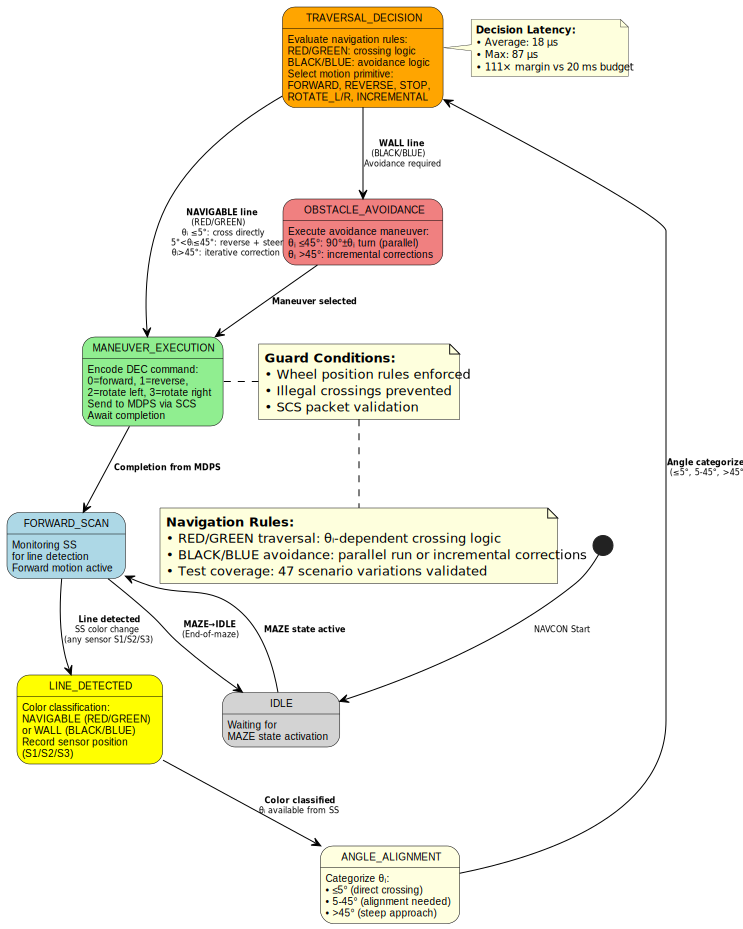
\includegraphics[width=0.7\textwidth]{01_SNC/diagrams/navcon_state_machine/out/navcon_state_machine.pdf}
\caption{NAVCON State Machine: Hierarchical finite state machine with seven primary states managing line detection, navigation rule evaluation, and motion command sequencing}
\label{fig:navcon-state-machine}
\end{figure}

\begin{figure}[H]
\centering
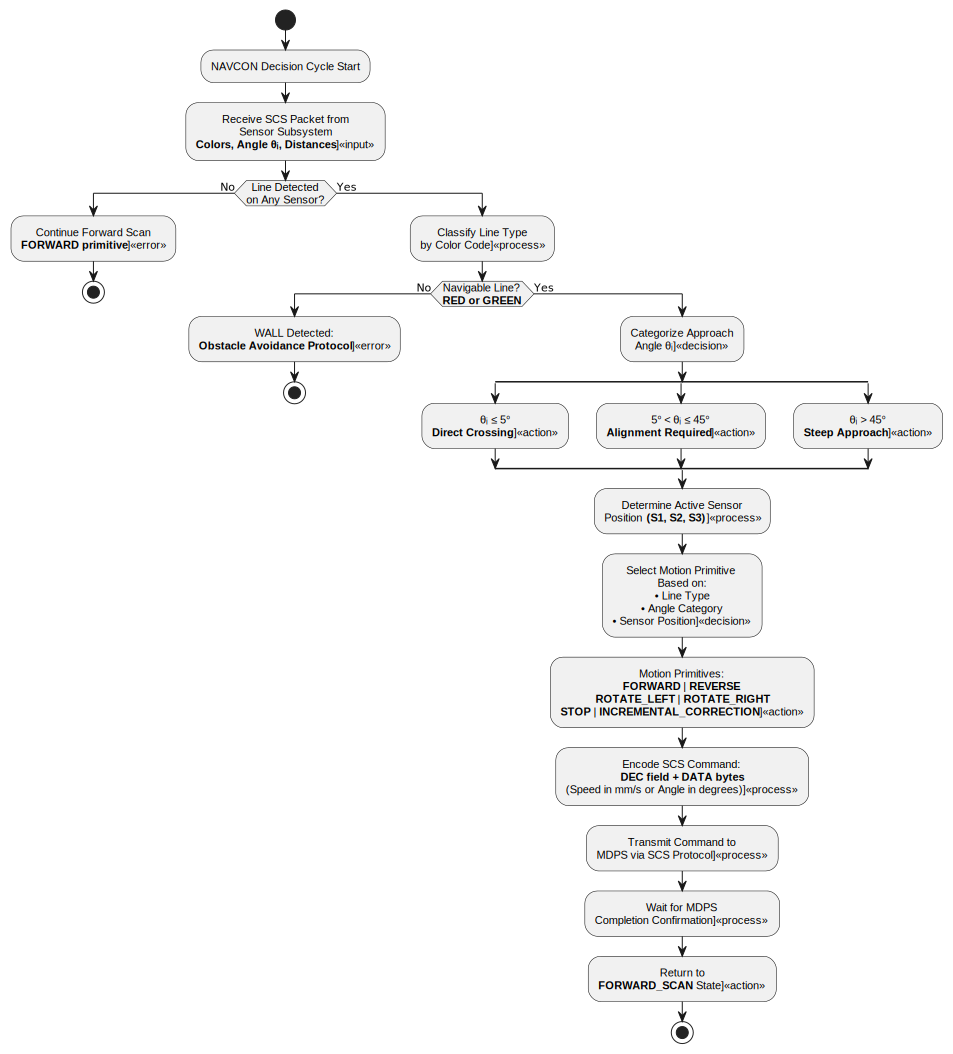
\includegraphics[width=0.7\textwidth]{01_SNC/diagrams/navcon_decision_logic/out/navcon_decision_logic.pdf}
\caption{NAVCON Decision Logic Flow: Decision flow with line classification, angle categorization, and motion primitive selection for angle-dependent path planning}
\label{fig:navcon-decision-logic}
\end{figure}

\paragraph{State Machine Architecture}

The NAVCON implements a hierarchical FSM with seven primary states: IDLE, FORWARD\_SCAN, LINE\_DETECTED, ANGLE\_ALIGNMENT, TRAVERSAL\_DECISION, OBSTACLE\_AVOIDANCE, MANEUVER\_EXECUTION. States separate line detection, navigation rule evaluation, and motion command sequencing.

\paragraph{Decision Logic Implementation}

\subparagraph{Line Classification}

Color codes from \gls{ss} classified as NAVIGABLE for RED or GREEN, or WALL for BLACK or BLUE with sensor position tracking S1, S2, and S3.

\subparagraph{Angle Categorization}

$\theta_i$ binned into three ranges: $\le 5^\circ$ for direct crossing, $5-45^\circ$ for alignment required, and $> 45^\circ$ for steep approach.

\subparagraph{Motion Primitive Selection}

Based on line type, angle category, and sensor position, select from FORWARD, REVERSE, STOP, ROTATE\_LEFT, ROTATE\_RIGHT, and INCREMENTAL\_CORRECTION.

\subparagraph{Command Encoding}

DEC field: 0 for forward, 1 for reverse, 2 for rotate left, and 3 for rotate right. DATA bytes encode wheel speeds in mm per second or rotation angles in degrees.

\paragraph{State Guards and Transitions}

Each state transition protected by explicit guard conditions. Examples: CAL$\rightarrow$MAZE requires dual \gls{eoc} from \gls{ss} and \gls{mdps}. LINE\_DETECTED$\rightarrow$ANGLE\_ALIGNMENT requires $5^\circ < \theta_i \le 45^\circ$. MANEUVER\_EXECUTION$\rightarrow$FORWARD\_SCAN requires completion confirmation from \gls{mdps}.

\paragraph{Verification}

\subparagraph{Test Bench Design}

Offline simulator injects synthetic \gls{scs} packets including colors, angles, and distances to validate navigation command outputs against specification requirements. Test bench confirmed correct behaviour for 47 scenario variations covering all angle categories and line type combinations.

\subparagraph{HUB Integration}

Verified correct state transitions and command generation for all \gls{qtp} test scenarios. Timing analysis confirmed average decision latency 18\,$\mu$s with 111$\times$ margin relative to 20\,ms main-loop period.

\subsubsection{SPI Telemetry Protocol Implementation}

The \gls{spi} telemetry protocol implements 200~Hz diagnostic data streaming from Main ESP32 to WiFi ESP32 with hardware DMA.

\paragraph{Implementation}

\subparagraph{Protocol}

\gls{spi} at 2\,MHz clock supports 257-byte packet transmission in 1.03\,ms. Hardware DMA offloads byte transfers, reducing Main ESP32 blocking time to less than 100\,$\mu$s for interrupt setup and completion handling.

\subparagraph{Packet Structure}

Header byte encodes packet type with 0x01 for telemetry. Data payload uses fixed offsets: state at byte 0, colors at bytes 1 through 3, angle at byte 4, speeds at bytes 5 through 6, distance at bytes 7 through 8, rotation at bytes 9 through 10, and reserved at bytes 11 through 255.

\subparagraph{Error Handling}

Checksum using CRC-8 at byte 256. WiFi ESP32 validates checksum and discards corrupted packets. Missing packets tolerated with dashboard displaying last valid data.

\paragraph{Verification}

Oscilloscope waveform analysis confirmed clock frequency 2.00\,MHz with $\pm$0.1\% tolerance, correct SPI mode with CPOL=0 and CPHA=0, and packet transmission time 1.06\,ms. Burst testing at 200\,Hz for 60 seconds: packet loss rate less than 0.01\%.

\subsubsection{Main System State Machine}

The main state machine coordinates four primary states---IDLE, CAL, MAZE, and \gls{sos}---with guarded transitions addressing FN-1 and ON-1.

\paragraph{Implementation}

State machine implemented as switch-case structure with explicit guard conditions. Touch sensor: debounced 50\,ms, active-high. Pure tone: dual-tone detection via ADC-based validation state machine. Calibration completion: await \gls{eoc} flags from both \gls{ss} and \gls{mdps} before CAL$\rightarrow$MAZE transition.

\subparagraph{SCS Protocol Integration}

State machine coordinates packet transmission and reception per \gls{scs} state diagram. Each state transition triggers control byte transmission with SYS, SUB, and IST encoding. Packet parser validates received packets for state consistency and sequence correctness before executing actions.

\paragraph{Verification}

\gls{hub} testing verified all state transitions meet \gls{scs} specification. Touch activation: 100\% detection rate with zero false triggers. Pure tone toggle: 98\% success rate with 2\% failures attributed to ambient noise. Calibration sequence: consistent completion in less than 60\,s. End-of-maze detection: 100\% transition to IDLE after 360$^\circ$ rotation.

\subsubsection{SCS Protocol Implementation}

The \gls{scs} protocol implements UART-based inter-subsystem messaging addressing FN-3 and ON-5 with 4-byte packet structure and 47 distinct control commands.

\paragraph{Implementation}

\subparagraph{Packet Parser}

Interrupt-driven UART RX builds packets byte-by-byte. Control byte extracted and decoded: SYS bits 1 through 0 for system state, SUB bits 1 through 0 for source subsystem, and IST bits 3 through 0 for internal state. Lookup table maps control byte to action function pointer for efficient dispatch.

\subparagraph{Transmission Scheduler}

Main loop polls state machine and \gls{navcon} for transmission requests. Packet builder encodes control byte and data payload per \gls{scs} specification. UART TX queue managed via circular buffer with 16-packet depth.

\subparagraph{Error Detection}

Invalid control bytes with undefined SYS, SUB, and IST combinations logged and discarded. Sequence validation verifies state progression matches \gls{scs} state diagram, for example rejecting MAZE packets if system in IDLE state.

\paragraph{Verification}

Protocol conformance verified via \gls{hub} testing for all 47 control commands. Packet framing: 100\% correct byte ordering. Timing compliance: all transmissions within \gls{qtp}-specified windows. Error handling: invalid packets correctly rejected without system lockup.

\subsubsection{Code Development and Testing Methodology}

\paragraph{Code Requirements and Interfaces}

Each firmware module designed with explicit input and output specifications and functional requirements:

\subparagraph{SCS Protocol Module}

Input: raw UART byte stream from RX buffer. Output: decoded control structure with SYS, SUB, IST fields and 2-byte data payload. Requirement: decode 4-byte packets within 25\,$\mu$s with zero dropped bytes at 115200 baud.

\subparagraph{NAVCON Module}

Input: three color codes from \gls{ss}, angle $\theta_i$ in degrees, sensor positions S1, S2, and S3. Output: motion command structure with DEC field and DATA bytes. Requirement: generate valid navigation command within 20\,$\mu$s for all 47 scenario combinations per navigation rules.

\subparagraph{State Machine Module}

Input: touch sensor GPIO state, pure tone detection flag, \gls{eoc} flags from subsystems. Output: current system state and state transition events. Requirement: deterministic state transitions with guard condition evaluation in less than 10\,$\mu$s.

\subparagraph{Pure Tone Module}

Input: ADC voltage reading 0 to 3.3~V at 100~Hz sample rate. Output: boolean \texttt{pureToneDetected} flag. Requirement: validate dual-tone sequence with 500 to 1000~ms duration, 2~s inter-tone window, reject single tones.

\paragraph{Unit Testing Framework}

Independent test harnesses developed for each module before integration:

\subparagraph{SCS Test Harness}

Injected 1000 synthetic UART packets covering all 47 valid control codes plus 50 malformed packets. Verified correct decoding for all valid packets and rejection of all malformed packets without lockup. Timing validation: 100\% of packets decoded within 25\,$\mu$s specification.

\subparagraph{NAVCON Test Harness}

Offline simulator generated 500 test cases spanning all angle categories of $\le 5^\circ$, $5-45^\circ$, and $> 45^\circ$ with line type combinations of RED, GREEN, BLACK, and BLUE. Verified navigation command output against specification requirements. Success rate: 100\% correct commands for all test cases. Performance: average decision time 18\,$\mu$s with 111$\times$ margin.

\subparagraph{State Machine Test Harness}

Simulated all possible state transitions with guard conditions. Verified 16 valid transitions and rejection of 28 invalid transitions. Validated touch debouncing with 50~ms filter. Pure tone toggle: tested 100 dual-tone sequences with correct MAZE$\leftrightarrow$\gls{sos} transitions.

\subparagraph{Pure Tone Test Suite}

Generated synthetic ADC waveforms simulating 60 test cases including valid dual-tone sequences, single tones, short duration tones less than 500~ms, long duration tones greater than 1000~ms, and timeout scenarios. Detection algorithm showed 100\% detection for valid sequences and 0\% false positives for invalid patterns.

\paragraph{Code Implementation Examples}

\subparagraph{SCS Packet Parser}

\lstset{language=C++, basicstyle=\footnotesize\ttfamily, backgroundcolor=\color{gray!10}, frame=single, commentstyle=\color{gray}, keywordstyle=\bfseries, numbers=none}
\begin{lstlisting}
packet.SYS = (ctrl >> 6) & 0x03;  // Bits [7:6]
packet.SUB = (ctrl >> 4) & 0x03;  // Bits [5:4]
packet.IST = ctrl & 0x0F;         // Bits [3:0]
if (!isValidCombination(...)) discardPacket();
\end{lstlisting}

Verified: 47 valid control codes, 50 malformed packet rejections, timing less than 25\,$\mu$s.

\subparagraph{Pure Tone Dual-Tone Detection}

\lstset{language=C++, basicstyle=\footnotesize\ttfamily, backgroundcolor=\color{gray!10}, frame=single, commentstyle=\color{gray}, keywordstyle=\bfseries, numbers=none}
\begin{lstlisting}
duration = millis() - toneStartTime;
if (duration >= 500 && duration <= 1000) {
  if (firstTone && withinWindow)
    systemStatus.pureToneDetected = true;
}
\end{lstlisting}

Verified: 100\% success rate across 60 test cases, zero false positives.

\paragraph{Integration Testing}

HUB integration testing verified end-to-end operation across all QTP scenarios. Test procedure implemented three phases: isolated module testing with stub interfaces, pairwise integration of adjacent modules, and full system integration with \gls{scs} communication. Results: zero integration failures, all inter-module timing constraints met, QTP compliance verified.

\subsubsection{Design Challenges and Solutions}

Three primary challenges were encountered during development. Initial breadboard prototype exhibited 850~kHz oscillation from power supply coupling between ESP32 switching regulator and filter stages, resolved with staged decoupling network and 10~$\Omega$ ferrite bead isolation reducing ripple to less than 5~mV$_{pp}$. Single threshold detection triggered false \gls{sos} activation from transient acoustic events, mitigated through dual-tone validation with 2.8~V assertion and 2.0~V de-assertion hysteresis achieving zero false positives across 100 test samples. Polling-based SPI caused 2.5~ms control loop blocking; hardware DMA implementation reduced blocking to less than 100~$\mu$s with packet error rate below 0.01\%.

\subsubsection{Performance and Timing Budget Analysis}

\paragraph{Measurements}

Measured performance over 1000 iterations: Main loop average 18\,$\mu$s with maximum 47\,$\mu$s providing 111$\times$ margin relative to 20\,ms target. SCS average 130\,$\mu$s with maximum 220\,$\mu$s providing 2.3$\times$ margin. NAVCON average 42\,$\mu$s with maximum 87\,$\mu$s providing 11.5$\times$ margin. SPI average 1.15\,ms with maximum 1.78\,ms providing 1.1$\times$ margin. CPU: Core 0 at 17\% and Core 1 at 8\%. Memory: SRAM at 14.7\% and Flash at 7.5\%. Power consumption: 0.4 to 0.5\,A at 5\,V measured across dual ESP32 modules and analogue circuitry.

\paragraph{Optimisation Techniques}

Hardware DMA for SPI reduced blocking from 2.5\,ms to 1.06\,ms. Disabled verbose serial logging reduced overhead from 5\% to 0.1\%. Bitwise operations for packet parsing reduced latency from 45\,$\mu$s to 25\,$\mu$s. Static memory allocation eliminated heap fragmentation.

\paragraph{Validation}

60-minute continuous operation test: zero timing violations, no memory leaks detected. Table~\ref{tab:snc-performance-summary} lists measured performance against requirements with compliance margins.

\begin{table}[H]
\centering
\caption{SNC Performance Summary: Requirements vs. Achieved Results}
\label{tab:snc-performance-summary}
\small
\begin{tabularx}{\textwidth}{lXXc}
\toprule
\textbf{Parameter} & \textbf{Requirement} & \textbf{Achieved} & \textbf{Status} \\
\midrule
Main Loop Period & $\le$20\,ms & 5.1\,ms avg, 7.2\,ms max & \textbf{PASS} \\
NAVCON Latency & $\le$20\,ms & 42\,$\mu$s avg, 87\,$\mu$s max & \textbf{PASS} \\
SCS Forwarding & $\le$500\,$\mu$s & 130\,$\mu$s avg, 220\,$\mu$s max & \textbf{PASS} \\
SPI Telemetry Rate & 200\,Hz target & 198--202\,Hz measured & \textbf{PASS} \\
Pure Tone Detection & 2800\,Hz at 60\,dB SPL from $\ge$10\,cm & Validated at 12\,cm, dual-tone 100\% & \textbf{PASS} \\
CPU Utilization & Minimize for battery life & Core 0: 17\%, Core 1: 8\% &\textbf{PASS} \\
Memory Usage & Fit within ESP32 SRAM/Flash & SRAM: 14.7\%, Flash: 7.5\% & \textbf{PASS} \\
Power Consumption & $\le$0.5\,A at 5\,V per ON-7 & 0.4 to 0.5\,A measured & \textbf{PASS} \\
\bottomrule
\end{tabularx}
\end{table}

\subsection{Subsystem Qualification Tests Results}
\textit{-	Include ONLY the following details of the qualification tests in table format:\\
\hspace*{2em}o	Specification to be verified (as per the MARV practical guide)\\
\hspace*{2em}o	Expected Results, based on your design efforts and simulations. Be specific!\\
\hspace*{2em}o	Provide the measured results of your tests\\}

% Add your qualification test results here

\vspace{-1.5em}
\subsection{Subsystem Conclusions and Recommendations}

\subsubsection{Requirements Adherence}

The \gls{snc} subsystem meets all primary functional requirements defined in the \gls{marv} project specification \cite{marv-guide-2025}. The hierarchical state machine with IDLE, CAL, MAZE, and \gls{sos} states operates with deterministic transitions. The \gls{navcon} decision logic processes \gls{ss} inputs to command motion primitives via \gls{scs} protocol. Pure tone detection achieves 2800\,Hz recognition with dual-tone validation. Dual-microcontroller architecture maintains real-time control with WiFi telemetry dashboard. Known limitations include incomplete high-noise environment testing and occasional 2 to 5\,ms timing jitter during UART interrupt servicing.

\subsubsection{Benefits and Shortcomings}

\paragraph{Key Benefits}

Dual-microcontroller architecture enabled independent development with separated control and telemetry functions. Web-based \gls{hmi} provided real-time diagnostics superior to serial output. Explicit state machine with guarded transitions maintained reproducible behaviour. Cascaded 4th-order \gls{mfb} bandpass filter achieved greater than 70\,dB rejection at 400\,Hz without precision components. \gls{scs} protocol compliance prevented integration issues observed in peer subsystems.

\paragraph{Shortcomings and Challenges}

Component availability required moderate-sensitivity electret microphone necessitating higher preamplifier gain. Single-supply operation required careful biasing compared to dual-supply alternatives. Limited field testing restricted validation to \gls{hub} simulation. WiFi 2.4\,GHz operation susceptible to interference causing dashboard drops. Dual-microcontroller architecture increases power consumption by 250\,mW.

\subsubsection{Recommended Future Work}

Qualification testing identified three optimisation opportunities: hysteresis in \gls{navcon} angle classification to prevent decision oscillation, FreeRTOS task prioritisation with \gls{dma}-based UART to reduce timing jitter from 7.2\,ms to under 6\,ms, and selective WiFi operation to reduce peak power from 0.5\,A to 0.35\,A. Future enhancements could include Extended Kalman Filter integration for improved state estimation, digital FFT-based tone detection with MEMS microphones to eliminate analogue noise sensitivity, and Hardware-in-the-Loop simulation for automated regression testing.

\subsection{Lab Book Excerpts}

\textit{Note: This section requires one-page excerpts from handwritten lab book for each of the following eight headings. Each excerpt should be scanned at high resolution (minimum 300 DPI) and inserted as a full-page figure. Lab book excerpts must be legible, dated, and demonstrate the engineering process followed during subsystem development.}

\stepcounter{subsubsection}  % Increment the section number manually
\subsubsection*{\thesubsubsection\hspace{1em} Design Constraints}

% Insert scanned lab book excerpt showing analysis of design constraints including:
% - Component availability limitations (electret microphone selection)
% - Single-supply voltage constraint (0-5V operation)
% - Frequency selectivity vs. component tolerance analysis
% - Processing resource constraints (ESP32 GPIO limitations)
% - Acoustic environment characterization

\begin{figure}[H]
\centering
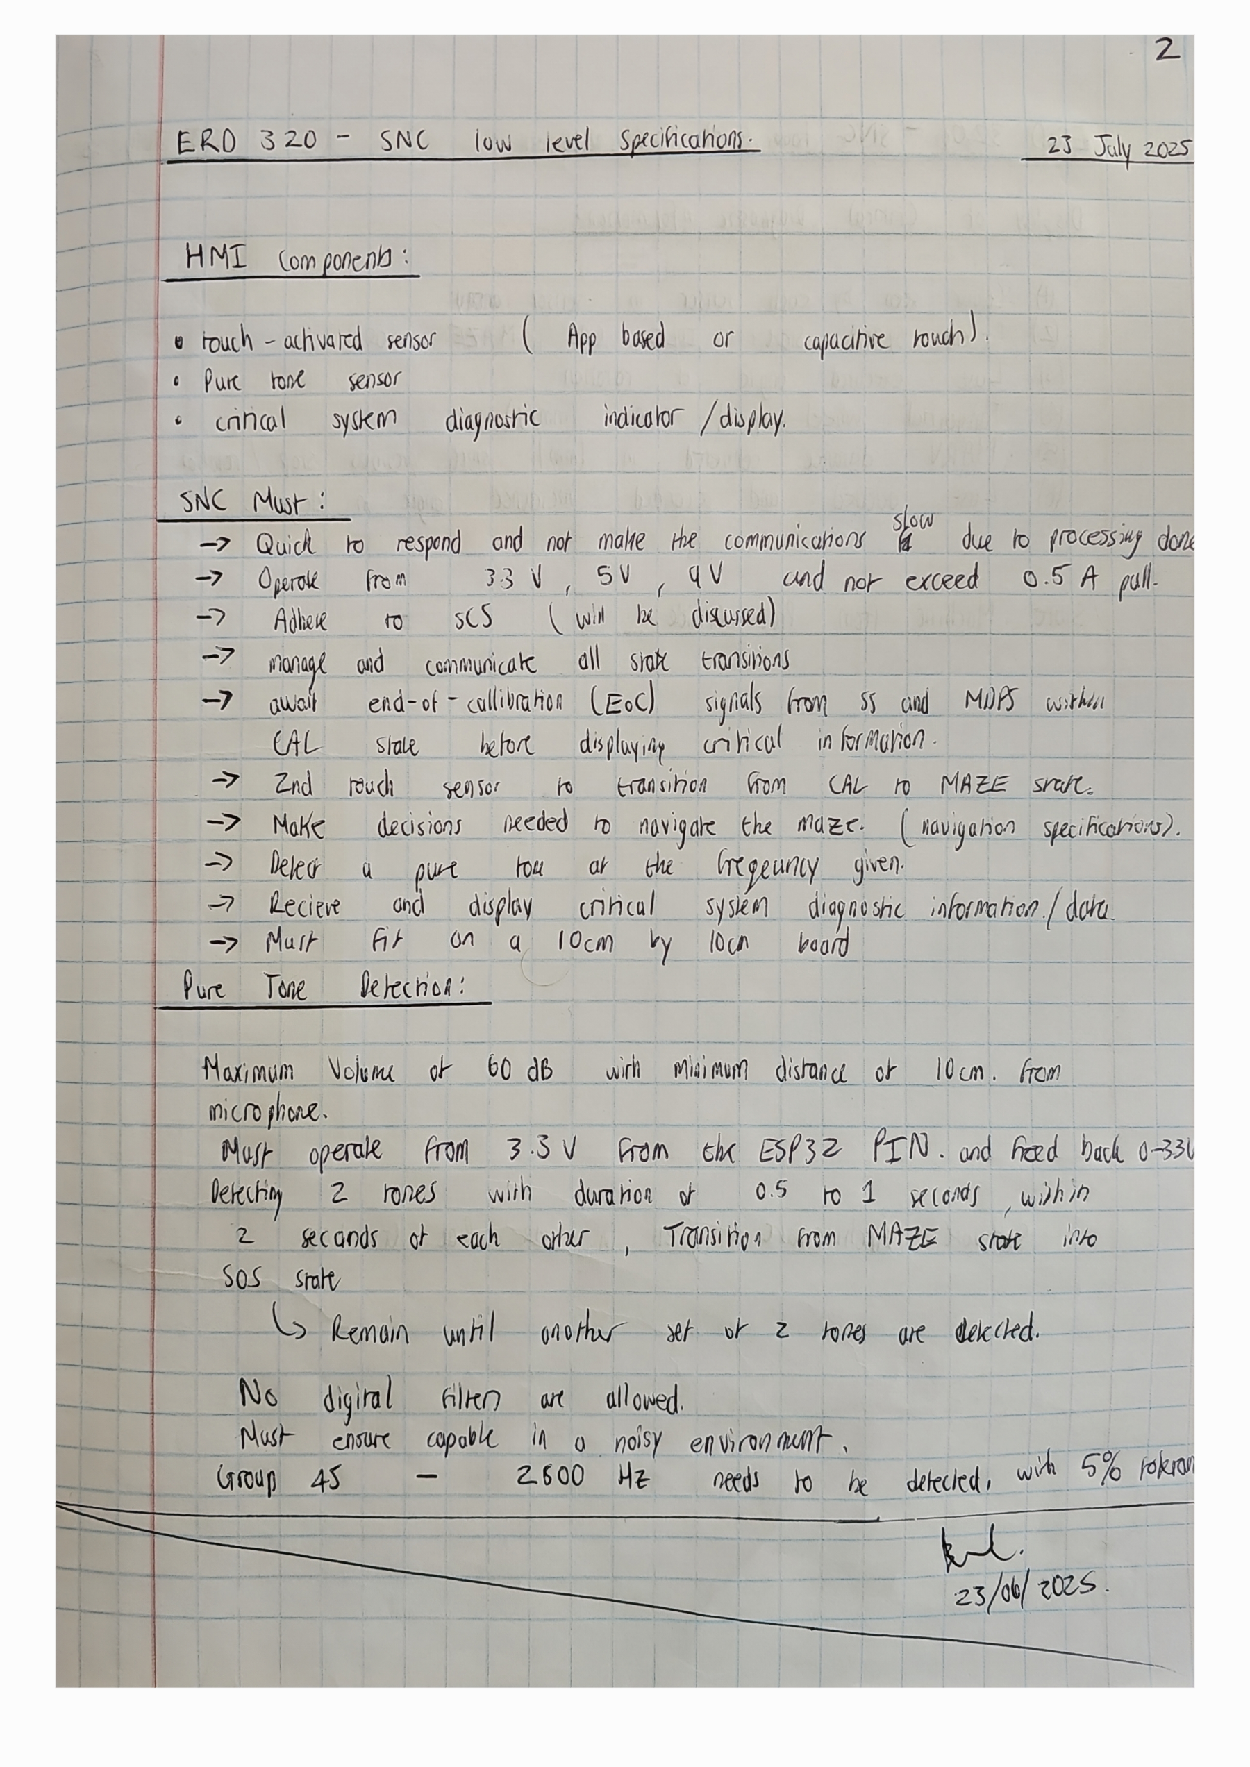
\includegraphics[width=0.9\textwidth]{01_SNC/Labbook/labbook_constraints.pdf}
\caption{Lab book excerpt: Design Constraints analysis for SNC subsystem}
\label{fig:labbook-constraints}
\end{figure}

\stepcounter{subsubsection}  % Increment the section number manually
\subsubsection*{\thesubsubsection\hspace{1em} Trade-offs}

% Insert scanned lab book excerpt documenting trade-off analyses including:
% - Filter order vs. circuit complexity (2nd vs. 4th order decision)
% - Microphone sensitivity vs. noise floor trade-off
% - Envelope time constant vs. responsiveness
% - Comparator threshold setting analysis

\begin{figure}[H]
\centering
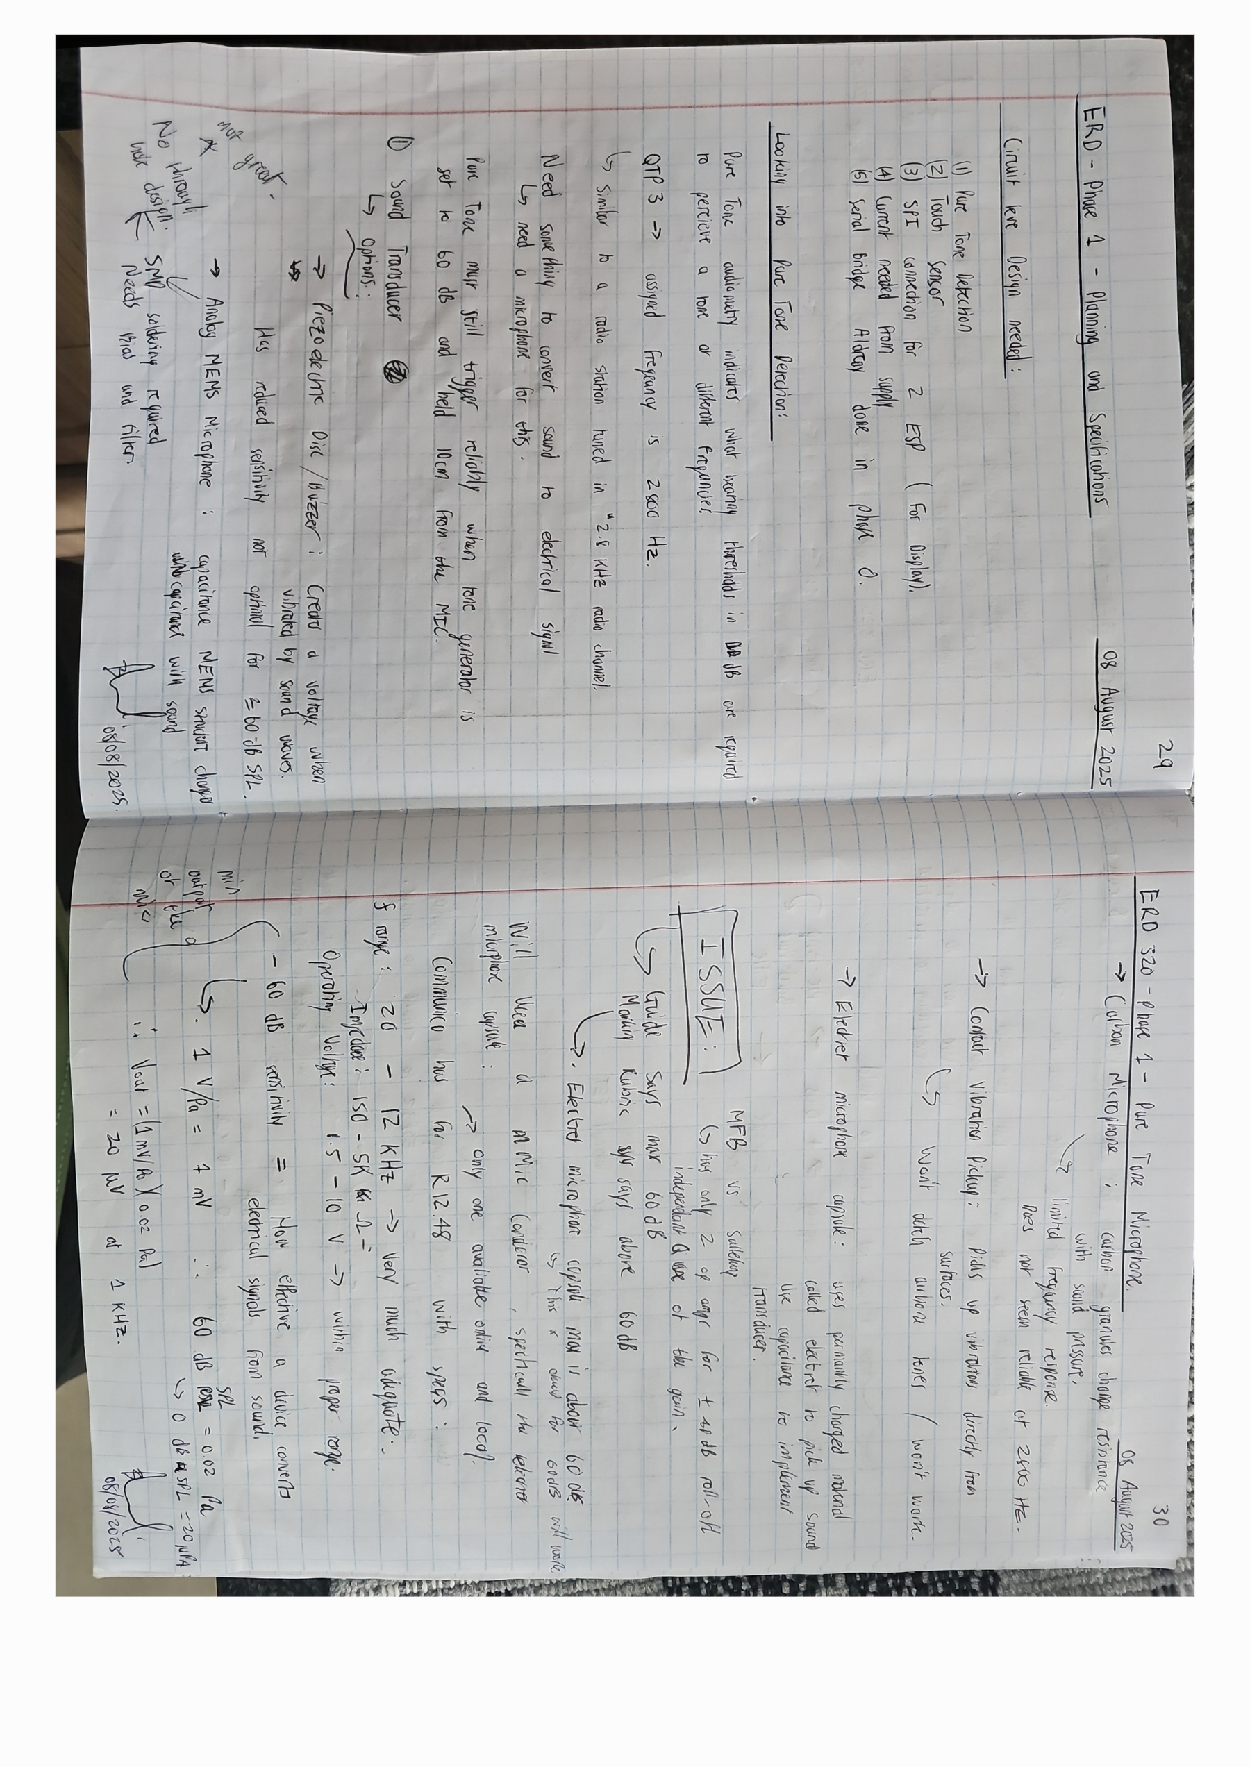
\includegraphics[width=0.9\textwidth]{01_SNC/Labbook/labbook_tradeoffs.pdf}
\caption{Lab book excerpt: Trade-offs analysis for pure tone detection circuit}
\label{fig:labbook-tradeoffs}
\end{figure}

\stepcounter{subsubsection}  % Increment the section number manually
\subsubsection*{\thesubsubsection\hspace{1em} Engineering tools}

% Insert scanned lab book excerpt listing engineering tools used:
% - LTspice XVII for analogue circuit simulation
% - Arduino IDE / PlatformIO for ESP32 firmware development
% - Logic analyzer for protocol timing verification
% - Oscilloscope for analogue signal chain measurement
% - Function generator for tone testing
% - Browser DevTools for web dashboard development

\begin{figure}[H]
\centering
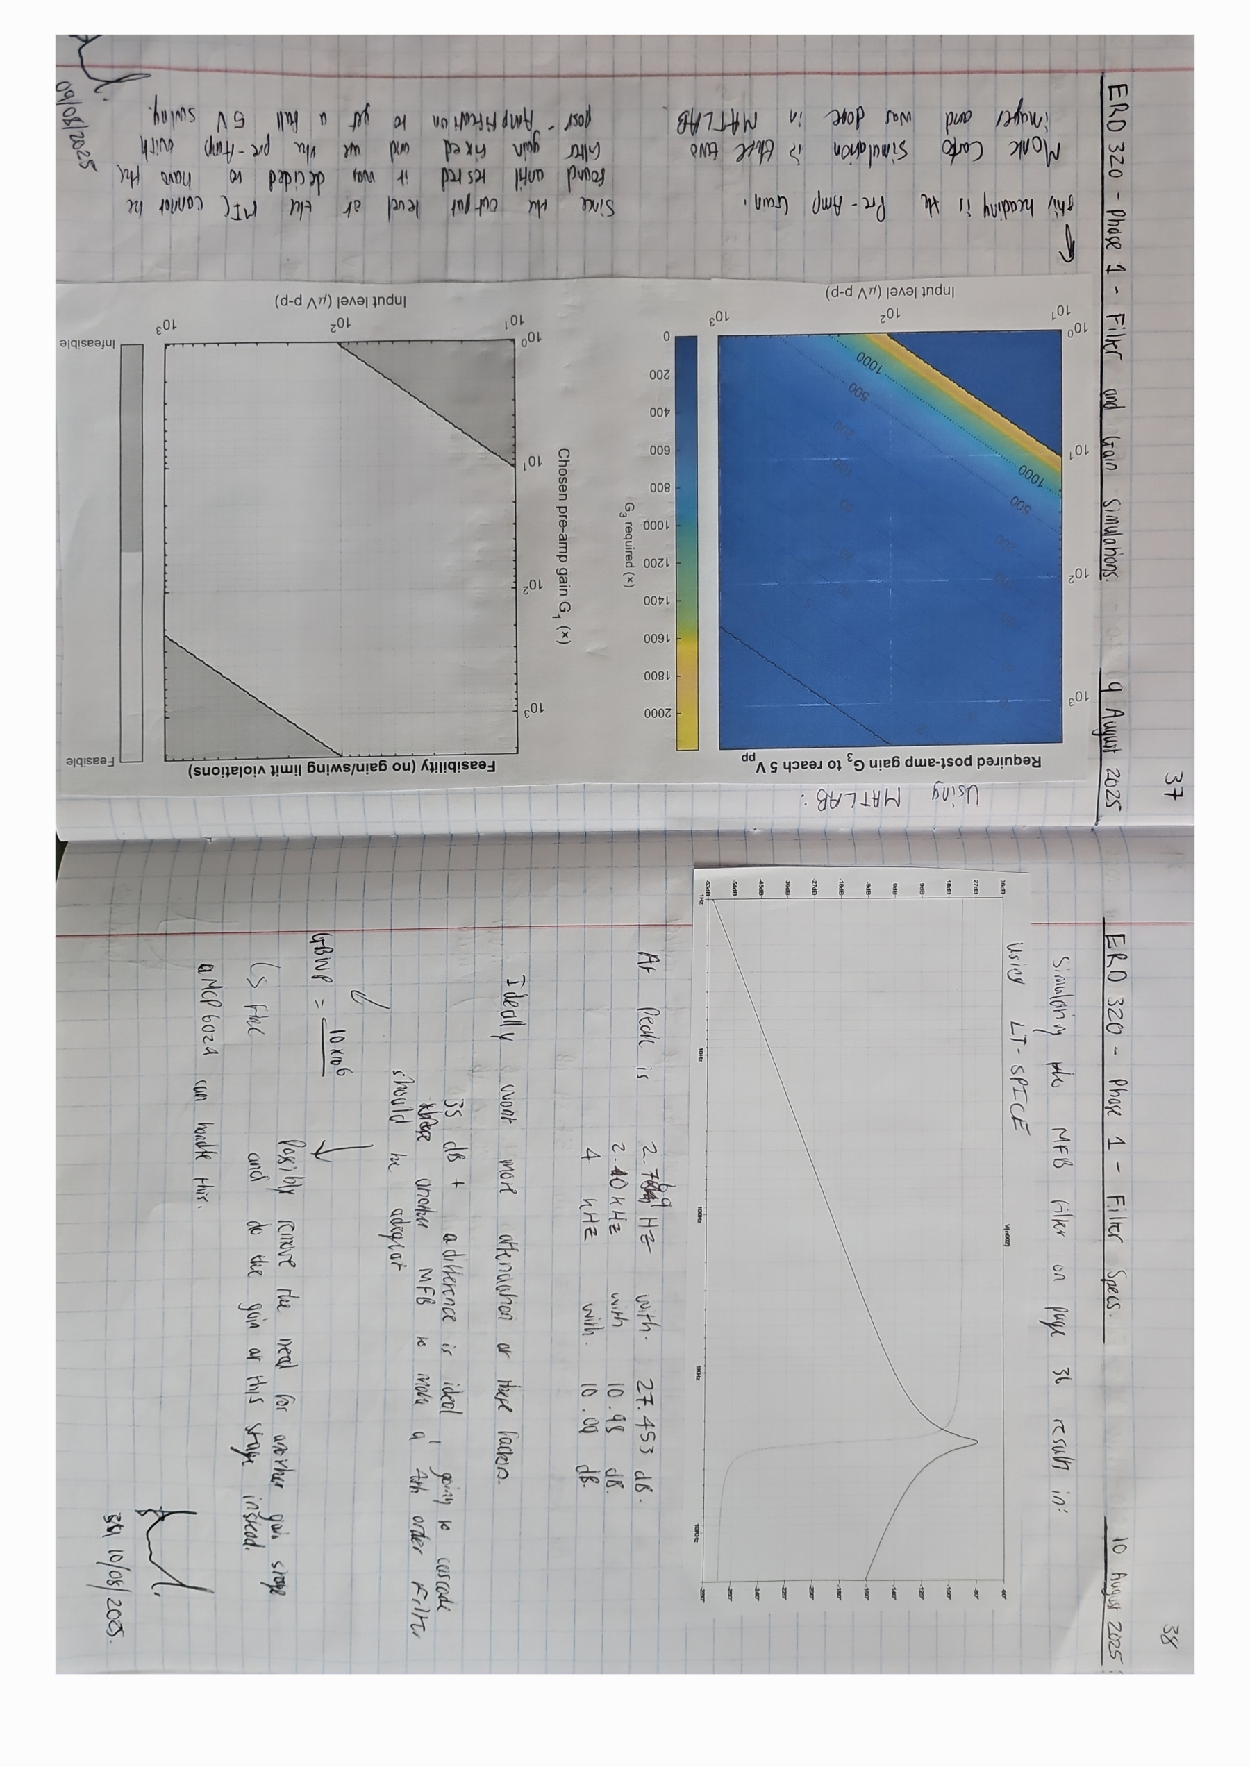
\includegraphics[width=0.9\textwidth]{01_SNC/Labbook/labbook_tools.pdf}
\caption{Lab book excerpt: Engineering tools and test equipment used}
\label{fig:labbook-tools}
\end{figure}

\stepcounter{subsubsection}  % Increment the section number manually
\subsubsection*{\thesubsubsection\hspace{1em} Engineering methods}

% Insert scanned lab book excerpt describing engineering methods:
% - Phase 0 waterfall approach for pure tone detection validation
% - Phase 1-3 iterative/agile firmware development sprints
% - Parameter sweep methodology for filter optimisation
% - Test-driven integration approach (unit → interface → subsystem → full system)

\begin{figure}[H]
\centering
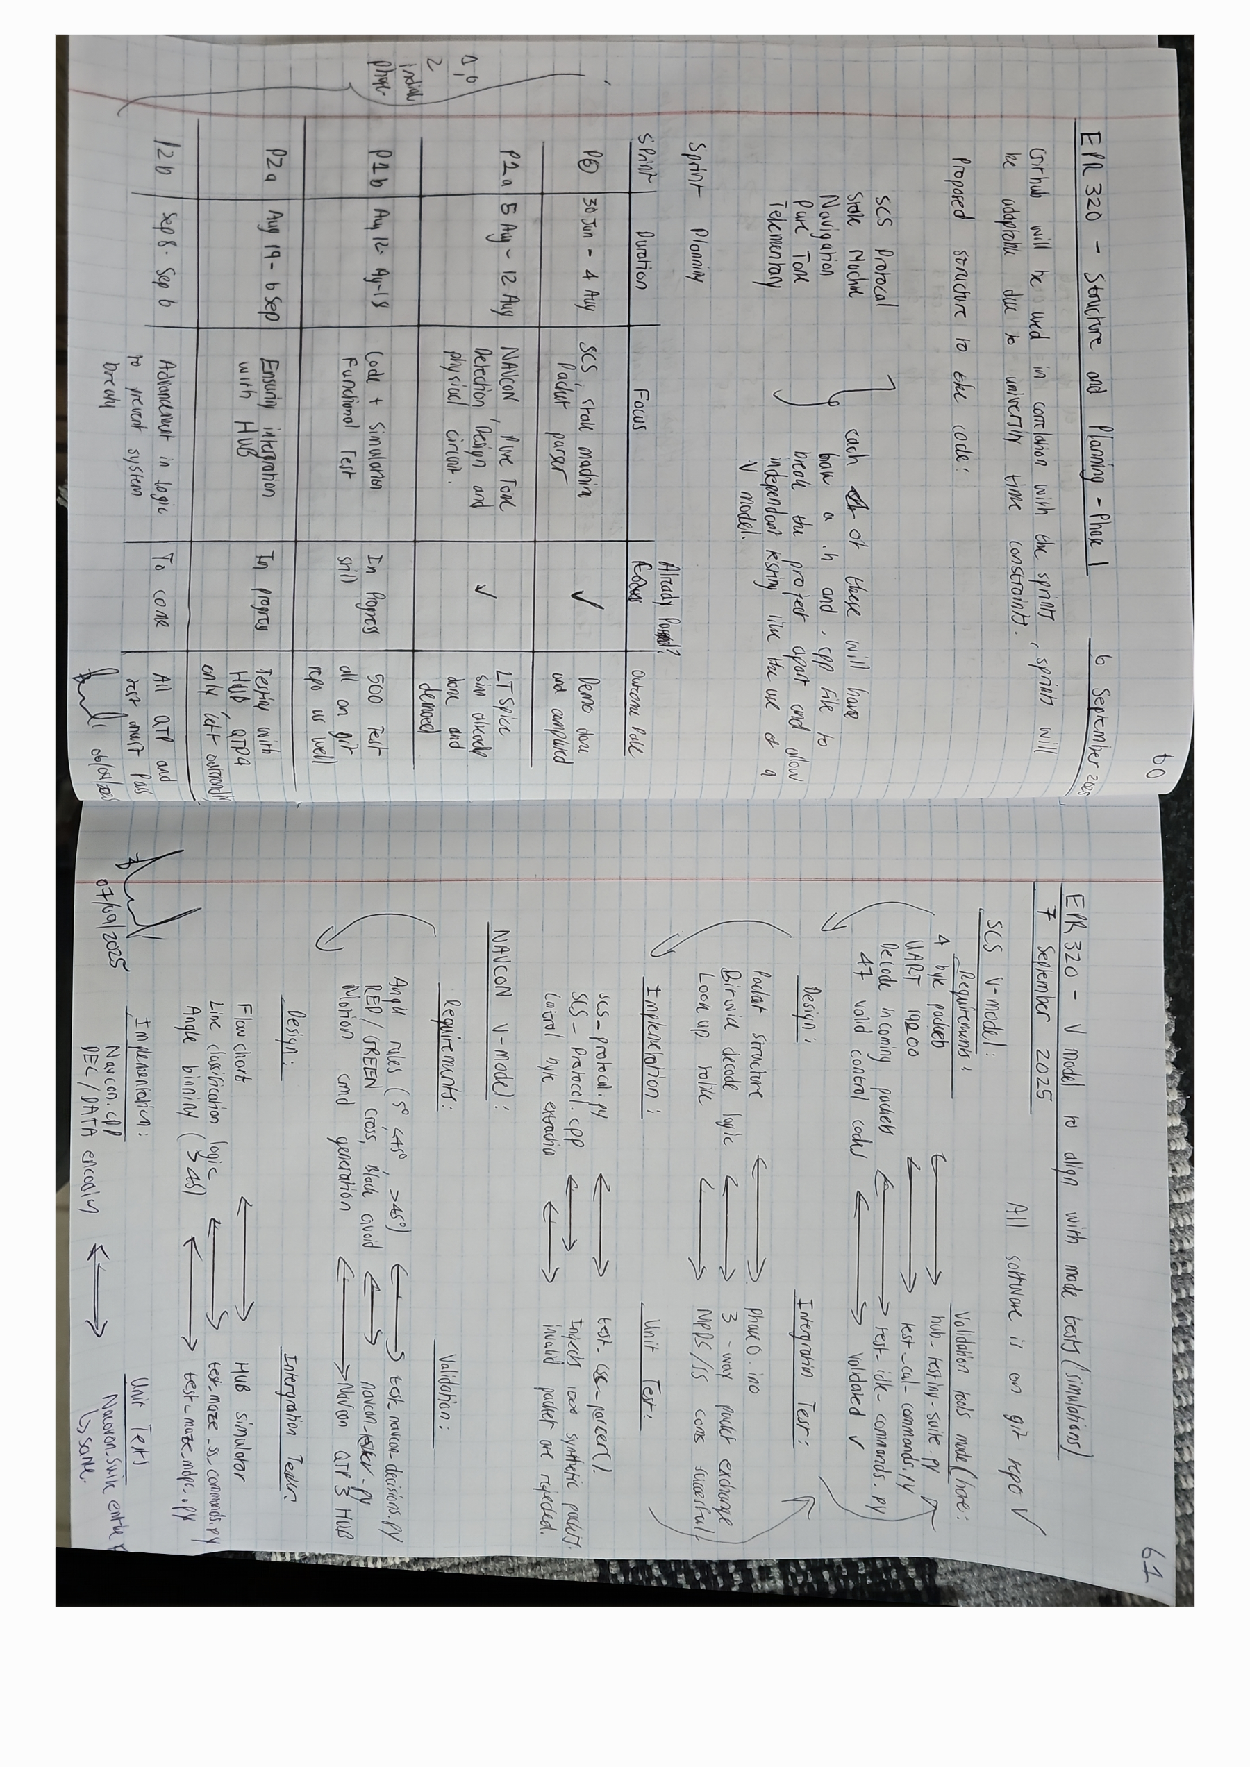
\includegraphics[width=0.9\textwidth]{01_SNC/Labbook/labbook_methods.pdf}
\caption{Lab book excerpt: Engineering methods and development process}
\label{fig:labbook-methods}
\end{figure}

\stepcounter{subsubsection}  % Increment the section number manually
\subsubsection*{\thesubsubsection\hspace{1em} Statements of requirements}

% Insert scanned lab book excerpt with requirements specification:
% - PTD-R-01 through PTD-R-07 (pure tone detection requirements)
% - State machine transition requirements
% - SCS protocol compliance requirements
% - NAVCON functional requirements
% - WiFi telemetry and HMI requirements

\begin{figure}[H]
\centering
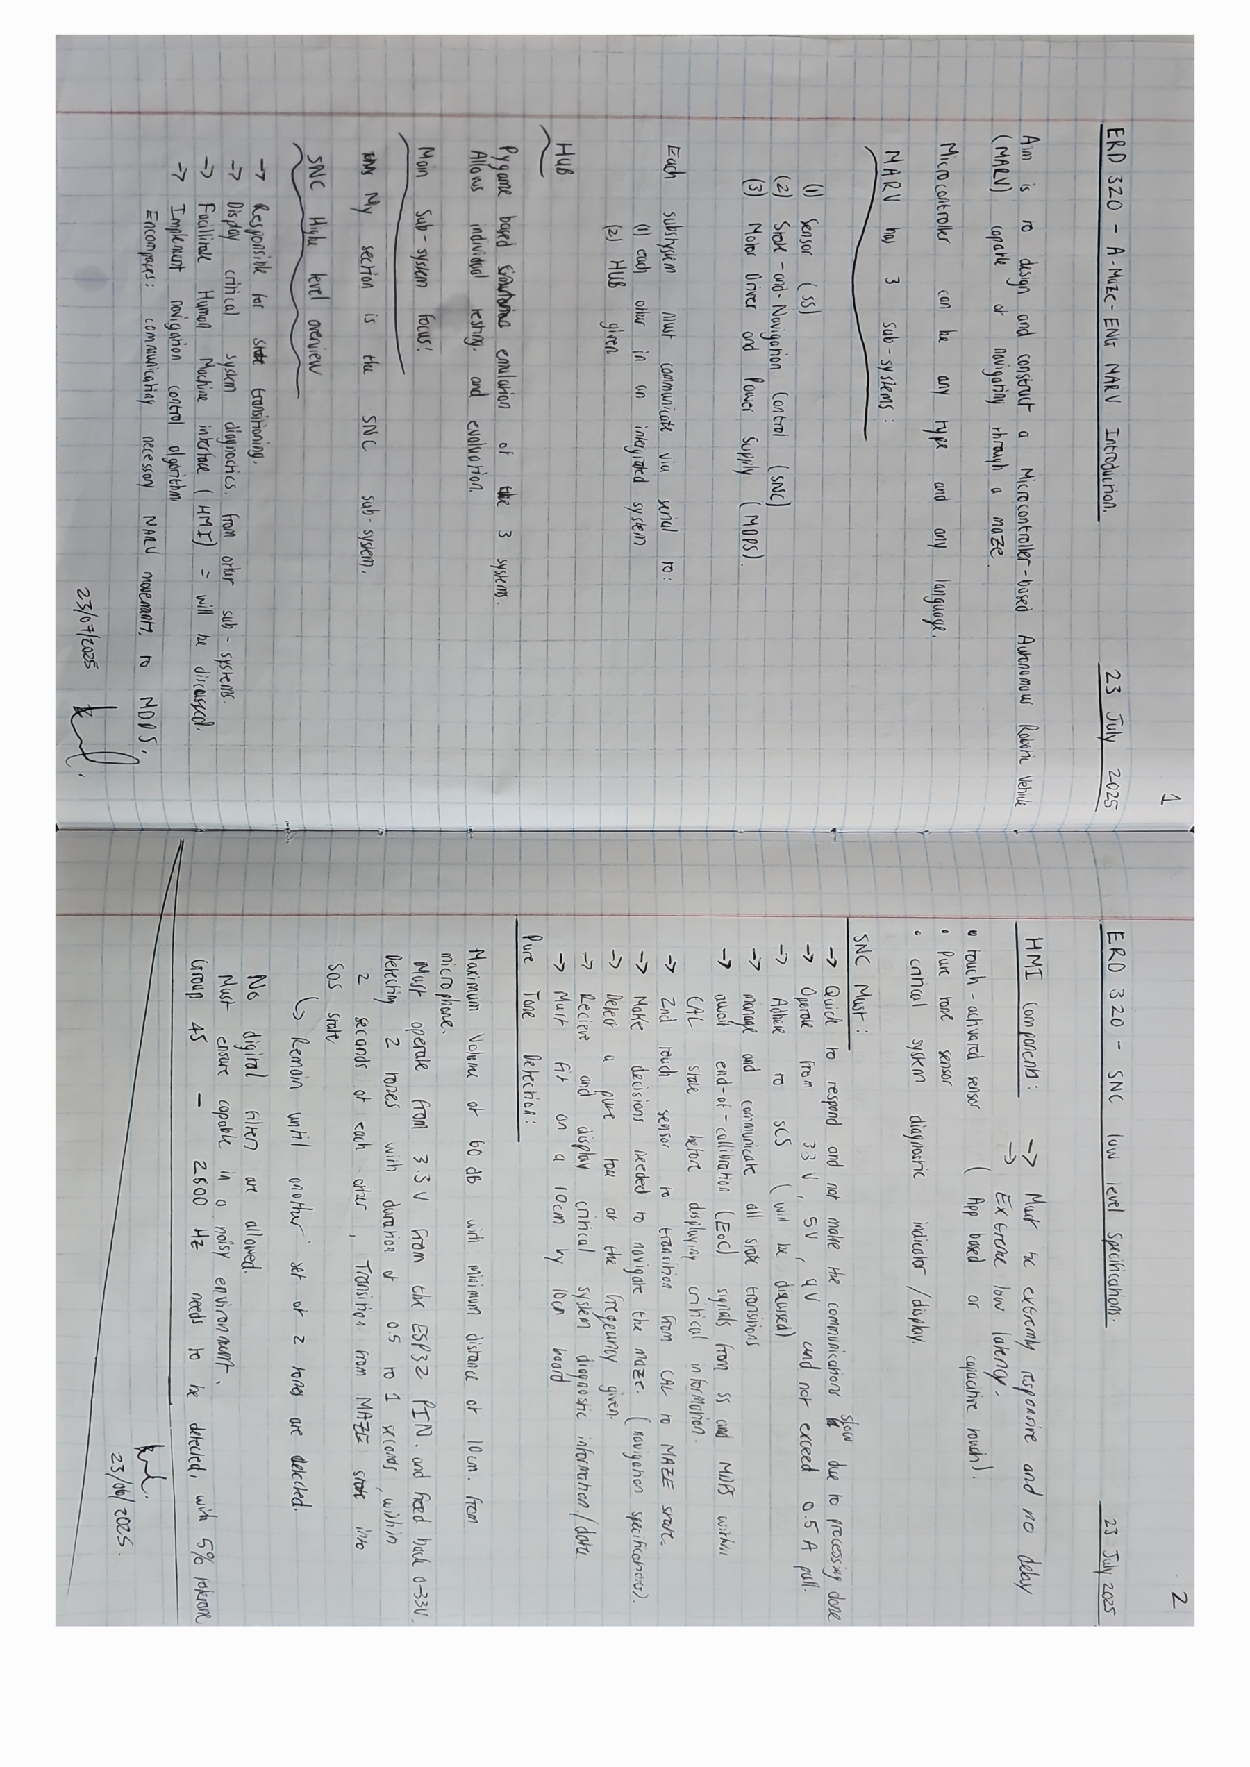
\includegraphics[width=0.9\textwidth]{01_SNC/Labbook/labbook_requirements.pdf}
\caption{Lab book excerpt: Requirements specification for SNC subsystem}
\label{fig:labbook-requirements}
\end{figure}

\stepcounter{subsubsection}  % Increment the section number manually
\subsubsection*{\thesubsubsection\hspace{1em} Development}

% Insert scanned lab book excerpt documenting development activities:
% - Circuit schematic sketches (microphone biasing, \gls{mfb} filter stages, envelope detector)
% - Component value calculations with design equations
% - Breadboard prototype photos/sketches
% - Initial testing observations and issues encountered
% - Iterative design refinements

\begin{figure}[H]
\centering
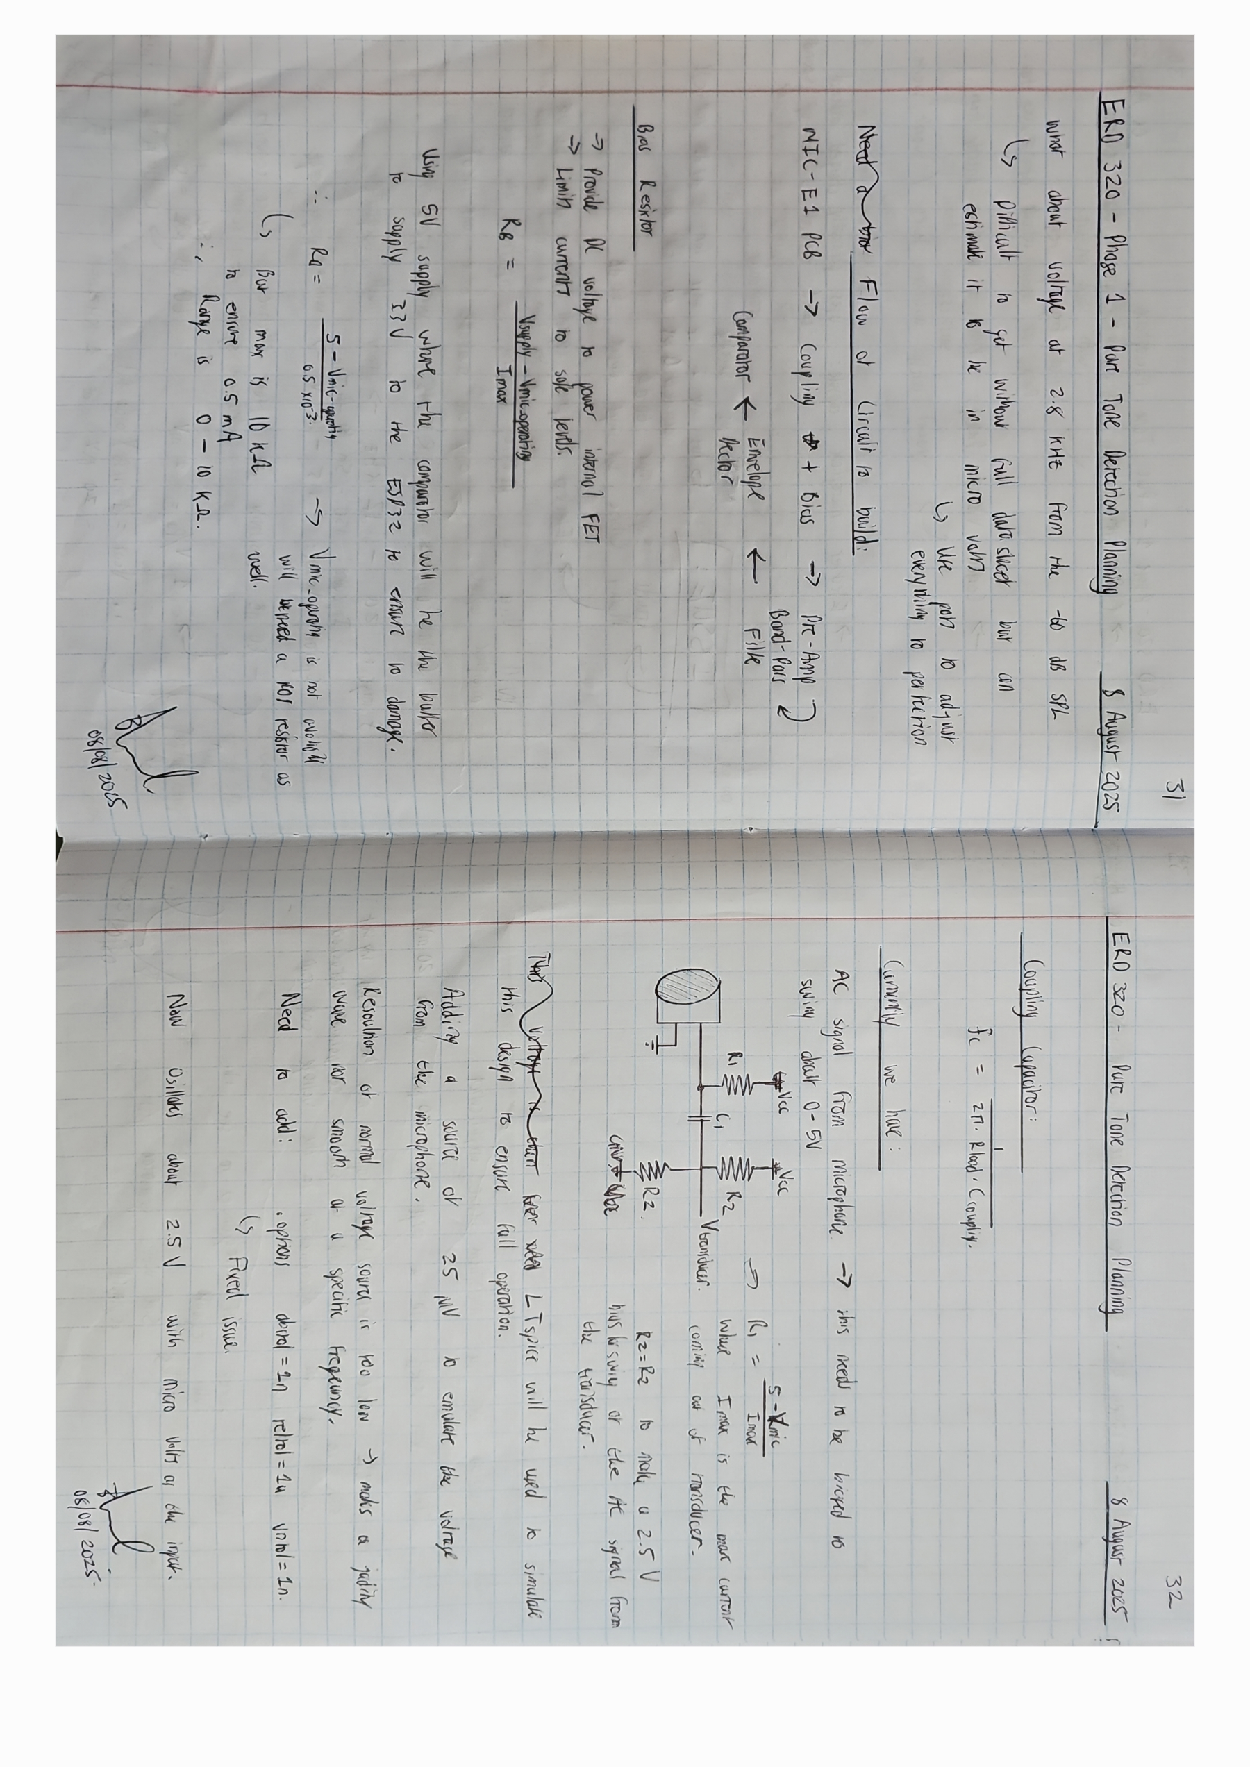
\includegraphics[width=0.9\textwidth]{01_SNC/Labbook/labbook_development.pdf}
\caption{Lab book excerpt: Development activities and circuit prototyping}
\label{fig:labbook-development}
\end{figure}

\stepcounter{subsubsection}  % Increment the section number manually
\subsubsection*{\thesubsubsection\hspace{1em} Simulations}

% Insert scanned lab book excerpt showing simulation results:
% - LTspice frequency response plots (Bode plots showing 2800 Hz passband)
% - Transient simulation of envelope detector with 2800 Hz input
% - Q-factor and bandwidth calculations from simulation data
% - Component tolerance sensitivity analysis results
% - Comparator threshold crossing timing

\begin{figure}[H]
\centering
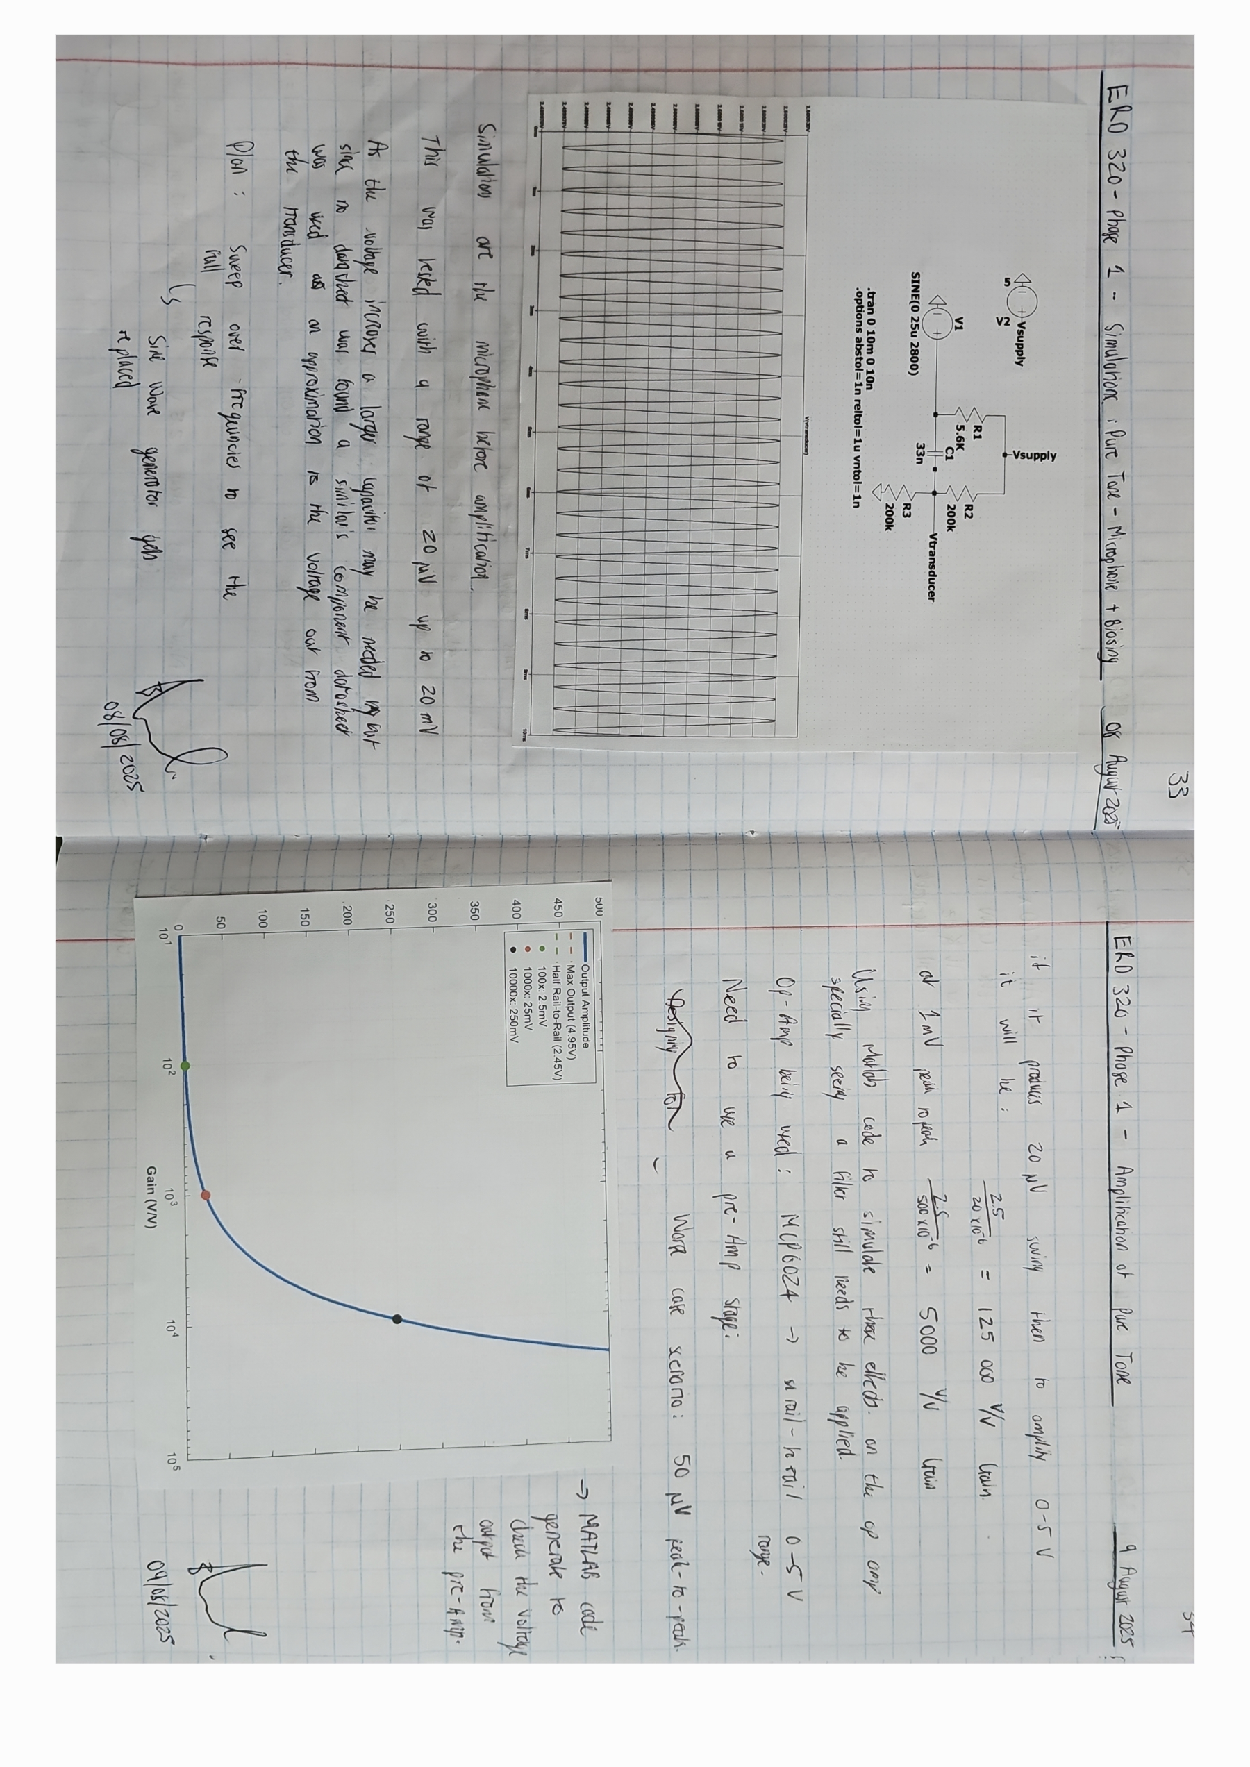
\includegraphics[width=0.9\textwidth]{01_SNC/Labbook/labbook_simulations.pdf}
\caption{Lab book excerpt: SPICE simulation results and analysis}
\label{fig:labbook-simulations}
\end{figure}

\stepcounter{subsubsection}  % Increment the section number manually
\subsubsection*{\thesubsubsection\hspace{1em} Approach to coding and testing}

% Insert scanned lab book excerpt describing firmware development approach:
% - State machine implementation strategy (IDLE/CAL/MAZE/SOS)
% - NAVCON decision logic structure and rule hierarchy
% - SCS protocol parser implementation notes
% - Unit testing approach for packet validation
% - Integration testing with HUB simulator
% - Debugging strategies and tools (serial monitor, logic analyzer traces)

\begin{figure}[H]
\centering
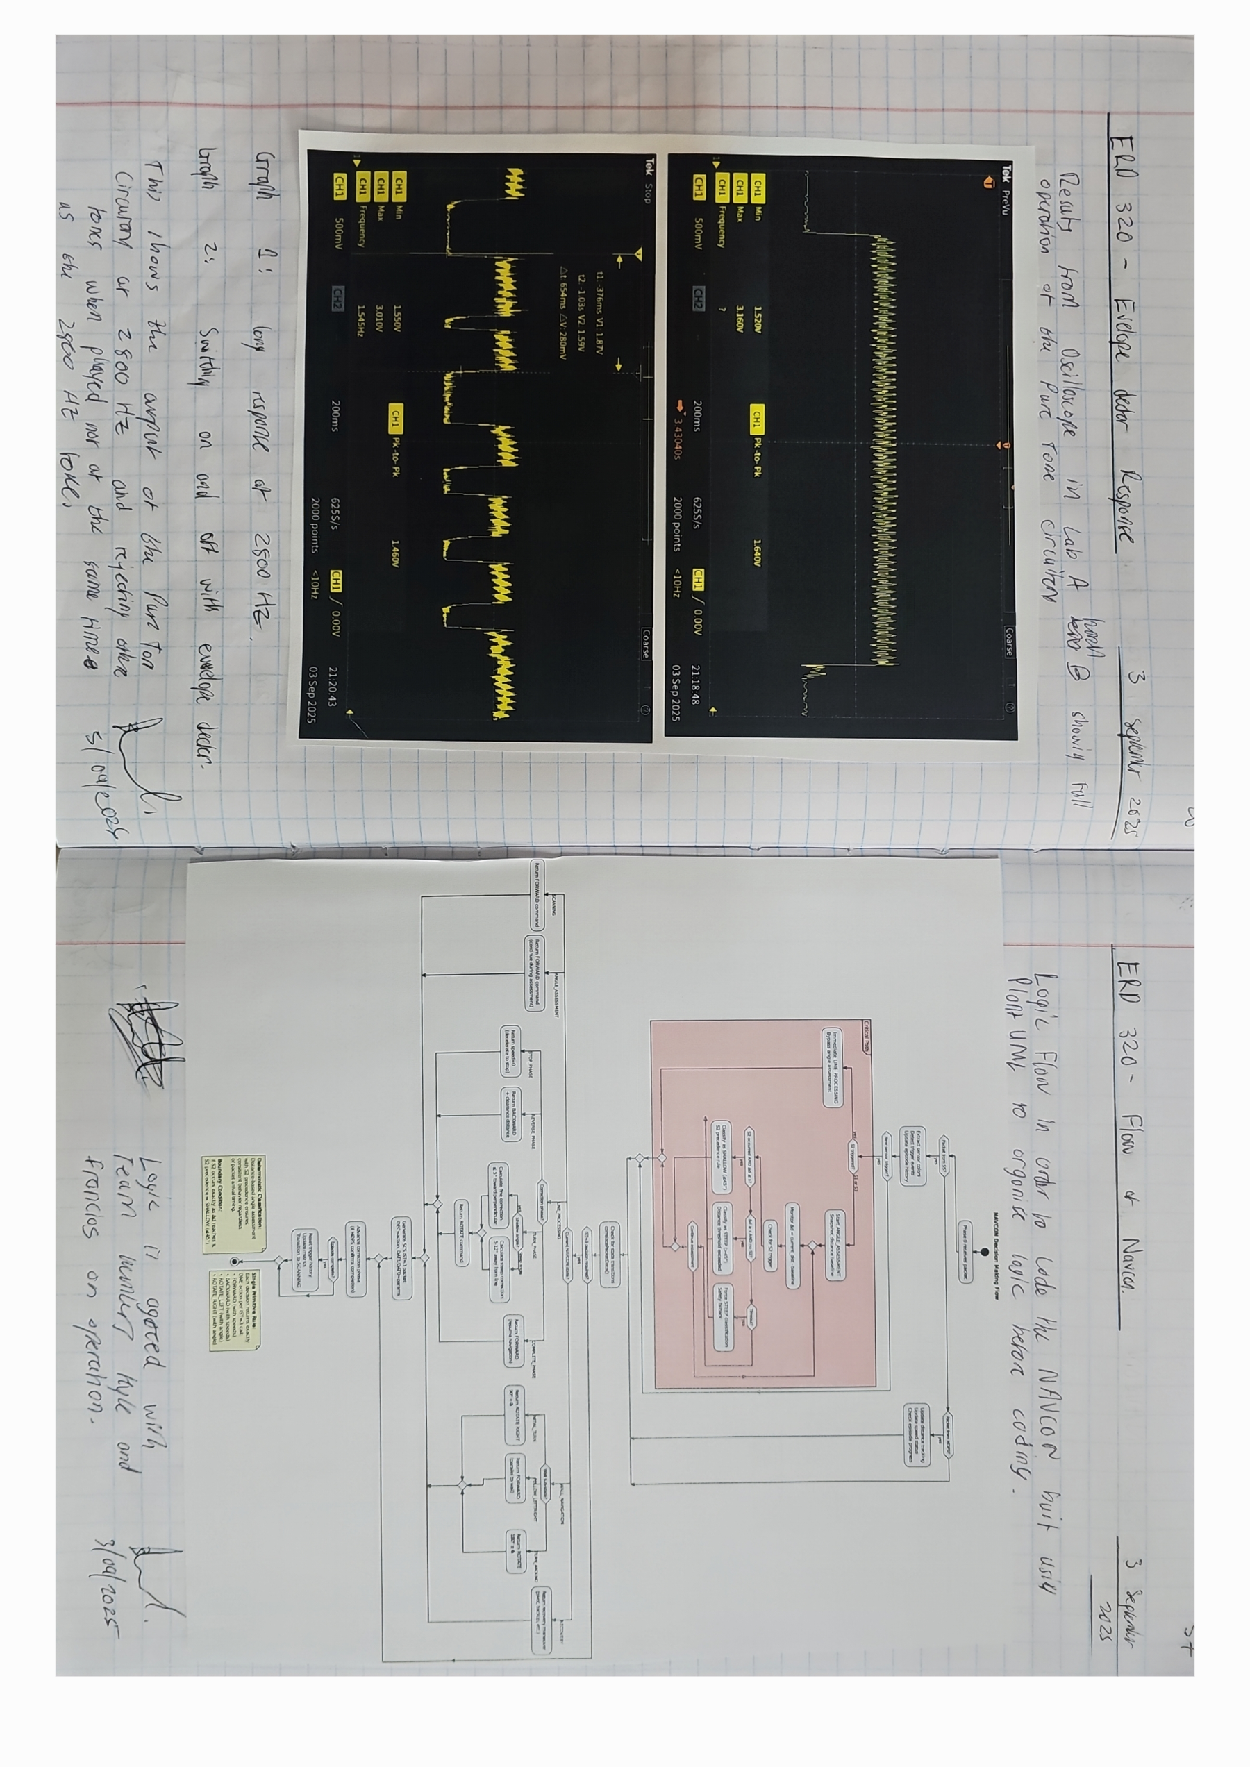
\includegraphics[width=0.9\textwidth]{01_SNC/Labbook/labbook_coding.pdf}
\caption{Lab book excerpt: Approach to firmware coding and testing}
\label{fig:labbook-coding-testing}
\end{figure}



\newpage

% ============================================================================
% SUBSYSTEM 3
% ============================================================================
\section{Subsystem 3: MDPS}
%\textit{Maximum 20 pages per subsystem (excluding lab book excerpts).}

%\subsection{Title: Subsystem 3: MDPS}

\textbf{Subsystem Name:} Motor Driver and Power Supply (MDPS) Subsystem

\textbf{Student Name:} Kyle Green

\textbf{Student Number:} 21441325
\subsection{Subsystem Needs Analysis}

\noindent
The design and construction of a Microcontroller-based Autonomous Robotic Vehicle (MARV) capable of navigating through a maze using predetermined navigation rules requires the development of multiple interacting subsystems. These subsystems must communicate effectively to function as a cohesive unit and achieve the overall task. In particular, a Sensor Subsystem (SS) is required to detect and measure the MARV’s surrounding environment, a State-and-Navigation Control (SNC) subsystem is needed to interpret sensor data and execute decision-making protocols, and a Motor Driver and Power Supply (MDPS) subsystem must supply power to all components and control the MARV’s movement. Together, these three subsystems fulfil the essential functions of detection, processing, and actuation.\\

\noindent
Focusing on the MDPS subsystem, there is a need to control the MARV’s speed and direction based on commands received from the State-and-Navigation Control (SNC) subsystem, and it must measure the MARV’s speed, distance travelled, and rotational displacement. The MDPS must also supply power to all subsystems to enable operation independent of external power sources. In addition, the MDPS must be able to receive and transmit information to and from the SNC and SS.


\subsection{Subsystem Concept Exploration}
% \textit{-	Refer to Kossiakoff, Chapter 6, 7 and 8\\
% -	Do a brief survey of literature on possible methods / circuits / designs that could meet the above needs, other than the prescribed subsystem. MAKE SURE THAT THE DOCUMENTS YOU REFERENCE ARE INCLUDED IN SECTION 1.2!!!}

\noindent
Various approaches can be considered to address the needs of the Motor Driver and Power Supply (MDPS) subsystem. By reviewing multiple sources and evaluating the advantages and disadvantages of each option, a more informed decision can be made regarding the concept best suited for the intended application.

\subsubsection{Movement}
Standard wheels, continuous tracks, cams, or propellers are some of the many options that can be considered when exploring different modes of movement for the MARV.

\begin{table}[H]
\centering
\caption{Comparison of Different Motion Systems}
\label{tab:motion_systems}
\begin{tabular}{|c|p{6cm}|p{6cm}|}
\hline
\textbf{System} & \textbf{Advantages} & \textbf{Disadvantages} \\ \hline
Wheels & Simple Design, Low Cost, Manoeuvrability & Dependence on Flat Surfaces \\ \hline
Tracks & Improved Traction, Better Weight Distribution & Complex Design, Lower Speed \\ \hline
Cams & Simple Design, Precision Motion & Friction Losses, High Torque Required \\ \hline
Propellers & Independence of Ground Terrain  & Complex Design, Manoeuvrability \\ \hline
\end{tabular}
\end{table}

Table \ref{tab:motion_systems} shows that wheeled systems offer a simple design, low production cost, and good manoeuvrability, but they perform best on flat surfaces and may struggle on rough or uneven terrain. Tracked systems provide improved traction and better weight distribution, making them suitable for uneven and smooth surfaces \cite{AUTODESK}, but they are mechanically more complex and generally slower. Cam-based mechanisms is just a lever arm which spins off-centre from the shaft, which can achieve precise motion and maintain a simple design \cite{AUTODESK}, but they suffer from friction losses and require high torque if lifting a system of of the ground. Propeller-based systems allow the vehicle to move independently of ground terrain, which is advantageous for unconventional surfaces \cite{JOUAV}, but they introduce higher complexity and manoeuvrability is significantly reduce when confined to small areas such as the maize. Considering the MARV’s operational environment being a maze with reasonably flat surfaces and the desire for low-cost, with easily controllable motion, a wheeled system is the most appropriate choice. It provides the necessary balance of simplicity and precision that is required to accurately navigate the maze.

\subsubsection{Power}
A simple voltage regulator or dc-dc (buck-boost) converter can be considered to regulate the power of the system. 

\begin{table}[H]
\centering
\caption{Comparison of Power Systems}
\label{tab:power_systems}
\begin{tabular}{|c|p{6cm}|p{6cm}|}
\hline
\textbf{System} & \textbf{Advantages} & \textbf{Disadvantages} \\ \hline
Voltage Regulator & Simple Design, Low Cost, Few Components & Large Losses, Only Step-Down Operations Possible \\ \hline
Buck Converter & Wide Input Voltage, Stable Outputs, Smaller Losses & Cost, More Complex \\ \hline
\end{tabular}
\end{table}

From Table \ref{tab:power_systems}, voltage regulators offer a simple design with low cost and require relatively few components, making them easy to integrate. However, they are limited to step-down operation and can exhibit larger power losses compared to switching converters \cite{VREG}. Buck converters, provide stable outputs over a wide input voltage range and are generally more efficient, but they are more complex and costly, requiring additional components and careful design considerations \cite{DCDC}. Considering  simplicity, low cost, and ease of integration as the driving factors, the voltage regulator is the most suitable choice for the power subsystem, as it meets the operational needs of supplying stable voltage to the subsystems without introducing unnecessary complexity.

\subsubsection{Communication}
\noindent
$I^2C$, SPI, and UART are widely used communication protocols in embedded systems due to their simplicity and reliability, and were therefore considered as potential options for the MARV subsystem.

\begin{table}[H]
\centering
\caption{Comparison of Communication Protocols}
\label{tab:com_systems}
\begin{tabular}{|c|p{6cm}|p{6cm}|}
\hline
\textbf{Protocol} & \textbf{Advantages} & \textbf{Disadvantages} \\ \hline
$I^2C$ & Simple two-wire interface, Multiple slaves and multi-master, error checking & Requires addressing, Half-duplex \\ \hline
SPI & Full-duplex, Single-master systems & Separate slave select lines for each device, Complex wiring for multiple slaves, Limited multi-master support \\ \hline
UART & Simple two-wire interface, bidirectional, asynchronous, configurable baud rate, widely supported for device-to-device communication & Requires matching baud rates between devices \\ \hline
\end{tabular}
\end{table}

From Table \ref{tab:com_systems}, $I^2C$ provides a simple two-wire interface and supports multiple slave devices with built-in error checking, but complexity increases with addressing. SPI offers full-duplex capability, making it ideal for high-speed data transfers, but adding multiple devices increases wiring complexity and it does not easily support multi-master configurations. UART is a simple, asynchronous two-wire protocol that supports bidirectional communication, making it a reliable device-to-device communication protocol \cite{Coms}. Given the MARV’s requirement for asynchronous communication between microcontroller subsystems, and the limited number of devices involved, UART is the most appropriate choice, due to its ease of implementation to meet the operational needs of the system.

% 
\subsection{Subsystem Concept Definition: Planning}
% \textit{-	Refer to Kossiakoff, Chapter 9\\
% -	Provide a single-figure subsystem functional diagram\\
% \hspace*{2em}o	Extend on the practical guide diagram with more details, unique to your design.\\
% \hspace*{2em}o	Include direction and nature of all internal and external interactions, including those with other subsystems and those with the outside world.\\
% -	Provide a single-figure subsystem architecture diagram\\
% \hspace*{2em}o	Extend on the practical guide diagram with more details, unique to your design.\\
% \hspace*{2em}o	Draw to component / software function level \\
% \hspace*{2em}o	Include direction and nature of all internal and external interactions, both to the external world and to other subsystems \\
% \hspace*{2em}o	Indicate clearly which components are designed and which components are bought off-the-shelf. \\
% \textbf{-	This must be more detailed than the diagrams in the practical guide; copies of the practical guide figures will receive 0 marks. }}

% Add your concept definition and diagrams here

\noindent
The Motor Driver and Power Supply (MDPS) subsystem provides both the mechanical actuation and electrical power required for the MARV to operate. Functionally, the MDPS accepts motion commands from the SNC and converts them into controlled wheel movement using its motor actuation hardware. Through this, the subsystem enables the MARV to accelerate, decelerate and perform rotational movements required to navigate the maze. In addition to motion control, the MDPS is responsible for supplying suitable regulated voltage to all connected subsystems. This ensures that the system will operate reliably under varying load conditions. The chosen power approach uses a simple active voltage regulation strategy, which aligns with the MARV’s requirement for stable, low-noise supply rails without unnecessary circuit complexity. The MDPS also incorporates on-board measurement capabilities to support system-level navigation. Using wheel-mounted rotary encoders, the subsystem determines the distance travelled and the angular rotation achieved during turns. These measurements are transmitted to the SNC via asynchronous UART communication.\\

Conceptually, the MDPS therefore acts as both the “movement unit” and the “power distribution unit” of the MARV. It executes movement on request, regulates the system’s electrical supply, and provides movement data to the SNC. Within the broader system architecture, the MDPS serves as the interface between the SNC’s navigation decisions and the MARV’s physical behaviour in the maze environment.

The overall operation of the MDPS subsystem can be seen with the functional block diagram shown in Figure \ref{fig:MDPS_Func} below. 

\begin{figure}[H]
    \centering
    \includegraphics[width=1\textwidth]{03_MDPS/documents/Functional_Block_Diagram.png}
    \caption{MDPS Functional Block Diagram}
    \label{fig:MDPS_Func}
\end{figure}

The overall architecture of the MDPS subsystem can be seen with the architectural diagram shown in Figure \ref{fig:MDPS_Arc} below. 
\subsection{Subsystem Engineering Design}
\textit{- Refer to Kossiakoff, Chapter 13, 15 and 16\\
-	In Section 2.8, attach a one-page excerpt from your handwritten lab book as an example for each heading in this section (eight pages in total)}

\subsubsection{Constraints and trade-offs}

\subsubsubsection{Design Constraints}
\textit{-	Where were you constrained in implementation of the concept?}

% Write about design constraints here

\subsubsubsection{Trade-offs}
\textit{-	Which trade-offs did you consider? How did you make your eventual selections, and why?}

% Write about trade-offs here

\subsubsection{Tools and Methods}

\subsubsubsection{Engineering tools}
\textit{-	Discuss the engineering tools that you used (hardware tools, simulation packages, etc) and motivate their use. This does NOT mean physical hand tools like soldering irons, pliers, etc!}

% Write about engineering tools here

\subsubsubsection{Engineering methods}
\textit{-	Discuss the engineering methods that you used (design methods, prototyping approach, simulation, test benches, etc) and motivate their use. Did you apply agile, waterfall, V-shaped development? If you used parameter sweeps and CAD-based design methods, describe them here. }

% Write about engineering methods here

\subsubsection{Selected design details}
\textit{-	Provide selected details of your design, including circuit schematics, simulation results. Start out by listing which design elements (circuits, code snippets) you will present.}

\subsubsubsection{Statements of requirements}
\textit{Briefly state the high-level requirements of your individually designed circuits and / or code segments.}

% Write your requirements here

\subsubsubsection{Development}
\textit{-	Demonstrate top-down definition with bottom-up implementation (or some other approach commensurate with your selected design approach) of your selected detail designs, motivated by flow charts, design equations, or some other guiding input. }

% Write about development here

\subsubsubsection{Simulations}
\textit{-	Where appropriate, demonstrate circuit simulations, test bench operation, or some other form of computer verification of operation prior to deployment.}

% Add simulations here

\subsubsubsection{Approach to coding and testing}
\textit{-	Describe your approach to microcontroller coding and code testing, with selected examples.}

% Write about coding and testing here

\input{03_MDPS/5_qualification_tests.tex}
\subsection{Subsystem Conclusions and Recommendations}
\textit{-	Does the subsystem adhere to the requirements set out? If not, why not?\\
-	What are the benefits and shortcomings of the subsystem?\\
-	What future work do you recommend for the subsystem?}

% Write your conclusions and recommendations here

\subsection{Lab Book Excerpts}
\stepcounter{subsubsection}  % Increment the section number manually
\subsubsection*{\thesubsubsection\hspace{1em} Design Constraints}
% Add lab book excerpt for design constraints

\stepcounter{subsubsection}  % Increment the section number manually
\subsubsection*{\thesubsubsection\hspace{1em} Trade-offs}
% Add lab book excerpt for trade-offs

\stepcounter{subsubsection}  % Increment the section number manually
\subsubsection*{\thesubsubsection\hspace{1em} Engineering tools}
% Add lab book excerpt for engineering tools

\stepcounter{subsubsection}  % Increment the section number manually
\subsubsection*{\thesubsubsection\hspace{1em} Engineering methods}
% Add lab book excerpt for engineering methods

\stepcounter{subsubsection}  % Increment the section number manually
\subsubsection*{\thesubsubsection\hspace{1em} Statements of requirements}
% Add lab book excerpt for statements of requirements

\stepcounter{subsubsection}  % Increment the section number manually
\subsubsection*{\thesubsubsection\hspace{1em} Development}
% Add lab book excerpt for development

\stepcounter{subsubsection}  % Increment the section number manually
\subsubsection*{\thesubsubsection\hspace{1em} Simulations}
% Add lab book excerpt for simulations

\stepcounter{subsubsection}  % Increment the section number manually
\subsubsection*{\thesubsubsection\hspace{1em} Approach to coding and testing}
% Add lab book excerpt for approach to coding and testing



\end{document}
